\documentclass[12pt,a4paper]{article}
\usepackage[utf8]{inputenc}
\usepackage[american]{babel}
\usepackage{ragged2e}
\usepackage{amsmath, amsfonts, amsthm, amssymb, graphicx, lipsum}
\usepackage[]{acronym}
\usepackage{hyperref}
\usepackage{times}
\usepackage[export]{adjustbox}
\usepackage[inkscapearea=page]{svg}
\usepackage{tabularx}
\usepackage{booktabs}
\usepackage{mathtools,bm}
\usepackage{mathrsfs}
\usepackage{float}
\usepackage{enumitem}
\usepackage{mathtools}
\usepackage{fancyhdr}
\usepackage{geometry}
\usepackage{svg}
\usepackage{tabularx}
\usepackage{titlesec}
\usepackage{fancyvrb}
\usepackage{fancyhdr, lastpage}
\usepackage{csquotes}
\usepackage[backend=biber, sorting=none, sortcites=true, style=ieee]{biblatex}
\usepackage{caption}
\usepackage{subcaption}
\usepackage{listings}
\usepackage{xcolor}
\usepackage{pifont}
\newcommand{\cmark}{\ding{51}}%
\newcommand{\xmark}{\ding{55}}%

% TikZ for diagrams
\usepackage{tikz}
\usetikzlibrary{positioning,fit,arrows.meta,backgrounds,shapes.geometric,calc,shadows,decorations.pathreplacing}


\definecolor{codegray}{rgb}{0.5,0.5,0.5}
\definecolor{backcolour}{rgb}{0.95,0.95,0.92}

\lstdefinestyle{mystyle}{
    backgroundcolor = \color{backcolour},
    captionpos= b,
    showspaces= false,
    breakatwhitespace = false,
    basicstyle=\small,
    showtabs=false,
    tabsize = 1,
    numbersep=5pt,
    xleftmargin=0.7cm,
    frame=tlbr,
    framesep=0.2cm, 
    framerule=0pt,
}

\lstset{style=mystyle}

\DeclareLanguageMapping{american}{american-apa}

\addbibresource{src/ref.bib}

\hypersetup{
    colorlinks=true,
    linkcolor=black,
    urlcolor=black,
    citecolor=black,
    pdftitle={Graduation project},
}
\geometry{
 a4paper,
 margin=40mm,
 right=20mm,
 bottom=30mm,
 }
\renewcommand{\baselinestretch}{1.5}

 
\renewcommand{\labelitemii}{$\circ$}

\pagenumbering{roman}

\begin{document}

\begin{titlepage}
    \begin{center}
    
        \large

         \textbf{FRAMEWORK FOR TRAINING AND DEPLOYMENT OF LOCOMOTION FOR HUMANOID ROBOTS BASED ON DIGITAL TWINS AND REINFORCEMENT LEARNING}
        
        \bigskip
        
        \large
            
        by
        
        \bigskip
        
        \bigskip
        
        Juan Andrés Méndez G.
        
        \bigskip
        
        Submitted to the
        
        \smallskip
        
        Department of System \& Computing Engineering
        
        \smallskip
        
        in Partial Fulfillment of the Requirements for the Degree of 
        
        \bigskip
        
        Masters in Systems \& Computing Engineering
        
        \bigskip
        
        at the 
        
        \bigskip
        
        University of the Andes 
        
        \bigskip
        
        Jan 2026
        
        \vspace{2cm}
        
        © 2026 University of the Andes. All rights reserved.
        
        \normalsize
        \medskip
        
        \begin{center}
        Thesis Supervisors
        \end{center}
        
        \begin{tabular}{@{}p{4.5cm}@{\hspace{0.5cm}}p{4.5cm}@{\hspace{0.5cm}}p{4.5cm}@{}}
            Carlos Andrés Lozano Garzón \\
            Ph.D. in Technology \\
        \end{tabular}
    
            

    \end{center}
\end{titlepage}



\newpage


\vspace*{10px}

\begin{center}


\Large

 \textbf{FRAMEWORK FOR TRAINING AND DEPLOYMENT OF LOCOMOTION FOR HUMANOID ROBOTS BASED ON DIGITAL TWINS AND REINFORCEMENT LEARNING}
\vspace{1cm}

\large

by

\medskip

Juan Andrés Méndez G.


\bigskip

Submitted to the


Department of Systems \& Computing Engineering


on \today \: in Partial fulfillment of the 


Requirements for the Degree of 

\bigskip

Masters in Systems \& Computing Engineering

\end{center}

\normalsize

\vspace{1cm}

\addcontentsline{toc}{section}{Abstract}

\section*{Abstract:}

Humanoid robot locomotion continues to pose fundamental challenges in reinforcement learning deployment, particularly regarding the simulation-to-reality transfer gap, hardware safety during experimental training, and control complexity in high-degree-of-freedom articulated systems. Despite recent advances in deep reinforcement learning and physics simulation, the transition from simulated policies to physical robots remains a critical bottleneck in robotics research and education, where limited hardware access and damage risks significantly constrain iterative development. This thesis investigates the hypothesis that end-to-end reinforcement learning can achieve effective goal-directed navigation for high-DOF humanoid robots without hierarchical decomposition into trajectory planning and gait generation, and that simulation-to-simulation transfer using authentic communication protocols serves as a viable intermediate validation step. The research develops and validates a comprehensive framework for the Unitree G1 humanoid robot using NVIDIA Isaac Lab, implementing a custom reinforcement learning task for goal-directed point-to-point navigation using Proximal Policy Optimization (PPO) operating on proprioceptive observations across 29 actuated degrees of freedom. The framework achieves 87\% goal success rate with stable bipedal locomotion, supporting the central hypothesis. A simulation-to-simulation (sim2sim) verification framework employing authentic ROS 2 Humble protocols enables policy evaluation under communication realistic conditions prior to physical deployment. Exploratory work on social navigation infrastructure---integrating LiDAR-based obstacle perception with proximity-aware reward shaping---revealed fundamental reward design challenges: the policy achieved only 1\% goal success rate, demonstrating that multi-objective reward formulations for simultaneous goal-seeking and obstacle avoidance require substantial redesign, with documented analysis identifying specific gradient imbalances that inform future approaches. While systematic latency characterization and effective social navigation remain as future work, the established infrastructure provides a validated foundation for safer sim-to-real transfer in educational and research contexts where physical robot access is limited.


\medskip

\phantomsection

\addcontentsline{toc}{subsection}{Keywords}

\subsection*{Keywords:}
Digital Twins, Humanoid Robots, Deep Reinforcement Learning, Sim-to-Sim Validation, ROS 2, NVIDIA Isaac Lab, Unitree G1, Locomotion Control, PPO Algorithm, Social Navigation, LiDAR Perception



\newpage

\medskip

\addcontentsline{toc}{section}{Acknowledgements}
\section*{Acknowledgements}

The completion of this thesis would not have been possible without the guidance, support, and encouragement of remarkable individuals who have shaped both my academic journey and personal growth.


I extend my deepest gratitude to my thesis supervisor and dear friend, \textbf{Dr. Carlos Andrés Lozano Garzón}. His exceptional depth of knowledge in IoT, Cybersecurity, and Metaheuristics Optimization provided the intellectual foundation for this work. Yet beyond his technical expertise, it was his profoundly humane treatment, unwavering comprehension, and patient guidance that made this journey possible. His mentorship extended far beyond what any thesis supervisor is expected to provide, and for that, I am forever grateful.

I am deeply thankful to \textbf{Dr. Germán Adolfo Montoya Orozco}, whose teaching in my first optimization course ignited a passion that ultimately guided me toward this Master's degree and my enduring interest in robotics. His ability to inspire curiosity in complex subjects left a lasting impression on my academic path.

My sincere appreciation goes to \textbf{Dr. Edgar Alejandro Marañón León}. His companionship throughout this process and his contagious enthusiasm for the applications of artificial intelligence in mechanical engineering enriched my perspective and motivated me to explore interdisciplinary approaches.

I am profoundly grateful to \textbf{Dr. Alejandra Tabares Pozos}, Assistant Professor in the Department of Industrial Engineering. Her trust and belief in my capabilities opened doors that fundamentally shaped this research. The opportunity to work closely with the Ambiente Integrado de Aprendizaje (AIA) laboratory, which she is part of, provided the essential infrastructure and collaborative environment that made this thesis possible.

Special thanks to \textbf{Álvaro Urel Achury}, laboratory assistant at the Colibri robotics facility, for his patience and willingness to share his deep knowledge of the Unitree G1 humanoid robot. His practical expertise and generous support were invaluable in bridging the gap between theoretical concepts and hands-on implementation.


To my \textbf{mother}: words cannot adequately express the depth of my gratitude for the extraordinary care and love you provided throughout the countless long nights and demanding days---not only during this Master's program but throughout my entire undergraduate journey as well. Your unwavering support, quiet sacrifices, and endless encouragement have been an incalculable source of strength. This achievement is as much yours as it is mine.

To my \textbf{father}: you are my inspiration for pursuing studies in STEM. You taught me, through your example and words, that anything is possible with sufficient effort and dedication. Beyond being the first engineer I ever knew, you have always been a great human being whose integrity and work ethic continue to guide my path. Thank you for showing me what excellence truly means.

\vspace{0.5cm}
\noindent To all of you---mentors, colleagues, friends, and family---this work stands as a testament to your collective influence on my life. Thank you.


\phantomsection

\newpage

\addcontentsline{toc}{section}{Contents}

\phantomsection

\tableofcontents

\newpage

\addcontentsline{toc}{section}{List of tables}

\phantomsection

\listoftables

\newpage

\addcontentsline{toc}{section}{List of figures}

\phantomsection

\listoffigures

\newpage

\addcontentsline{toc}{section}{Acronyms}
\section*{Acronyms}

\begin{acronym} [PCNA]
   \acro{rl}   [RL]    {Reinforcement Learning}
   \acro{drl}  [DRL]   {Deep Reinforcement Learning}
   \acro{ros}  [ROS]   {Robot Operating System}
   \acro{dof}  [DOF]   {Degrees of Freedom}
   \acro{gpu}  [GPU]   {Graphics Processing Unit}
   \acro{ppo}  [PPO]   {Proximal Policy Optimization}
   \acro{urdf} [URDF]  {Unified Robot Description Format}
   \acro{usd}  [USD]   {Universal Scene Description}
\end{acronym}

\newpage

\pagenumbering{arabic}

\section{Introduction}

The field of humanoid robotics is undergoing significant transformation in 2023-2026, characterized by substantial cost reductions, advanced integration of artificial intelligence integration, and expanding educational applications. The humanoid robotics market, projected to reach \$38 billion by 2035, is experiencing rapid changes driven by platforms that reduce costs by up to 90\% compared to previous generations \parencite{marketsandmarkets2024}. This shift is reshaping how educational and research institutions approach robotics, creating opportunities for universities to engage with advanced technology that was previously financially inaccessible.

Humanoid robots represent one of the most complex and promising domains in contemporary engineering, designed to navigate and interact within environments originally conceived for humans. These platforms face substantial challenges in design, control, and programming derived from their elevated kinematic and dynamic complexity \parencite{radosavovic2024realworld}. The development of robust behaviors has historically been constrained by prohibitive hardware costs, system vulnerability during experimental training, and the difficulty of controlling devices with dozens of degrees of freedom \parencite{gu2024humanoidgym}. These limitations have created significant barriers for educational institutions seeking to incorporate advanced robotics into their curricula and research programs.

The Laboratorio Colivri (Collaboration Laboratory for Interaction, Visualization, Robotics and Autonomous Systems) at the Universidad de los Andes exemplifies these challenges on a scale. Since 2025, the laboratory has had single Unitree G1 humanoid robot to serve the educational and research needs of more than 8,000 engineering students. This situation creates three critical operational challenges that demand innovative solutions:

First, the \textbf{scalability and logistics} challenge emerges from having only one robot available for an entire academic community. Programming practices, projects, and demonstrations are severely limited, with no efficient mechanism to guarantee equitable usage time between courses and research groups. The planned exhibition activities—where the G1 must navigate the laboratory and demonstrate capabilities to visitors—compete directly with teaching schedules and development time, creating severe operational bottlenecks that limit the robot's educational impact.

Second, the \textbf{safety and preservation of hardware} are in paramount,  given that the G1 represents a substantial investment for the laboratory. The robot, with its approximately 35 degrees of freedom and complex contact dynamics, faces inherent risks when new locomotion routines are tested directly on the physical hardware \parencite{unitree2024}. Damage from falls, overcurrents, or control instabilities would result in elevated repair costs and extended downtime periods, potentially disrupting entire academic semesters.

Third, the \textbf{advanced functional requirements} imposed as purchase conditions demand sophisticated capabilities. The robot must perform exhibition tasks including navigating autonomously through the laboratory and demonstrating various locomotion behaviors. These requirements necessitate robust navigation policies capable of goal-directed movement and dynamic balance—capabilities that traditionally require extensive training and validation cycles.

Recent technological advances offer a promising framework to address these challenges. The emergence of high-fidelity physical simulation platforms, such as NVIDIA Omniverse Isaac Sim, enables the creation of digital twins capable of accurately reproduce contact dynamics, friction, and material deformation with high precision \parencite{nvidia2024isaac}. Deep reinforcement learning techniques have demonstrated remarkable effectiveness in synthesizing control policies for systems with multiple degrees of freedom, particularly when employing hierarchical approaches, progressive curricula, or model-based methods \parencite{humanoidgym2024}. Furthermore, the integration of standardized robotics middleware like ROS 2 provides reliable communication protocols that can bridge simulation and physical deployment environments.

The convergence of these technologies—accessible hardware platforms, advanced simulation environments, and proven reinforcement learning methods—creates a significant opportunity to increase accessibility of advanced robotics education. Unitree G1, at approximately \$16,000 for basic configurations, represents a 90\% cost reduction over previous-generation humanoids, making it accessible to institutions previously priced out of humanoid robotics research. With 23-43 degrees of freedom depending on configuration, integrated NVIDIA Jetson Orin processing delivering 100 TOPS of AI capability, and comprehensive sensor suites including depth cameras and 3D LiDAR, the G1 provides a capable platform for exploring advanced locomotion control.

This thesis proposes the development of an integrated methodological framework that combines two core technological components—digital twins and deep reinforcement learning to safely and efficiently train and validate locomotion policies for the Unitree G1. The framework addresses the fundamental barriers that have limited progress in humanoid robotics while providing a scalable solution for educational institutions facing similar challenges. Through the construction of a high-fidelity digital twin of both the robot and its operational environment, the methodology enables extensive experimentation without physical risks. By applying deep reinforcement learning with Proximal Policy Optimization, the system facilitates the synthesis of robust locomotion and navigation policies. Critically, by implementing a simulation-to-simulation validation environment that uses authentic ROS 2 communication protocols, the framework provides a credible intermediate step before costly physical deployment, substantially mitigating the simulation-to-reality transfer gap.

The central hypothesis of this research is that end-to-end reinforcement learning can achieve effective goal-directed navigation for high-DOF humanoid robots without requiring hierarchical decomposition into separate trajectory planning and gait generation modules, and that simulation-to-simulation transfer using authentic communication protocols can serve as a viable intermediate validation step before physical deployment. This hypothesis challenges the conventional approach to humanoid locomotion, which that typically decomposes the problem into distinct layers—high-level path planning, mid-level trajectory generation, and low-level gait control—by demonstrating that a single learned policy operating directly on joint-level actions can produce stable, goal-directed locomotion. Additionally, the research explores whether LiDAR-based obstacle perception can be integrated into such policies for social navigation, documents the design challenges that emerge from multi-objective reward formulations and informs future approaches to human-aware humanoid locomotion.

The proposed methodology seeks to achieve multiple interconnected objectives: significantly reducing hardware damage risk and associated costs; accelerating iteration cycles through exhaustive simulation validation; validating learned policies under realistic communication constraints; and enabling broader robot access among the thousands of students who use the Laboratorio Colivrí. While the study focuses on the Unitree G1 within a specific institutional context, the approach is deliberately generalizable, intended to lay the foundations for other institutions to adopt similar solutions with different humanoid platforms and varied operational contexts. This research thus offers a scalable contribution to the fields of humanoid robotics and systems engineering, addressing the fundamental barriers that have limited the progress of these highly articulated systems in educational settings.


\section{Objectives}

\subsection{General Objective}

Develop a framework for training and validating locomotion policies for the G1 humanoid robot using digital twins and deep reinforcement learning, achieving goal-directed navigation capabilities while enabling safe policy development in simulation and validation through simulation-to-simulation transfer using ROS with a preliminary exploration of social navigation infrastructure to establish foundations for future research.

\subsection{Specific Objectives}
\begin{itemize}
    \item Create a high-fidelity digital twin of the Unitree G1 humanoid robot in NVIDIA Isaac Lab, accurately incorporating its physical, kinematic, and sensorial properties to enable safe and scalable experimentation.

    \item Design and implement a deep reinforcement learning task using Proximal Policy Optimization (PPO) for goal-directed point-to-point navigation through low-level joint control across 29 DOF, achieving stable bipedal locomotion with high goal success rates.

    \item Develop a simulation-to-simulation (sim2sim) validation framework that employs authentic ROS 2 Humble communication protocols, enabling policy evaluation under realistic message passing patterns and asynchronous communication constraints before physical deployment.

    \item Explore infrastructure for human-aware locomotion as preliminary groundwork for future research, implementing LiDAR sensor integration, dynamic obstacle simulation representing pedestrians, and graduated proximity penalty functions, while documenting the technical challenges encountered that inform subsequent reward design improvements.

    \item Validate the trained locomotion policies in the sim2sim environment, evaluating performance metrics including locomotion stability, goal-reaching accuracy, and policy robustness under ROS 2 transport layer constraints.
\end{itemize}

\newpage

\section{Literature Review}

The development of autonomous humanoid robots capable of adaptive locomotion requires integrating multiple technological domains: robotic platforms, digital twin methodologies, reinforcement learning algorithms, simulation-to-reality transfer techniques, and communication middleware. This literature review examines recent advances in each domain, identifies critical gaps, and positions this thesis within the current research landscape.

\subsection{Humanoid Robot Platforms and Market Evolution}

The humanoid robotics market has experienced substantial growth, driven by technological advances and cost reductions that have increased access to sophisticated platforms. Market analysts project substantial expansion, with Goldman Sachs forecasting the global humanoid robot market could reach \$38 billion by 2035 \parencite{goldmansachs2024humanoid}, while MarketsandMarkets estimates growth from \$1.8 billion in 2023 to \$13.8 billion by 2028 at a compound annual growth rate of 50.3\% \parencite{marketsandmarkets2024}.

This rapid market expansion reflects a fundamental shift from expensive research platforms to commercially viable products. Contemporary humanoid platforms demonstrate increasing accessibility: Boston Dynamics' Atlas Electric showcases advanced hydraulic-free actuation; Figure AI's Figure 02 integrates vision-language models for manipulation tasks; Tesla's Optimus Gen 2 emphasizes manufacturing scalability; 1X Technologies' NEO targets consumer applications; and Apptronik's Apollo focuses on logistics and warehouse automation. Notably, the cost of capable humanoid platforms has decreased approximately 90\% over the past decade, with current educational-grade platforms available at price points accessible to universities and research institutions.

The Unitree G1 humanoid robot, central to this thesis, exemplifies trend toward accessibility . With 29 degrees of freedom distributed across hip (3-DOF), knee (1-DOF), ankle (2-DOF), waist (3-DOF), shoulder (3-DOF), elbow (1-DOF), and wrist (1-DOF) joints, the G1 provides sufficient kinematic complexity for research-grade locomotion and manipulation tasks \parencite{unitree2024}. The platform integrates an NVIDIA Jetson Orin onboard computer, enabling local neural network inference, and incorporates multiple sensor modalities, including 3D LiDAR, stereo depth cameras, and a 6-axis inertial measurement unit. This combination of affordability, computational capability, and sensor integration makes the G1 particularly suitable for educational contexts where hardware budgets are constrained, but research requirements remain demanding.

The proliferation of affordable humanoid robots creates an urgent demand for safe, scalable training methodologies suitable for educational contexts where hardware access is severely limited. A single physical robot must often serve hundreds or thousands of students, making destructive training approaches—such as direct trial-and-error learning on hardware—economically and pedagogically infeasible. This constraint motivates the development of intermediate validation frameworks that reduce hardware damage risks while maintaining research-grade capabilities.

\subsection{Digital Twins for Robotics}

Digital twins represent virtual replicas of physical systems that enable safe experimentation, analysis, and validation without the risks and costs associated with physical prototypes. \textcite{hasan2023decoding} define digital twins as dynamic virtual models that continuously synchronize with their physical counterparts through bidirectional data exchange, enabling prediction, optimization, and decision-making. This bidirectionality distinguishes digital twins from conventional simulations: while simulations model hypothetical scenarios, digital twins maintain ongoing correspondence with real-world systems.

The creation of accurate digital twins requires systematic physical-to-virtual twinning processes. \textcite{sturm2021creation} identify three critical dimensions: geometric accuracy (capturing physical dimensions and spatial relationships), kinematic fidelity (representing joint configurations and constraints), and dynamic realism (modeling mass properties, friction, and contact behaviors). In robotics, this twinning process typically involves CAD-to-simulation pipelines that convert mechanical designs into physics-compatible representations, sensor modeling that replicates measurement characteristics and noise profiles, and actuator characterization that captures torque limits, response delays, and control bandwidth.

ROS-based digital twin architectures have emerged as a dominant paradigm for robotic systems. \textcite{digitaltwinros2023development} demonstrate digital twin implementations using ROS 2 for mobile robots, emphasizing the middleware's capabilities for distributed communication, quality-of-service guarantees, and real-time data transport. Their approach employs authentic communication protocols in simulation, enabling validation of control algorithms under realistic message-passing patterns, network latencies, and asynchronous communication constraints—factors often neglected in pure physics simulation.

NVIDIA Isaac Sim and Isaac Lab represent state-of-the-art platforms for creating high-fidelity robotic digital twins \parencite{nvidia2024isaac, nvidia2024isaaclab}. Isaac Sim provides GPU-accelerated physics simulation using the PhysX 5 engine, photorealistic rendering via RTX ray tracing, and accurate sensor models including LiDAR, RGB-D cameras, and IMUs. Isaac Lab extends this foundation with a Python-based framework specifically designed for robot learning, offering reinforcement learning environment abstractions compatible with Gymnasium standards, efficient vectorized simulation enabling thousands of parallel environments on a single GPU, and domain randomization utilities for sim-to-real transfer. The platform supports Universal Scene Description (USD) format scenes, enabling complex environments with realistic visual and physical properties.

Digital twins serve multiple purposes in robotics research: algorithm development and testing in risk-free environments, parameter tuning without hardware wear, failure mode analysis under extreme conditions, and scalable training through massively parallel simulation. However, a critical question remains to be addressed in existing digital twin work: how can policies trained in simulation be credibly validated before deployment to physical hardware? Most frameworks assume sufficient domain randomization or direct hardware testing, leaving a credibility gap for educational contexts where hardware damage risks must be minimized. Currently, frameworks integrate digital twins with robust intermediate validation steps before physical deployment, particularly for educational contexts where thousands of students must share limited hardware resources.

\subsection{Reinforcement Learning for Locomotion Control}

Reinforcement learning has emerged as the dominant paradigm for training adaptive locomotion controllers, enabling robots to learn complex behaviors through interaction with the environment. This section examines foundational RL principles before surveying contemporary approaches to humanoid locomotion.

\subsubsection{Foundations of Reinforcement Learning}

Reinforcement learning formalizes the control problem as a Markov Decision Process (MDP) comprising states, actions, transition dynamics, rewards, and a discount factor \parencite{sutton2018reinforcement}. The objective is to learn a policy that maximizes expected cumulative discounted reward. For locomotion control, states typically include joint positions, velocities, angular velocities, and base orientation; actions correspond to joint torque commands or position targets; and rewards encode task objectives such as forward velocity, energy efficiency, and stability.

Policy optimization methods directly learn parametrized policies, with Proximal Policy Optimization (PPO) demonstrating particular effectiveness for robotic control. PPO constrains policy updates to a trust region defined by a clipped objective function, preventing destructively large updates while maintaining sample efficiency. This stability proves critical for physical systems where catastrophic forgetting or unsafe policies could damage hardware. PPO has become the de facto standard for legged robot locomotion due to its balance of sample efficiency, stability, and implementation simplicity.

Simulation-to-reality transfer remains a fundamental challenge in RL-based robotics. Policies trained in simulation often fail when deployed to physical systems due to dynamics mismatch (imperfect modeling of friction, contact, and inertia), sensor noise (simulation sensors providing noiseless measurements), actuator delays (real motors exhibiting bandwidth limitations), and unmodeled effects (cable dynamics, backlash, temperature dependencies). Domain randomization addresses these challenges by training over distributions of simulation parameters—varying masses, friction coefficients, joint damping, sensor noise levels, and control frequencies—encouraging policies to develop robust behaviors that generalize across parameter variations.

\subsubsection{Contemporary Approaches to Humanoid Locomotion}

Recent research demonstrates multiple viable strategies for humanoid locomotion, each with distinct tradeoffs in terms of data requirements, computational demands, infrastructure needs, and deployment accessibility.

\paragraph{Motion Capture and Retargeting Approaches}

\textcite{cheng2024expressive} present a whole-body control framework for humanoid robots that leverages motion capture data to achieve natural, expressive movements. Their approach employs hierarchical control: a high-level policy tracks reference motions from human motion capture datasets, while a low-level controller resolves whole-body dynamics and maintains balance. This architecture enables behaviors such as expressive gestures, dynamic walking with arm swings, and socially appropriate movements suitable for human-robot interaction contexts.

Motion capture-based methods offer significant advantages for applications requiring natural-looking behaviors, such as entertainment robotics, service robots in social settings, and telepresence systems. The learned policies can reproduce complex human movements with high fidelity, providing immediate visual appeal and intuitive motion characteristics. However, these approaches demand substantial infrastructure: motion capture systems with multiple synchronized cameras, human subjects performing relevant behaviors, and motion retargeting pipelines that map human kinematic structures to robot configurations. This infrastructure requirement limits accessibility for educational institutions without dedicated motion capture laboratories.

\paragraph{Transformer-Based In-Context Adaptation}

\textcite{radosavovic2024realworld} demonstrate real-world humanoid locomotion using a causal transformer-based controller capable of in-context adaptation, published in Science Robotics. Their approach trains a large-scale transformer model on diverse simulation experiences, enabling the policy to adapt to novel terrain and disturbances without gradient updates. The controller was deployed to the Digit humanoid robot, achieving zero-shot transfer to outdoor environments and demonstrating adaptation to slopes, uneven terrain, and external pushes.

The key innovation lies in the transformer's ability to leverage sequential context: by processing recent state-action-reward histories, the model infers environmental characteristics and adjusts behavior online. This in-context learning mimics meta-learning, where the model "learns how to learn" during deployment rather than requiring offline retraining. \textcite{radosavovic2024challenging} extend this work to challenging terrain navigation, demonstrating locomotion over obstacles, stairs, and steep inclines.

Transformer-based approaches represent the current state of the art in adaptability and robustness. The models generalize remarkably well to conditions absent from training data, suggesting strong inductive biases learned during large-scale training. However, these capabilities come with substantial computational costs: training requires massive GPU clusters (often hundreds of GPUs for weeks), the models have millions to billions of parameters demanding significant inference computation, and the training data requirements span diverse simulation scenarios necessitating extensive environment engineering. These resource demands place transformer-based methods beyond the reach of most educational institutions, limiting their applicability for student-led research projects.

\paragraph{Direct Reinforcement Learning Approaches}

\textcite{gu2024humanoidgym} present Humanoid-Gym, an open-source reinforcement learning framework specifically designed for humanoid robot locomotion with proven zero-shot sim-to-real transfer capability. Built on NVIDIA Isaac Gym, the framework supports multiple Unitree platforms including H1, G1-29dof, G1-23dof, and B2 robots. The approach employs Proximal Policy Optimization with privileged information during training: the policy has access to ground-truth state information in simulation. However, it relies solely on proprioceptive sensing (joint encoders, IMU) during deployment.

Key methodological components include domain randomization over physical parameters (mass distributions, friction coefficients, joint damping, motor strengths), observation noise injection simulating sensor imperfections, control frequency randomization matching real hardware variability, and careful reward shaping balancing task objectives (forward velocity tracking) with regularization terms (energy efficiency, smooth actions, minimal joint accelerations). The authors demonstrate successful deployment to physical Unitree H1 and G1 robots, validating the framework's sim-to-real transfer capabilities.

Direct RL approaches using PPO offer a compelling balance of accessibility, reproducibility, and proven transfer capability. The training can be conducted on a single workstation with a modern GPU (e.g., NVIDIA RTX 4090 or A100). The algorithms are well-documented with open-source implementations, and the methodology has been validated across multiple physical platforms. This accessibility makes direct RL particularly suitable for resource-constrained educational contexts where students require hands-on experience with state of the art methods but lack access to massive computational infrastructure.

However, existing direct RL frameworks assume zero-shot sim-to-real transfer through domain randomization alone, directly deploying simulation-trained policies to physical hardware after training completion. This approach introduces risk: if domain randomization proves insufficient, the first deployment attempt could damage expensive hardware. For educational contexts where a single robot must serve thousands of students, this risk profile is unacceptable.

\paragraph{Vision-Language-Action Models}

Emerging multimodal approaches integrate vision, language, and action learning for high-level task planning. NVIDIA's GR00T (Generalist Robot 00 Technology) framework enables robots to learn from multimodal demonstrations by combining visual observations with natural-language instructions. \textcite{nature2025llm} present ELLMER, a framework using GPT-4 for adaptive manipulation tasks, demonstrating language-conditioned policy selection and task decomposition.

Vision-language-action models show promise for high-level reasoning and task planning, they currently remain complementary to low-level locomotion control rather than replacing it. Locomotion requires real-time control at high frequencies (50-1000 Hz), demands fast inference latencies incompatible with large language model queries, and benefits from reactive behaviors that bypass deliberative reasoning. This work focuses on low-level locomotion control, acknowledging that future integration with high-level VLA planners represents a promising research direction.

\paragraph{Critical Comparison and Positioning}

The surveyed approaches reveal fundamental tradeoffs between adaptability, accessibility, and deployment risk:

\begin{itemize}
\item \textbf{Transformer-based methods} \parencite{radosavovic2024realworld, radosavovic2024challenging} achieve remarkable adaptability and robustness through in-context learning but require substantial computational resources (hundreds of GPUs, weeks of training) beyond typical educational budgets.

\item \textbf{Motion capture approaches} \parencite{cheng2024expressive} produce natural, expressive behaviors suitable for social robotics but demand specialized motion capture infrastructure unavailable in most educational settings.

\item \textbf{Direct RL methods} \parencite{gu2024humanoidgym} offer accessibility, reproducibility, and proven sim-to-real capability using standard workstation hardware, making them suitable for educational contexts. However, they assume zero-shot transfer through domain randomization alone, introducing hardware damage risks if randomization proves insufficient.
\end{itemize}

Table \ref{tab:rl_comparison} summarizes these tradeoffs quantitatively, highlighting the accessibility advantages of direct RL approaches while identifying the validation gap this thesis addresses.

\begin{table}[H]
\centering
\caption{Comparison of Contemporary Humanoid Locomotion Approaches}
\label{tab:rl_comparison}
\footnotesize
\begin{tabular}{p{2.8cm}|p{3.5cm}|p{3.2cm}|p{3.8cm}}
\hline
\textbf{Dimension} & \textbf{Transformer-Based} \parencite{radosavovic2024realworld} & \textbf{Motion Capture} \parencite{cheng2024expressive} & \textbf{Direct RL} \parencite{gu2024humanoidgym} \\
\hline
\hline
\textbf{Adaptability} & Very High (in-context learning) & Medium (retargeted motions) & Medium-High (learned policies) \\
\hline
\textbf{Infrastructure Required} & 100+ GPU cluster & Motion capture lab & Single GPU workstation \\
\hline
\textbf{Training Time} & Weeks & Days-Weeks & 6-12 hours \\
\hline
\textbf{Inference Cost} & High (millions of parameters) & Medium (hierarchical) & Low (compact network) \\
\hline
\textbf{Educational Accessibility} & Very Low (research labs only) & Low (specialized labs) & High (standard hardware) \\
\hline
\textbf{Validation Strategy} & Direct sim-to-real & Physical testing & Direct sim-to-real with domain randomization \\
\hline
\textbf{Hardware Damage Risk} & Medium & Low (tested motions) & Medium-High \\
\hline
\textbf{Primary Task} & Velocity tracking + terrain adaptation & Expressive whole-body motions & Velocity tracking \\
\hline
\end{tabular}
\end{table}

This thesis adopts the direct RL approach following \textcite{gu2024humanoidgym} for its accessibility and reproducibility, but introduces an intermediate sim-to-sim validation step using authentic ROS 2 communication protocols. This methodological contribution addresses the credibility gap between pure simulation training and costly physical deployment, providing an additional verification layer particularly valuable for educational institutions with limited hardware access. While domain randomization prepares policies for physics variations, authentic communication protocols validate performance under realistic message-passing patterns, latencies, and asynchronous transport characteristics—factors critical for real-world deployment but absent from pure simulation training.

\subsection{Simulation-to-Reality Transfer Methodologies}

Simulation-to-reality (sim-to-real) transfer addresses the challenge of deploying policies trained in simulation to physical robots. Despite advances in simulation fidelity, systematic differences between virtual and real environments—termed the "reality gap"—can cause trained policies to fail during physical deployment.

\subsubsection{Sources of the Reality Gap}

The reality gap arises from multiple sources. Dynamics mismatch occurs when simulation engines imperfectly model friction, contact mechanics, joint flexibility, and inertial properties. Sensor discrepancies arise when simulated sensors provide noiseless, geometrically perfect measurements while real sensors exhibit noise, drift, calibration errors, and sampling artifacts. Actuator differences manifest through unmodeled delays, bandwidth limitations, backlash, and torque ripples. Environmental factors such as air resistance, temperature effects, cable dynamics, and electromagnetic interference remain difficult to simulate accurately. Each source contributes to policy degradation during the transition from simulation to reality.

\subsubsection{Existing Transfer Strategies}

Current sim-to-real methodologies employ several strategies to bridge the reality gap. System identification techniques involve characterizing physical robot parameters through experiments and updating simulation models to match measured behaviors. While this approach reduces dynamic mismatch, it requires physical hardware access and extensive calibration procedures, making it unsuitable for contexts with limited hardware availability.

Domain randomization has emerged as the dominant strategy for learning robust policies \parencite{gu2024humanoidgym}. By training over distributions of simulation parameters—randomly varying masses, dimensions, friction coefficients, joint damping, motor gains, sensor noise characteristics, and control frequencies—policies learn behaviors that generalize across parameter variations. The policy never encounters the "correct" simulation parameters during training, but instead develops robust strategies that tolerate parameter uncertainty. When deployed to the physical system (which represents one sample from the parameter distribution), the policy often performs successfully despite imperfect simulation fidelity.

Progressive training strategies introduce curriculum learning in which simulation fidelity gradually increases, noise levels approach real sensor characteristics, and task difficulty incrementally. These methods aim to guide policy learning through increasingly realistic conditions, though they require careful curriculum design and extend training duration.

\subsubsection{The Validation Gap}

Existing sim-to-real methodologies share a common limitation: they assume direct transfer from simulation training to physical deployment, with domain randomization providing sufficient robustness. The typical workflow involves training on simulated data with domain randomization, validating performance across randomized simulation parameters, and then deploying directly to physical hardware. This approach treats physical deployment as the first and only verification step under real-world conditions.

This direct transfer paradigm introduces significant risks, particularly for expensive or fragile hardware. If domain randomization proves insufficient—due to unmodeled effects, inadequate parameter ranges, or systematic simulation biases—the first deployment attempt could result in falls, collisions, or joint damage. For research laboratories with multiple robots and dedicated technical staff, these risks can be managed through careful monitoring and emergency stops procedures. However, for educational institutions where a single \$20,000 humanoid robot must serve thousands of students across multiple years, even a single damaging incident represents an unacceptable setback to the educational program.

Some research explores simulation-to-simulation (sim-to-sim) transfer as an intermediate step, validating policies trained in one simulator (e.g., Isaac Gym) by deploying to a different simulator with alternative physics engines (e.g., MuJoCo). These approaches evaluate policy robustness to physics modeling differences but typically ignore communication layer realism. The policies are evaluated through direct function calls within the target simulator, bypassing message passing protocols, network latencies, serialization overheads, and asynchronous transport characteristics present in real robotic systems.

\subsubsection{Communication Constraints in Real Robotic Systems}

Real robotic systems employ middleware frameworks for communication between sensing, control, and actuation components. ROS 2 Humble, the current long-term support release of the Robot Operating System, provides a distributed communication architecture based on Data Distribution Service (DDS) middleware. In this architecture, sensor data, state estimates, and control commands flow through topic-based publish-subscribe patterns rather than direct function calls.

This communication architecture introduces constraints absent from pure simulation environments. Message serialization and deserialization impose computational overheads; network transport introduces variable latencies (typically 1-10ms for local communication, potentially higher for distributed systems); asynchronous publishing creates temporal misalignment between sensor measurements and control decisions; and quality-of-service (Qos) policies affect message delivery guarantees and timing. A policy trained and validated only through direct simulation function calls has never experienced these communication characteristics, potentially leading to degraded performance or instability when deployed through real middleware.

\subsubsection{Contribution of This Work}

This thesis introduces a simulation-to-simulation validation framework that employs authentic ROS 2 Humble communication protocols as an intermediate verification step before physical deployment. Unlike existing sim-to-sim approaches that focus solely on physics engine differences, this work replicates realistic communication constraints by publishing sensor states through ROS 2 topics at authentic frequencies (50 Hz for joint states, 10 Hz for LiDAR point clouds), subscribing to control commands through standard Unitree message types, introducing communication latencies characteristic of real-time middleware, and maintaining temporal synchronization through ROS 2 clock mechanisms.

The framework implements a second simulation environment that receives high-level velocity commands and goal positions, publishes robot state information via Unitree-compatible topics, and validates policy behavior under communication-realistic conditions. By evaluating policies under realistic message-passing patterns before physical deployment, this approach provides an additional credibility layer that substantially reduces hardware damage risks.

This methodology proves particularly valuable for educational contexts where hardware access is severely limited. Students can develop, train, and validate locomotion policies entirely in simulation, progressing through two verification stages (physics-based validation with domain randomization, followed by communication-realistic validation with ROS 2 middleware) before requesting precious physical robot time. This staged validation approach maximizes learning opportunities while minimizing hardware risks, enabling students to engage with humanoid robotics research using shared physical resources.

\subsection{ROS 2 and Robotics Middleware}

Robot Operating System 2 (ROS 2) represents the current standard for robotics middleware, providing communication infrastructure, hardware abstraction, and software modularity for robotic systems \parencite{ros2023documentation}. Understanding ROS 2's architecture and communication patterns proves essential for implementing communication-realistic validation frameworks.

ROS 2 employs a distributed publish-subscribe architecture based on the Data Distribution Service (DDS) standard. Unlike ROS 1's centralized master node, ROS 2 enables peer-to-peer discovery where nodes automatically detect each other without central coordination. This architecture improves fault tolerance, scalability, and real-time performance. Multiple DDS implementations are supported, including Fast-DDS, CycloneDDS, and Connext DDS, with CycloneDDS often preferred for real-time applications due to its low latency and efficient memory usage.

Figure \ref{fig:ros2_architecture} illustrates the fundamental ROS 2 communication architecture. Nodes represent independent processes that perform specific tasks (sensing, control, actuation), while topics serve as named channels through which nodes exchange typed messages. Publishers send data to topics without knowledge of which nodes will receive it; subscribers receive data from topics without knowing which nodes produced it. This decoupling enables modular system design where components can be developed, tested, and replaced independently. The DDS middleware layer handles all communication details including discovery, serialization, transport, and quality-of-service enforcement.

\begin{figure}[H]
\centering
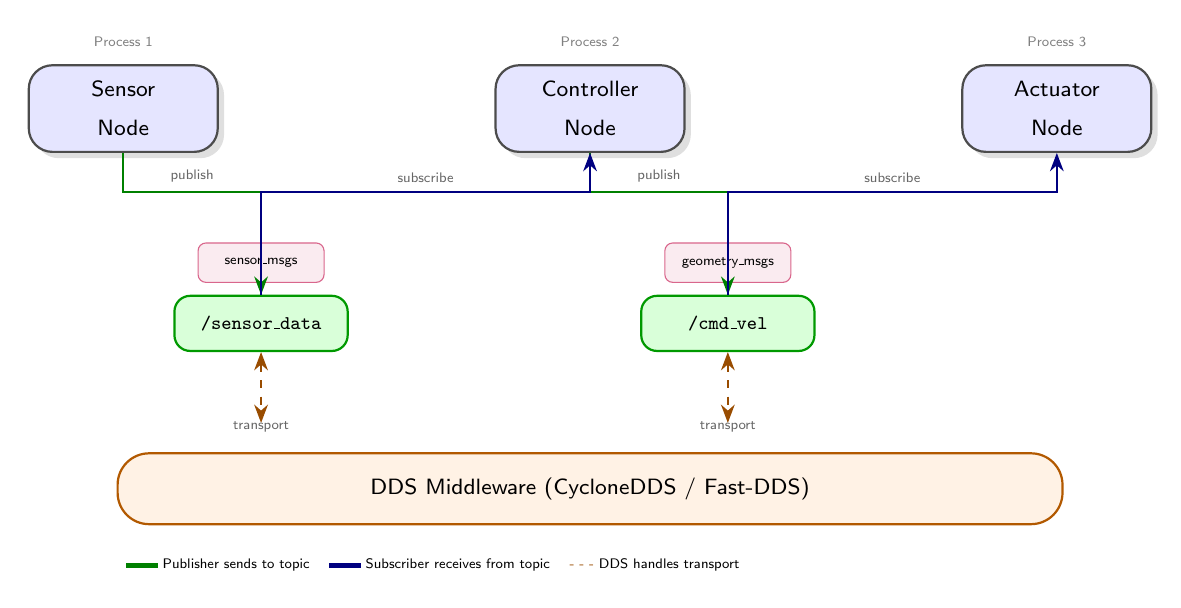
\begin{tikzpicture}[
    node distance=1.2cm and 2.5cm,
    % Node style (ROS 2 computational units)
    rosnode/.style={
        draw=black!70,
        rounded corners=3mm,
        minimum width=2.4cm,
        minimum height=1.1cm,
        font=\sffamily\footnotesize,
        fill=blue!10,
        thick,
        align=center,
        drop shadow={opacity=0.25, shadow xshift=0.08cm, shadow yshift=-0.08cm}
    },
    % Topic style (communication channels)
    topic/.style={
        draw=green!60!black,
        rounded corners=2mm,
        minimum width=2.2cm,
        minimum height=0.7cm,
        font=\sffamily\scriptsize\ttfamily,
        fill=green!15,
        thick,
        align=center
    },
    % DDS layer style
    dds/.style={
        draw=orange!70!black,
        rounded corners=4mm,
        minimum height=0.9cm,
        font=\sffamily\footnotesize,
        fill=orange!10,
        thick,
        align=center
    },
    % Message style
    msg/.style={
        draw=purple!60,
        rounded corners=1mm,
        minimum width=1.6cm,
        minimum height=0.5cm,
        font=\sffamily\tiny,
        fill=purple!8,
        align=center
    },
    % Arrow styles
    pub arrow/.style={->, >=Stealth, thick, color=green!50!black},
    sub arrow/.style={<-, >=Stealth, thick, color=blue!50!black},
    dds arrow/.style={<->, >=Stealth, thick, color=orange!60!black, dashed},
    % Labels
    label/.style={font=\sffamily\tiny, color=black!60}
]

% === ROS 2 Nodes ===
\node[rosnode] (sensor) {Sensor\\Node};
\node[rosnode, right=3.5cm of sensor] (controller) {Controller\\Node};
\node[rosnode, right=3.5cm of controller] (actuator) {Actuator\\Node};

% === Topics (between nodes) ===
\node[topic, below=1.8cm of sensor, xshift=1.75cm] (topic1) {/sensor\_data};
\node[topic, below=1.8cm of controller, xshift=1.75cm] (topic2) {/cmd\_vel};

% === Message types ===
\node[msg, above=0.15cm of topic1] (msg1) {sensor\_msgs};
\node[msg, above=0.15cm of topic2] (msg2) {geometry\_msgs};

% === DDS Layer ===
\node[dds, below=3.8cm of controller, minimum width=12cm] (dds)
    {DDS Middleware (CycloneDDS / Fast-DDS)};

% === Publish arrows ===
\draw[pub arrow] (sensor.south) -- ++(0,-0.5) -| node[label, pos=0.25, above] {publish} (topic1.north);
\draw[pub arrow] (controller.south) -- ++(0,-0.5) -| node[label, pos=0.25, above] {publish} (topic2.north);

% === Subscribe arrows ===
\draw[sub arrow] (controller.south) -- ++(0,-0.5) -| node[label, pos=0.25, above] {subscribe} (topic1.north);
\draw[sub arrow] (actuator.south) -- ++(0,-0.5) -| node[label, pos=0.25, above] {subscribe} (topic2.north);

% === DDS connections ===
\draw[dds arrow] (topic1.south) -- ++(0,-0.6) -- node[label, below, pos=0.5] {transport} ++(0,-0.3);
\draw[dds arrow] (topic2.south) -- ++(0,-0.6) -- node[label, below, pos=0.5] {transport} ++(0,-0.3);

% === Legend ===
\node[below=0.3cm of dds.south west, anchor=north west, font=\sffamily\tiny, align=left] (legend) {
    \textcolor{green!50!black}{\rule{0.4cm}{2pt}} Publisher sends to topic \quad
    \textcolor{blue!50!black}{\rule{0.4cm}{2pt}} Subscriber receives from topic \quad
    \textcolor{orange!60!black}{- - -} DDS handles transport
};

% === Annotations ===
\node[font=\sffamily\tiny, color=black!50, above=0.1cm of sensor.north] {Process 1};
\node[font=\sffamily\tiny, color=black!50, above=0.1cm of controller.north] {Process 2};
\node[font=\sffamily\tiny, color=black!50, above=0.1cm of actuator.north] {Process 3};

\end{tikzpicture}
\caption[ROS 2 pub-sub architecture]{ROS 2 publish-subscribe architecture. Nodes are independent processes that communicate through typed topics. Publishers send messages without knowledge of subscribers, and subscribers receive messages without knowledge of publishers. The DDS middleware layer handles discovery, serialization, and transport, enabling distributed communication with configurable quality-of-service policies.}
\label{fig:ros2_architecture}
\end{figure}

Communication occurs through typed topics: publishers send messages to named topics while subscribers receive those messages, with DDS handling transport, discovery, and quality-of-service enforcement. Message types follow standardized definitions (e.g., \texttt{sensor\_msgs/JointState}, \texttt{nav\_msgs/Odometry}, \texttt{geometry\_msgs/Twist}) ensuring interoperability across platforms and vendors. Quality-of-service policies control reliability (reliable vs. best-effort delivery), durability (transient vs. volatile message retention), history depth (number of messages buffered), and deadline constraints (maximum acceptable time between messages).

Unitree humanoid robots employ specific ROS 2 communication patterns that any validation framework must replicate. The \texttt{/lowstate} topic publishes joint positions, velocities, torques, and IMU data at 500-1000 Hz, providing high-frequency proprioceptive feedback. The \texttt{/lowcmd} topic subscribes to joint position or torque commands at matching frequencies, enabling low-level motor control. Sensor topics such as \texttt{/utlidar/cloud} publish 3D LiDAR point clouds at 10 Hz, while camera topics provide RGB-D images for perception tasks. This multi-rate communication structure requires careful temporal synchronization to maintain control stability.

\textcite{digitaltwinros2023development} demonstrate ROS-based digital twin implementations for mobile robots, emphasizing the importance of authentic communication protocols for credible validation. Their work shows that digital twins employing actual ROS messaging exhibit more realistic behavior than those using direct function calls, as the communication layer introduces latencies, buffering effects, and serialization overheads characteristic of deployed systems.

This thesis leverages ROS 2 Humble (the long-term support release with maintenance through 2027) with CycloneDDS middleware to implement communication-realistic validation. By replicating Unitree-compatible topic structures, message types, and publication frequencies in simulation, the framework enables policies to be evaluated under authentic communication constraints before physical deployment. This approach addresses the communication validation gap identified in existing sim-to-real methodologies, providing an intermediate verification step that assesses policy performance under realistic message passing patterns, latencies, and asynchronous transport characteristics.

\subsection{Research Gaps and Thesis Positioning}

Consider a typical educational robotics laboratory where a single \$20,000 Unitree G1 humanoid robot must serve thousands of students across multiple years. Existing sim-to-real methodologies train policies with domain randomization and deploy directly to physical hardware \parencite{gu2024humanoidgym}, treating hardware as the first validation under real-world conditions. If the policy fails—due to insufficient randomization, unmodeled dynamics, or communication issues—the robot falls, potentially damaging expensive actuators or structural components. The educational program stalls while repairs are completed or replacement hardware is procured, denying hundreds of students access to hands-on robotics research.

This scenario reveals critical gaps in current humanoid locomotion research: the lack of credible intermediate validation before physical deployment, the assumption of ready hardware access for iterative testing, and the absence of communication-realistic verification despite real robots operating through middleware frameworks like ROS 2. Educational institutions cannot afford the risks inherent in direct sim-to-real transfer, yet state-of-the-art alternatives demand resources beyond typical budgets—transformer-based methods require hundreds of GPUs for weeks \parencite{radosavovic2024realworld}, while motion capture approaches need specialized laboratory infrastructure \parencite{cheng2024expressive}.

This thesis addresses these gaps through an integrated framework combining novel task design, communication-realistic validation, and accessible deployment strategies. Rather than listing contributions abstractly, this section demonstrates how the work extends existing methodologies to serve educational contexts where hardware access is severely constrained.

\subsubsection{End-to-End Point-to-Point Navigation via Low-Level Joint Control}

Traditional approaches to humanoid navigation employ hierarchical architectures: a high-level planner generates waypoints or footstep plans, a mid-level controller computes joint trajectories, and a low-level controller tracks those trajectories \parencite{cheng2024expressive}. This decomposition simplifies the problem but introduces challenges: trajectory optimization becomes computationally expensive, footstep planning requires accurate terrain models, and coordination between hierarchy levels demands careful tuning. Each abstraction layer accumulates errors and delays, potentially degrading performance.

This work adopts a fundamentally different strategy: end-to-end point-to-point navigation through direct reinforcement learning of low-level joint control across 29 degrees of freedom. The policy receives goal positions and current robot state, then directly outputs joint position targets without intermediate trajectory generation or footstep planning. This approach eliminates hierarchical abstractions, enabling the policy to discover efficient locomotion strategies through environmental interaction rather than relying on hand-engineered motion primitives. The choice of end-to-end learning over hierarchical decomposition is deliberate: while hierarchical architectures can provide interpretable intermediate representations and may facilitate modular development, recent work in legged robotics has demonstrated that end-to-end approaches achieve competitive or superior performance while substantially reducing engineering complexity \parencite{gu2024humanoidgym}. For educational contexts where maintainability and reproducibility are paramount, architectural simplicity provides significant advantages.

The benefits prove substantial. Training becomes simpler: a single neural network replaces multiple coordinated controllers, reducing architectural complexity and hyperparameter tuning. The policy learns adaptive behaviors: rather than following pre-computed trajectories, the controller continuously adjusts joint commands based on current state, enabling reactive responses to disturbances. Computational efficiency improves: inference requires a single forward pass through a compact network (typically 256-512 hidden units) rather than solving optimization problems or computing inverse kinematics at each timestep. Most critically, the learned behaviors often surpass hand-engineered approaches in robustness, as the policy experiences diverse randomized conditions during training and develops strategies that generalize across parameter variations.

Key design innovations enable this end-to-end approach. Forward-biased goal sampling places navigation targets ahead of the robot rather than uniformly around it, encouraging forward locomotion rather than stationary pivoting. Heading-aware velocity scaling adjusts commanded forward velocity based on angular alignment with the goal: when facing the target, maximum forward speed is permitted; when misaligned, rotational correction takes priority. Distance-adaptive speed control increases velocity as goals approach, enabling both long-range traversal and precise terminal positioning. Graduated reward shaping balances competing objectives—goal achievement, locomotion smoothness, energy efficiency, and stability—through carefully weighted terms that guide policy learning without over-constraining exploration.

This methodology extends the Humanoid-Gym framework \parencite{gu2024humanoidgym}, which demonstrated velocity-tracking locomotion but not goal-directed navigation. By transforming low-level joint control from velocity tracking to spatial navigation, this work enables autonomous robot operation suitable for real-world tasks: delivering objects to specified locations, patrolling designated waypoints, or approaching users who request assistance. The approach remains accessible—training completes in 3-4 hours on a single NVIDIA RTX 4080 GPU—while providing capabilities previously requiring hierarchical architectures or expensive motion planning infrastructure.

Figure \ref{fig:architecture_comparison} illustrates this architectural distinction, contrasting traditional hierarchical decomposition with the end-to-end approach adopted in this work.

\begin{figure}[H]
\centering
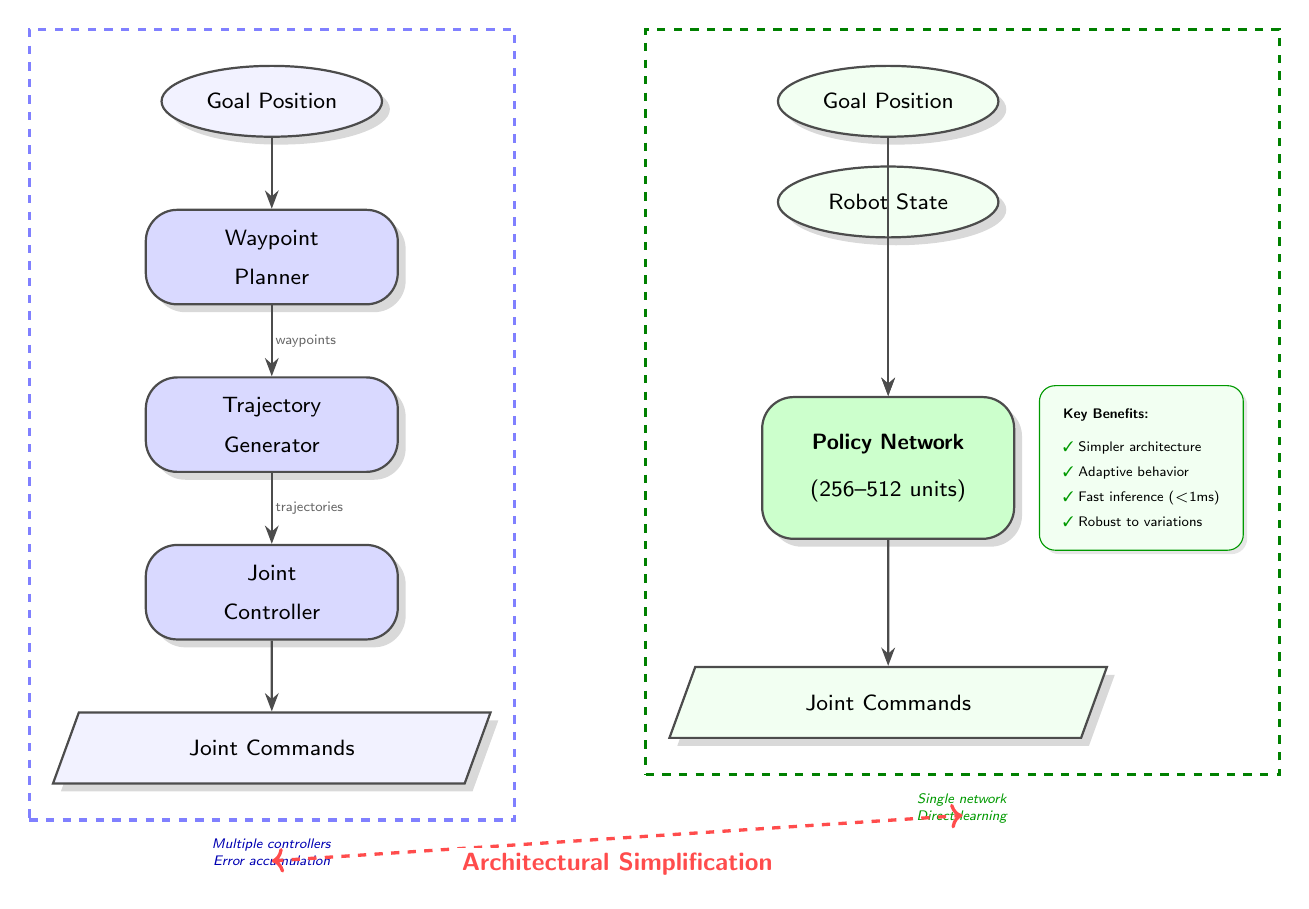
\begin{tikzpicture}[
    node distance=1cm and 3cm,
    % Enhanced module style with shadows
    module/.style={
        draw=black!70,
        rounded corners=4mm,
        minimum width=3.2cm,
        minimum height=1.2cm,
        font=\sffamily\footnotesize,
        fill=white,
        thick,
        align=center,
        drop shadow={opacity=0.3, shadow xshift=0.1cm, shadow yshift=-0.1cm}
    },
    % Enhanced input style
    input/.style={
        draw=black!70,
        ellipse,
        minimum width=2.8cm,
        minimum height=0.9cm,
        font=\sffamily\footnotesize,
        fill=white,
        thick,
        align=center,
        drop shadow={opacity=0.3, shadow xshift=0.1cm, shadow yshift=-0.1cm}
    },
    % Enhanced output style
    output/.style={
        draw=black!70,
        trapezium,
        trapezium left angle=70,
        trapezium right angle=110,
        minimum width=2.8cm,
        minimum height=0.9cm,
        font=\sffamily\footnotesize,
        fill=white,
        thick,
        align=center,
        drop shadow={opacity=0.3, shadow xshift=0.1cm, shadow yshift=-0.1cm}
    },
    % Arrow styles
    arrow/.style={->, >=Stealth, thick, color=black!70},
    arrow label/.style={font=\sffamily\tiny, color=black!60, midway, fill=white, inner sep=1pt},
    % Label and box styles
    label/.style={font=\sffamily\bfseries\normalsize},
    benefit box/.style={
        draw=green!60!black,
        rounded corners=2mm,
        fill=green!5,
        align=left,
        font=\sffamily\tiny,
        inner sep=0.3cm,
        drop shadow={opacity=0.2, shadow xshift=0.05cm, shadow yshift=-0.05cm}
    }
]

% Traditional Hierarchical Architecture (Left Side)
\node[input, fill=blue!5] (h_input) {Goal Position};
\node[module, below=0.9cm of h_input, fill=blue!15] (h_planner) {Waypoint\\Planner};
\node[module, below=0.9cm of h_planner, fill=blue!15] (h_traj) {Trajectory\\Generator};
\node[module, below=0.9cm of h_traj, fill=blue!15] (h_ctrl) {Joint\\Controller};
\node[output, below=0.9cm of h_ctrl, fill=blue!5] (h_output) {Joint Commands};

% Arrows for hierarchical with labels
\draw[arrow] (h_input) -- (h_planner);
\draw[arrow] (h_planner) -- node[arrow label, right] {waypoints} (h_traj);
\draw[arrow] (h_traj) -- node[arrow label, right] {trajectories} (h_ctrl);
\draw[arrow] (h_ctrl) -- (h_output);

% Bounding box for hierarchical
\node[draw=blue!50, dashed, very thick, fit=(h_input) (h_output), inner sep=0.45cm,
      label={[label, color=blue!70!black]above:Traditional Hierarchical}] (box_h) {};

% Add complexity annotation
\node[font=\sffamily\tiny, color=blue!70!black, below=0.1cm of box_h.south, align=center]
    {\textit{Multiple controllers}\\[-1mm]\textit{Error accumulation}};

% End-to-End Architecture (Right Side)
\node[input, right=5cm of h_input, fill=green!5] (e_input1) {Goal Position};
\node[input, below=0.35cm of e_input1, fill=green!5] (e_input2) {Robot State};
\node[module, below=2.0cm of e_input2, fill=green!20, minimum height=1.8cm, text width=2.8cm] (e_policy) {
    \textbf{Policy Network}\\[1mm]
    {\footnotesize (256--512 units)}
};
\node[output, below=1.6cm of e_policy, fill=green!5] (e_output) {Joint Commands};

% Arrows for end-to-end
\draw[arrow] (e_input1.south) -- ++(0,-0.15) -| (e_policy.north -| e_input1);
\draw[arrow] (e_input2.south) -- (e_policy.north -| e_input2);
\draw[arrow] (e_policy) -- (e_output);

% Enhanced benefits box
\node[benefit box, right=0.3cm of e_policy] (benefits) {
    \textbf{Key Benefits:}\\[1mm]
    \textcolor{green!60!black}{\cmark} Simpler architecture\\
    \textcolor{green!60!black}{\cmark} Adaptive behavior\\
    \textcolor{green!60!black}{\cmark} Fast inference ($<$1ms)\\
    \textcolor{green!60!black}{\cmark} Robust to variations
};

% Bounding box for end-to-end
\node[draw=green!50!black, dashed, very thick, fit=(e_input1) (e_output) (benefits), inner sep=0.45cm,
      label={[label, color=green!60!black]above:End-to-End (This Work)}] (box_e) {};

% Add simplicity annotation
\node[font=\sffamily\tiny, color=green!60!black, below=0.1cm of box_e.south, align=center]
    {\textit{Single network}\\[-1mm]\textit{Direct learning}};

% Comparison arrow with better styling
\draw[<->, very thick, dashed, red!70, line width=1.2pt]
    ([yshift=-0.5cm]box_h.south) --
    node[below=1mm, font=\sffamily\small\bfseries, color=red!70, fill=white, inner sep=2pt]
    {Architectural Simplification}
    ([yshift=-0.5cm]box_e.south);

\end{tikzpicture}
\caption[Hirearchical Navigation vs End-to-End approach]{Comparison of traditional hierarchical navigation architecture versus the end-to-end approach adopted in this work. The hierarchical architecture requires multiple coordinated controllers and intermediate representations (waypoints, trajectories), accumulating errors and computational costs. The end-to-end approach directly maps goal positions and robot state to joint commands through a single learned policy, eliminating abstraction layers while achieving superior robustness through diverse training experiences.}
\label{fig:architecture_comparison}
\end{figure}

\subsubsection{Communication-Realistic Validation Through Authentic ROS 2 Middleware}

With a navigation policy trained through domain randomization, existing methodologies proceed directly to physical deployment \parencite{gu2024humanoidgym}. The policy has experienced physics variations—randomized masses, friction coefficients, joint damping—but has never encountered communication constraints present in real robotic systems. During training and pure-simulation validation, the policy receives observations through direct Python function calls with nanosecond latencies. During physical deployment, observations flow through ROS 2 topics, with serialization overheads, network transport latencies (1-10ms), and asynchronous publishing creating temporal misalignment between sensor measurements and control decisions.

This communication gap could degrade performance or introduce instability. Consider a humanoid maintaining balance: if expected joint state observations arrive 5ms late due to middleware latency, the policy's learned control strategy—tuned for instantaneous feedback during training—might generate inappropriate commands, destabilizing the robot. Policies validated only in pure simulation have no opportunity to develop robustness to these timing characteristics before encountering them on expensive hardware.

This thesis introduces simulation-to-simulation validation employing authentic ROS 2 Humble communication protocols as an intermediate verification step. A second simulation environment implements the complete middleware stack: Unitree-compatible topics (\texttt{/lowstate} for proprioceptive sensing, \texttt{/lowcmd} for motor commands, \texttt{/utlidar/cloud} for LiDAR perception), realistic publication frequencies (50 Hz for joint states, 10 Hz for point clouds), message serialization through standard ROS 2 types (\texttt{sensor\_msgs/JointState}, \texttt{nav\_msgs/Odometry}), and DDS transport introducing characteristic latencies and asynchronous delivery patterns.

Policies trained in Isaac Lab deploy to this communication-realistic environment before physical hardware testing. If the policy maintains stable locomotion and achieves navigation goals under ROS 2 constraints, confidence in hardware deployment increases substantially. If communication latencies cause instability or degraded performance, these issues surface in simulation where debugging incurs no hardware damage risks. This staged validation—physics-based training with domain randomization, followed by communication-realistic evaluation with authentic middleware—provides two verification stages before requesting precious physical robot time.

The framework replicates communication constraints present in real Unitree robots. The \texttt{/lowstate} topic publishes 29-DOF joint positions and velocities, alog 6-DOF IMU data, matching Unitree SDK2 message structures. Commands flow through \texttt{/lowcmd} topics using position-control or torque-control modes, respecting actuator bandwidth limitations. Temporal synchronization employs ROS 2 clock mechanisms (\texttt{/clock} topic) ensuring consistent timestamps across distributed nodes. Quality-of-service policies match real-world configurations: reliable delivery for control commands (cannot afford message loss), and best-effort for high-frequency sensor streams (latest measurement matters more than historical completeness).

This approach addresses the communication validation gap identified in existing sim-to-sim transfer research. While prior work validates policies across different physics engines \parencite{gu2024humanoidgym}, it typically ignores middleware realism, evaluating policies through direct simulator function calls. By introducing authentic ROS 2 communication as an intermediate validation layer, this work provides credible assessment of policy readiness before physical deployment—particularly valuable for educational contexts where hardware damage risks must be minimized.

\subsubsection{Educational Accessibility Through Containerized Deployment}

The validation framework proves most valuable when accessible to students with limited computational resources and no physical robot access. This thesis packages the complete system—Isaac Sim 4.5, Isaac Lab 2.2, ROS 2 Humble, CycloneDDS middleware, trained policy checkpoints, and all dependencies—into Docker containers with reproducible multi-stage builds. Students clone a repository, execute a single build command, and obtain a complete training and validation environment without manual dependency resolution or version conflicts.

This containerization strategy addresses educational access barriers identified in the literature. Transformer-based approaches \parencite{radosavovic2024realworld} require massive GPU clusters, which are unavailable to most students. Motion capture methods \parencite{cheng2024expressive} demand specialized laboratory infrastructure. Iterative sim-to-real validation assumes ready hardware access for testing. In contrast, this framework enables students to develop, train, and validate locomotion policies entirely in simulation on personal workstations or shared university servers. They progress through physics-based training (requiring GPU resources but no hardware access) and communication-realistic validation (introducing ROS 2 constraints) before requesting physical robot time.

The educational benefits extend beyond hardware preservation. Students gain hands-on experience with industrial-standard tools: ROS 2 for robotics middleware, Docker for reproducible deployment, Isaac Lab for GPU-accelerated simulation, and PPO for policy optimization. They iterate rapidly—training a policy in 6-8 hours, evaluating in sim-to-sim validation immediately, then refining based on observed behaviors—without scheduling physical robot access or risking expensive hardware during exploratory experiments. When confident in policy performance through two simulation-based verification stages, they request robot time for final validation, maximizing learning opportunities while minimizing hardware risks.

This approach enables students to engage with humanoid robotics research using shared physical resources. A single university robot serves an entire graduate program: students develop policies independently in simulation, demonstrate successful sim-to-sim validation to instructors, then receive supervised robot access for final verification. This staged progression from pure simulation, through communication-realistic validation, to physical deployment balances educational accessibility with research rigor.

\subsubsection{Positioning and Future Validation}

This thesis adopts direct reinforcement learning for its accessibility, reproducibility, and proven transferability \parencite{gu2024humanoidgym}, but diverges from existing frameworks through staged validation and educational focus. The ultimate validation remains sim-to-real transfer to physical Unitree G1 hardware (Phase 7, future work beyond this thesis scope). However, by providing two simulation-based verification stages before physical deployment, this work enables safer progression toward hardware testing particularly suitable for educational contexts where thousands of students must share limited resources.

Future work will assess whether communication-realistic sim-to-sim validation improves first-deployment success rates and reduces hardware damage incidents compared to direct sim-to-real approaches. Preliminary sim-to-sim results demonstrate successful policy operation under authentic ROS 2 constraints, providing encouraging evidence for eventual physical transfer while maintaining the educational accessibility that motivated this research. The framework positions simulation-to-simulation validation not as a replacement for physical deployment but as a credible intermediate step that increases deployment confidence and reduces iteration costs for resource-constrained educational institutions.


\newpage

\section{Problem Formulation}

This section formalizes the humanoid locomotion control problem as a Markov Decision Process (MDP), providing the mathematical foundation for the reinforcement learning approach developed in subsequent chapters. The formal specification enables precise discussion of state representations, action spaces, reward structures, and optimization objectives.

\subsection{Markov Decision Process Formulation}

The goal-directed locomotion task is formulated as a finite-horizon MDP defined by the tuple $\mathcal{M} = (\mathcal{S}, \mathcal{A}, P, R, \gamma, T)$, where $\mathcal{S}$ denotes the state space, $\mathcal{A}$ the action space, $P$ the transition dynamics, $R$ the reward function, $\gamma$ the discount factor, and $T$ the episode horizon.

\subsubsection{State Space $\mathcal{S}$}

The state space $\mathcal{S} \subseteq \mathbb{R}^{n_s}$ comprises proprioceptive observations available to the policy. For the base locomotion task, $n_s = 125$:

\begin{equation}
\mathbf{s}_t = \left[ \mathbf{p}_{goal}^{base}, \mathbf{v}_{base}, \boldsymbol{\omega}_{base}, \mathbf{g}_{proj}, \mathbf{q}, \dot{\mathbf{q}}, \mathbf{v}_{cmd}, \mathbf{a}_{t-1} \right]^\top
\label{eq:state_vector}
\end{equation}

Table \ref{tab:state_space} details each component of the state vector.

\begin{table}[H]
\centering
\caption{State space components for base locomotion task}
\label{tab:state_space}
\footnotesize
\begin{tabular}{l|c|l}
\toprule
\textbf{Component} & \textbf{Dimension} & \textbf{Description} \\
\midrule
$\mathbf{p}_{goal}^{base}$ & 2 & Goal position in base frame $(x, y)$ \\
$\mathbf{v}_{base}$ & 3 & Base linear velocity $(v_x, v_y, v_z)$ \\
$\boldsymbol{\omega}_{base}$ & 3 & Base angular velocity $(\omega_x, \omega_y, \omega_z)$ \\
$\mathbf{g}_{proj}$ & 3 & Projected gravity vector (orientation encoding) \\
$\mathbf{q}$ & 29 & Joint positions (radians) \\
$\dot{\mathbf{q}}$ & 29 & Joint velocities (rad/s) \\
$\mathbf{v}_{cmd}$ & 3 & Velocity commands $(v_x^{cmd}, v_y^{cmd}, \omega_z^{cmd})$ \\
$\mathbf{a}_{t-1}$ & 29 & Previous actions \\
\midrule
\textbf{Total} & \textbf{125} & \\
\bottomrule
\end{tabular}
\end{table}

For the social navigation variant, the state space extends to $\mathcal{S} \subseteq \mathbb{R}^{141}$ with additional LiDAR sector observations $\mathbf{l} \in \mathbb{R}^{16}$:

\begin{equation}
\mathbf{s}_t^{social} = \left[ \mathbf{s}_t, \mathbf{l}_t \right]^\top, \quad l_i = \frac{\min(d_i, d_{max})}{d_{max}} \in [0, 1]
\end{equation}

where $l_i$ represents the normalized minimum distance to any obstacle within the $i$-th angular sector (each spanning $22.5\circ$), and $d_{max} = 10$ m is the maximum LiDAR range. The state representation uses proprioceptive observations rather than privileged simulator state, ensuring policies can execute on physical hardware.

\subsubsection{Action Space $\mathcal{A}$}

The action space $\mathcal{A} \subseteq \mathbb{R}^{29}$ consists of target joint position offsets from a default standing pose $\mathbf{q}_{default}$:

\begin{equation}
\mathbf{a}_t = \Delta\mathbf{q}_{target} \in [-1, 1]^{29}
\label{eq:action_space}
\end{equation}

Actions are scaled by joint-specific position limits and converted to target positions:

\begin{equation}
q_{target,j} = q_{default,j} + a_j \cdot \Delta q_{max,j}
\end{equation}

where $\Delta q_{max,j}$ defines the maximum position deviation for joint $j$. A proportional-derivative (PD) controller converts position targets to joint torques:

\begin{equation}
\tau_j = K_p (q_{target,j} - q_j) + K_d (\dot{q}_{target,j} - \dot{q}_j)
\label{eq:pd_control}
\end{equation}

with gains $K_p = 50$ N$\cdot$m/rad and $K_d = 1$ N$\cdot$m$\cdot$s/rad, matching Unitree G1 default parameters. Position-based actions with PD control match the interface available on physical Unitree robots and provide implicit compliance for contact stability.

\subsubsection{Transition Dynamics $P$}

The transition function $P: \mathcal{S} \times \mathcal{A} \rightarrow \Delta(\mathcal{S})$ maps state-action pairs to probability distributions over next states. The dynamics are defined implicitly through physics simulation:

\begin{equation}
\mathbf{s}_{t+1} \sim P(\cdot | \mathbf{s}_t, \mathbf{a}_t) = \text{PhysX}(\mathbf{s}_t, \mathbf{a}_t, \boldsymbol{\xi}_t)
\label{eq:transition}
\end{equation}

where PhysX denotes the NVIDIA PhysX 5 simulation engine, and $\boldsymbol{\xi}_t$ represents stochastic elements introduced through domain randomization. Table \ref{tab:domain_randomization} specifies the randomization distributions.

\begin{table}[H]
\centering
\caption{Domain randomization parameters}
\label{tab:domain_randomization}
\footnotesize
\begin{tabular}{l|c|l}
\toprule
\textbf{Parameter} & \textbf{Distribution} & \textbf{Rationale} \\
\midrule
Link masses & $\mathcal{U}[0.85m, 1.15m]$ & Manufacturing tolerances, payload variation \\
Ground friction & $\mathcal{U}[0.5, 1.2]$ & Surface material variation \\
Joint damping & $\mathcal{U}[0.8d, 1.2d]$ & Actuator wear, temperature effects \\
Motor strength & $\mathcal{U}[0.9\tau, 1.1\tau]$ & Battery voltage, motor efficiency \\
Observation noise & $\mathcal{N}(0, \sigma_q^2)$, $\sigma_q = 0.01$ rad & Encoder noise \\
Action delay & $\mathcal{U}\{1, 2, 3\}$ steps & Communication latency \\
\bottomrule
\end{tabular}
\end{table}

These ranges derive from common practice in legged robotics \parencite{gu2024humanoidgym, hwangbo2019learning} and approximate expected hardware variation.

\subsubsection{Reward Function $R$}

The reward function $R: \mathcal{S} \times \mathcal{A} \rightarrow \mathbb{R}$ is a weighted combination of task objectives and regularization terms:

\begin{equation}
R(\mathbf{s}_t, \mathbf{a}_t) = \sum_{i=1}^{N} w_i \cdot r_i(\mathbf{s}_t, \mathbf{a}_t)
\label{eq:reward_function}
\end{equation}

Table \ref{tab:reward_specification} provides the complete reward specification, including mathematical definitions for the base locomotion task.

\begin{table}[H]
\centering
\caption{Reward function specification for base locomotion}
\label{tab:reward_specification}
\footnotesize
\begin{tabular}{l|c|p{6cm}}
\toprule
\textbf{Term} & \textbf{Weight} & \textbf{Mathematical Definition} \\
\midrule
\multicolumn{3}{l}{\textit{Task Objectives}} \\
\midrule
Linear velocity tracking & 1.0 & $r_{vel} = \exp\left(-\|\mathbf{v}_{xy} - \mathbf{v}_{xy}^{cmd}\|^2 / \sigma_{vel}^2\right)$, $\sigma_{vel} = 0.25$ \\
Angular velocity tracking & 1.0 & $r_{\omega} = \exp\left(-(\omega_z - \omega_z^{cmd})^2 / \sigma_{\omega}^2\right)$, $\sigma_{\omega} = 0.25$ \\
Goal distance (coarse) & 0.3 & $r_{goal,c} = \exp\left(-d_{goal}^2 / \sigma_c^2\right)$, $\sigma_c = 5.0$ \\
Goal distance (fine) & 0.2 & $r_{goal,f} = \exp\left(-d_{goal}^2 / \sigma_f^2\right)$, $\sigma_f = 3.0$ \\
Heading alignment & 0.3 & $r_{head} = \exp\left(-\theta_{error}^2 / \sigma_h^2\right)$, $\sigma_h = 0.5$ \\
Feet air time & 0.75 & $r_{air} = \sum_{i \in feet} \max(0, t_{air,i} - 0.1)$ \\
\midrule
\multicolumn{3}{l}{\textit{Regularization (Penalties)}} \\
\midrule
Action rate & $-0.005$ & $r_{act} = -\|\mathbf{a}_t - \mathbf{a}_{t-1}\|^2$ \\
Joint deviation (arms) & $-0.1$ & $r_{joint} = -\|\mathbf{q}_{arms} - \mathbf{q}_{default,arms}\|^2$ \\
Feet slide & $-0.1$ & $r_{slide} = -\sum_{i \in feet} \|\mathbf{v}_{foot,i}\| \cdot c_i$ \\
Flat orientation & $-1.0$ & $r_{flat} = -\|\mathbf{g}_{proj,xy}\|^2$ \\
Backwards velocity & $-0.5$ & $r_{back} = -\mathbb{1}[v_x < -0.1]$ \\
Termination & $-200$ & $r_{term} = -\mathbb{1}[\text{fall}]$ \\
\bottomrule
\end{tabular}
\end{table}

The exponential kernel form $\exp(-x^2/\sigma^2)$ provides smooth gradients for optimization. The dual goal rewards address sparsity: coarse ($\sigma = 5.0$) provides long-range gradient, fine ($\sigma = 3.0$) enables precise positioning.

\subsubsection{Discount Factor and Episode Horizon}

The discount factor $\gamma = 0.99$ balances immediate and future rewards, with effective horizon $\frac{1}{1-\gamma} = 100$ steps. Episodes terminate after $T = 1000$ steps (20 seconds at 50 Hz control frequency) or upon early termination conditions:

\begin{itemize}
    \item \textbf{Base contact:} Any non-foot body part contacts the ground (fall detection)
    \item \textbf{Height violation:} Base height falls below threshold ($z_{base} < 0.3$ m)
    \item \textbf{Orientation violation:} Excessive body tilt ($|\theta_{roll}| > 1.0$ rad or $|\theta_{pitch}| > 1.0$ rad)
\end{itemize}

Early termination triggers the termination penalty ($r_{term} = -200$), providing strong gradient against unsafe states.

\subsection{Optimization Objective}

The objective is to find a policy $\pi_\theta: \mathcal{S} \rightarrow \Delta(\mathcal{A})$ parameterized by neural network weights $\theta$ that maximizes expected cumulative discounted reward:

\begin{equation}
\pi^* = \arg\max_{\pi_\theta} J(\theta) = \arg\max_{\pi_\theta} \mathbb{E}_{\tau \sim \pi_\theta} \left[ \sum_{t=0}^{T} \gamma^t R(\mathbf{s}_t, \mathbf{a}_t) \right]
\label{eq:objective}
\end{equation}

where $\tau = (\mathbf{s}_0, \mathbf{a}_0, r_0, \mathbf{s}_1, \mathbf{a}_1, r_1, \ldots)$ denotes a trajectory sampled under policy $\pi_\theta$, with initial states drawn from distribution $\mathbf{s}_0 \sim \rho_0$.

The policy $\pi_\theta(\mathbf{a}|\mathbf{s})$ is represented as a diagonal Gaussian distribution:

\begin{equation}
\pi_\theta(\mathbf{a}|\mathbf{s}) = \mathcal{N}(\boldsymbol{\mu}_\theta(\mathbf{s}), \text{diag}(\boldsymbol{\sigma}_\theta^2))
\label{eq:policy_distribution}
\end{equation}

where the mean $\boldsymbol{\mu}_\theta(\mathbf{s}) \in \mathbb{R}^{29}$ is output by the actor network, and the standard deviation $\boldsymbol{\sigma}_\theta \in \mathbb{R}^{29}$ is learned as state-independent parameters. During training, actions are sampled from this distribution to enable exploration; during evaluation, the deterministic mean $\boldsymbol{\mu}_\theta(\mathbf{s})$ is typically used.

\subsection{Problem Characteristics and Algorithm Selection}

The MDP exhibits characteristics that motivate algorithm selection: high-dimensional continuous state ($\mathbb{R}^{125}$) and action ($\mathbb{R}^{29}$) spaces requiring function approximation; partial observability (proprioceptive observations only); stochastic dynamics from domain randomization; and real-time execution constraints (50 Hz, requiring sub-millisecond inference).

Proximal Policy Optimization (PPO) \parencite{schulman2017proximal} was selected based on: (1) stability through trust region constraints, critical for safety-sensitive robotics; (2) proven sim-to-real transfer on Unitree platforms \parencite{gu2024humanoidgym} and ANYmal \parencite{hwangbo2019learning}; (3) effective parallelization enabling 100,000+ transitions/second with 512 environments; and (4) mature RSL-RL implementation optimized for Isaac Lab. Alternative algorithms (SAC, TD3) were not evaluated; comparative studies remain for future work.

\newpage

\section{Methodology}

This thesis employs a phased methodology that progresses from environment creation through policy training to communication-realistic validation. The approach addresses three interconnected challenges: creating a high-fidelity simulation environment that accurately represents the physical deployment context, training locomotion policies capable of goal-directed navigation through low-level joint control, and validating those policies under realistic communication constraints before physical deployment. Figure \ref{fig:methodology_overview} illustrates the complete methodological pipeline, showing data flow between phases and the progressive refinement from pure simulation toward deployment readiness.

\begin{figure}[H]
\centering
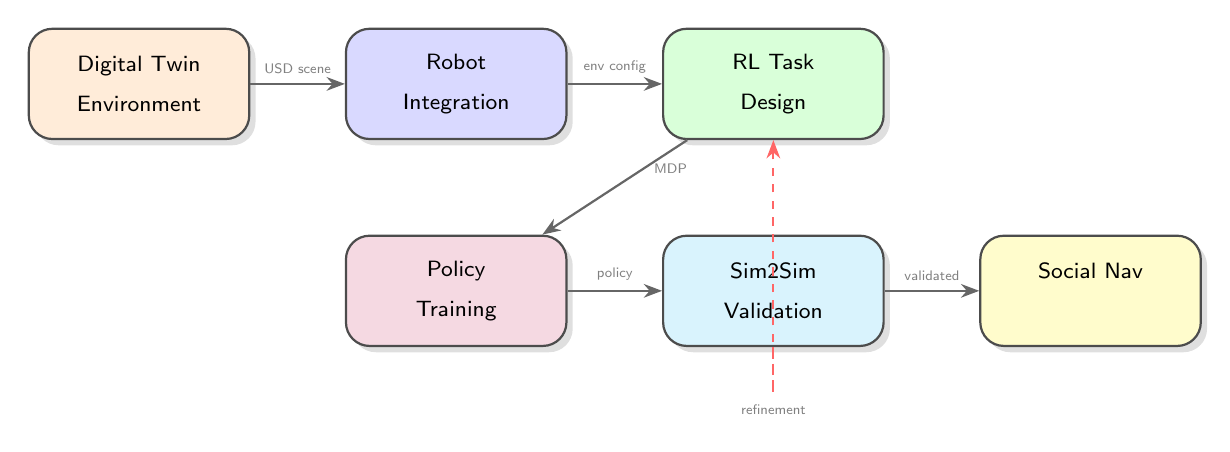
\begin{tikzpicture}[
    node distance=0.8cm and 1.5cm,
    phase/.style={
        draw=black!70,
        rounded corners=3mm,
        minimum width=2.8cm,
        minimum height=1.4cm,
        font=\sffamily\footnotesize,
        fill=white,
        thick,
        align=center,
        drop shadow={opacity=0.25, shadow xshift=0.08cm, shadow yshift=-0.08cm}
    },
    arrow/.style={->, >=Stealth, thick, color=black!60},
    label/.style={font=\sffamily\tiny, color=black!50}
]

\node[phase, fill=orange!15] (p1) {Digital Twin\\Environment};

% Phase 2
\node[phase, fill=blue!15, right=1.2cm of p1] (p2) {Robot\\Integration};

% Phase 3
\node[phase, fill=green!15, right=1.2cm of p2] (p3) {RL Task\\Design};

% Phase 4
\node[phase, fill=purple!15, below=1.2cm of p2] (p4) {Policy\\Training};

% Phase 5
\node[phase, fill=cyan!15, right=1.2cm of p4] (p5) {Sim2Sim\\Validation};

% Phase 6
\node[phase, fill=yellow!20, right=1.2cm of p5] (p6) {Social Nav\\};

% Arrows
\draw[arrow] (p1) -- node[above, label] {USD scene} (p2);
\draw[arrow] (p2) -- node[above, label] {env config} (p3);
\draw[arrow] (p3) -- node[right, label, pos=0.3] {MDP} (p4);
\draw[arrow] (p4) -- node[above, label] {policy} (p5);
\draw[arrow] (p5) -- node[above, label] {validated} (p6);

% Feedback loop
\draw[arrow, dashed, color=red!60] (p5.south) -- ++(0,-0.6) -| node[below, label, pos=0.25] {refinement} (p3.south);

\end{tikzpicture}
\caption[Methodological pipeline overview]{Methodological pipeline showing the six development phases. The dashed feedback loop indicates iterative refinement based on sim2sim validation results.}
\label{fig:methodology_overview}
\end{figure}

The methodology comprises six phases: (1) Digital Twin Environment Creation, converting the physical Laboratorio Colivri from Unity format to simulation-ready USD assets; (2) Robot Integration, configuring the Unitree G1 within the Isaac Lab framework; (3) Custom RL Task Design, implementing goal-directed navigation through novel command generators and reward functions; (4) Policy Training, applying PPO-based reinforcement learning across 512 parallel environments; (5) Sim2Sim ROS 2 Validation, evaluating trained policies under authentic communication constraints; and (6) Social Navigation Infrastructure, establishing LiDAR-based obstacle avoidance foundations for future work. The following subsections detail each phase, specifying design decisions, implementation strategies, and integration requirements.

\subsection{Digital Twin Environment Creation}

The first phase addresses a fundamental requirement for credible simulation: accurately representing the physical environment where the robot will operate. The Laboratorio Colivri at Universidad de los Andes serves as the deployment context, requiring conversion of an existing Unity-based virtual environment to NVIDIA's Universal Scene Description (USD) format compatible with Isaac Sim. This conversion process involved three major stages: format transformation, material reconstruction, and physics configuration.

\subsubsection{Unity to USD Format Conversion}

The original Laboratorio Colivri environment was as a Unity project containing architectural models, furniture, equipment, and decorative elements representing the physical laboratory space. Converting this environment to USD format required an intermediate export-import pipeline, as direct Unity-to-USD conversion tools did not preserve all necessary scene information.

The conversion pipeline employed FBX (Filmbox) as an intermediate format. Unity's FBX exporter preserved mesh geometry, UV mappings, and hierarchical scene structure, producing individual FBX files for scene components. These files were subsequently imported into NVIDIA Omniverse using the built-in FBX importer, which generated USD representations maintaining geometric fidelity. The process yielded 388 individual prop USD files representing scene objects (furniture, equipment, structural elements) plus a main building model totaling approximately 91 MB of scene data.

\begin{figure}[H]
\centering
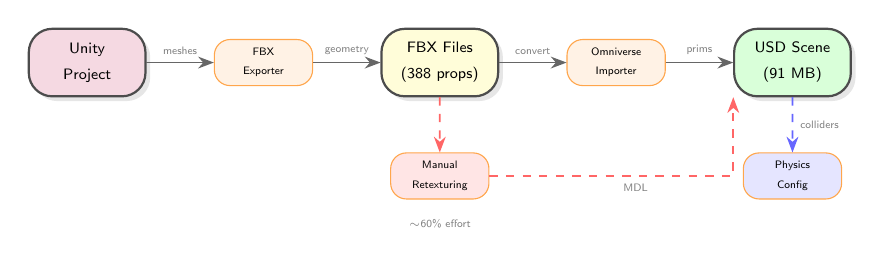
\begin{tikzpicture}[
    scale=0.78,
    transform shape,
    node distance=0.9cm,
    stage/.style={
        draw=black!70,
        rounded corners=3mm,
        minimum width=1.9cm,
        minimum height=1.1cm,
        font=\sffamily\scriptsize,
        fill=white,
        thick,
        align=center,
        drop shadow={opacity=0.2, shadow xshift=0.06cm, shadow yshift=-0.06cm}
    },
    process/.style={
        draw=orange!70,
        fill=orange!10,
        rounded corners=2mm,
        minimum width=1.6cm,
        minimum height=0.75cm,
        font=\sffamily\tiny,
        align=center
    },
    arrow/.style={->, >=Stealth, semithick, color=black!60},
    label/.style={font=\sffamily\tiny, color=black!50}
]

% Source
\node[stage, fill=purple!15] (unity) {Unity\\Project};

% Export stage
\node[process, right=1.1cm of unity] (export) {FBX\\Exporter};

% Intermediate
\node[stage, fill=yellow!15, right=1.1cm of export] (fbx) {FBX Files\\(388 props)};

% Import stage
\node[process, right=1.1cm of fbx] (import) {Omniverse\\Importer};

% Final
\node[stage, fill=green!15, right=1.1cm of import] (usd) {USD Scene\\(91 MB)};

% Arrows
\draw[arrow] (unity) -- node[above, label] {meshes} (export);
\draw[arrow] (export) -- node[above, label] {geometry} (fbx);
\draw[arrow] (fbx) -- node[above, label] {convert} (import);
\draw[arrow] (import) -- node[above, label] {prims} (usd);

% Manual processes below
\node[process, fill=red!10, below=0.9cm of fbx] (retex) {Manual\\Retexturing};
\node[process, fill=blue!10, below=0.9cm of usd] (physics) {Physics\\Config};

% Connect manual processes
\draw[arrow, dashed, red!60] (fbx.south) -- (retex.north);
\draw[arrow, dashed, red!60] (retex.east) -| node[below, label, pos=0.3] {MDL} (usd.south west);
\draw[arrow, dashed, blue!60] (usd.south) -- node[right, label] {colliders} (physics.north);

% Time annotations
\node[font=\sffamily\tiny, color=gray, below=0.2cm of retex] {$\sim$60\% effort};

\end{tikzpicture}
\caption[Unity to USD conversion pipeline]{Unity to USD conversion pipeline. The process employed FBX as an intermediate format, preserving mesh geometry and UV mappings. Manual retexturing (approximately 60\% of total effort) reconstructed materials using Omniverse MDL, followed by physics configuration for collision geometry.}
\label{fig:unity_usd_conversion}
\end{figure}

\subsubsection{Material Reconstruction and Retexturing}

The format conversion introduced significant material fidelity challenges. Unity's material system (Standard, URP, or HDRP shaders) differs fundamentally from Omniverse's MDL (Material Definition Language) materials. During FBX export, material references were preserved but texture paths became invalid, and shader parameters required manual translation to MDL equivalents.

Material reconstruction proceeded systematically across all 388 scene props. For each object, the process involved: (1) identifying original texture assets from the Unity project, (2) reimporting textures into Omniverse with correct color space settings (sRGB for albedo/diffuse, linear for normal maps and roughness), (3) creating MDL materials with appropriate parameters (base color, roughness, metallic, normal mapping), and (4) applying materials to mesh surfaces with correct UV coordinate mappings. Table \ref{tab:material_conversion} summarizes the material property mappings between Unity Standard shader and Omniverse MDL.

\begin{table}[H]
\centering
\caption{Material Property Mapping: Unity Standard Shader to Omniverse MDL}
\label{tab:material_conversion}
\footnotesize
\begin{tabular}{p{4cm}|p{4cm}|p{5cm}}
\hline
\textbf{Unity Property} & \textbf{MDL Property} & \textbf{Conversion Notes} \\
\hline
\hline
Albedo (\_MainTex) & diffuse\_color\_texture & Direct mapping, sRGB color space \\
\hline
Metallic (\_Metallic) & metallic\_constant & Value range [0,1] preserved \\
\hline
Smoothness & roughness & Inverted: roughness = 1 - smoothness \\
\hline
Normal Map (\_BumpMap) & normal\_texture & Linear color space, tangent space \\
\hline
Occlusion (\_OcclusionMap) & ao\_texture & Direct mapping, linear space \\
\hline
Emission (\_EmissionMap) & emissive\_color\_texture & Requires intensity scaling \\
\hline
\end{tabular}
\end{table}

The retexturing process accounted for approximately 60\% of total environment creation time, reflecting the labor-intensive nature of material reconstruction when crossing between incompatible material systems. However, this investment ensures visual fidelity between the digital twin and physical laboratory, enabling realistic sensor simulation (particularly for camera-based perception) and accurate lighting interactions.

\subsubsection{Physics Configuration}

Accurate physics simulation requires more than visual fidelity; collision geometry, surface properties, and contact behaviors must reflect physical reality for meaningful locomotion training. The physics configuration phase addressed three requirements: collision mesh generation, physics material assignment, and ground plane configuration.

\textbf{Collision Mesh Generation:} Visual meshes optimized for rendering often contain excessive polygon counts and non-manifold geometry unsuitable for physics simulation. For each scene object, collision approximations were generated using convex decomposition (for complex shapes) or primitive fitting (boxes, capsules, spheres for simple shapes). Isaac Sim's collision mesh generation tools automated much of this process, though manual refinement was required for objects with significant concavities or thin features.

\textbf{Physics Material Assignment:} Contact dynamics depend on surface material properties including friction coefficients and restitution (bounciness). Physics materials were assigned based on real-world surface types: concrete floors received high static friction ($\mu_s = 0.8$) and moderate dynamic friction ($\mu_d = 0.6$); metal surfaces received lower friction values; and rubber foot contacts were configured to match Unitree G1 specifications. These parameters directly influence locomotion stability and policy behavior.

\textbf{Ground Plane Configuration:} The Laboratorio Colivri features a raised floor platform where the G1 robot operates. The ground plane was set to $z = 1.2$ m elevation to match physical laboratory conditions, with robot spawn positions adjusted accordingly. This configuration ensures that trained policies exhibit correct contact dynamics and fall recovery behaviors relative to the actual deployment surface.

\begin{figure}[H]
\centering
\begin{subfigure}[b]{0.48\textwidth}
    \centering
    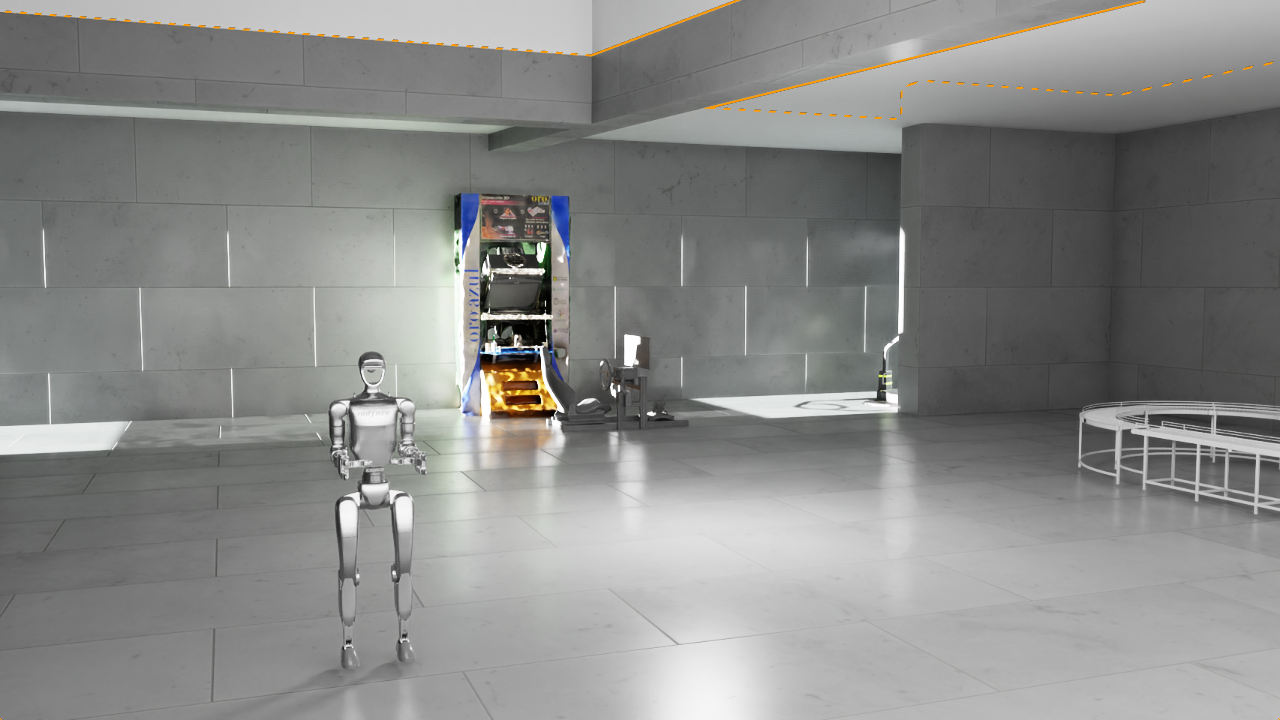
\includegraphics[width=\textwidth]{img/DigitalTwinStandard.png}
    \caption{Rendered view}
    \label{fig:colivri_rendered}
\end{subfigure}
\hfill
\begin{subfigure}[b]{0.48\textwidth}
    \centering
    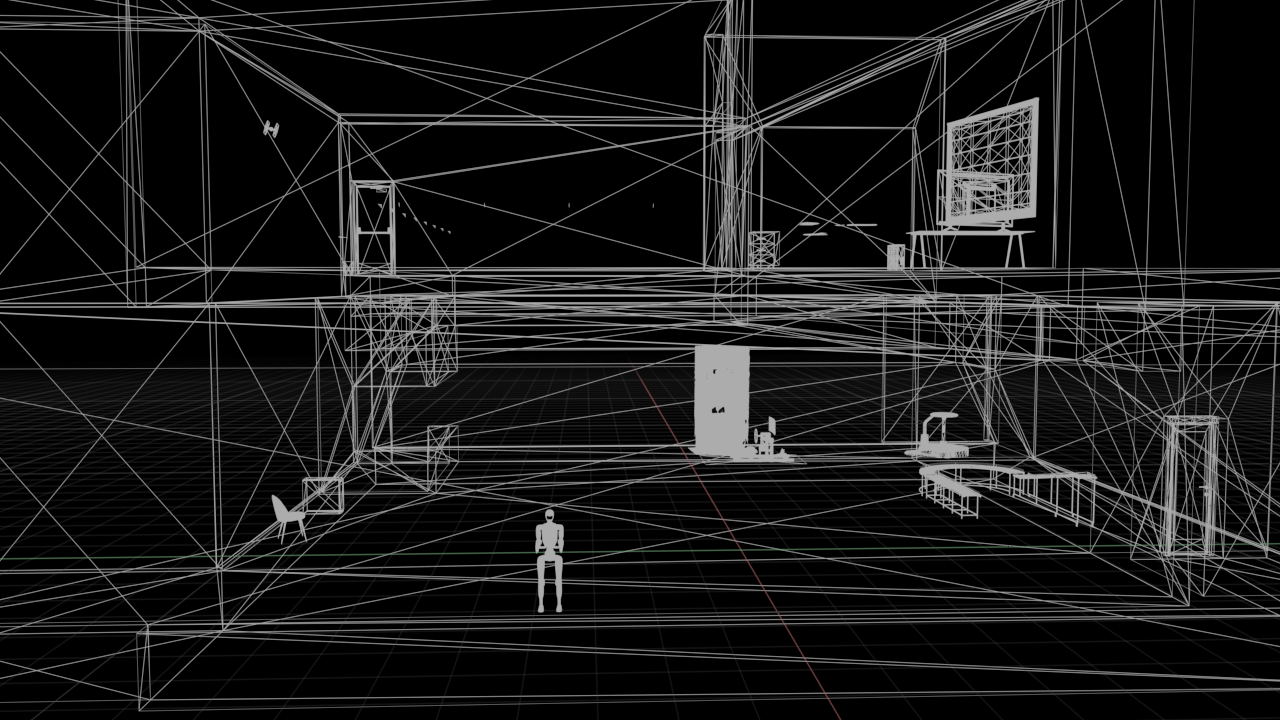
\includegraphics[width=\textwidth]{img/DigitalTwinWireframe.png}
    \caption{Wireframe view}
    \label{fig:colivri_wireframe}
\end{subfigure}
\caption[Laboratorio Colivri digital twin in Isaac Sim]{The completed Laboratorio Colivri digital twin in NVIDIA Isaac Sim with the Unitree G1 humanoid robot: (a) rendered view demonstrating visual fidelity after material reconstruction, including textured walls, floor tiles, equipment, and lighting; (b) wireframe view revealing the underlying collision geometry used for physics simulation, showing mesh structures for environment props and the robot model.}
\label{fig:colivri_environment}
\end{figure}

\subsection{Robot Integration and Isaac Lab Extension}

With the environment prepared, the second phase integrates the Unitree G1 humanoid robot into the Isaac Lab framework, establishing the simulation infrastructure for reinforcement learning. This phase involves configuring the robot model, creating an Isaac Lab extension for project-specific customizations, and registering gymnasium-compatible training environments.

\subsubsection{Unitree G1 Robot Configuration}

The Unitree G1 humanoid robot provides 29 actuated degrees of freedom distributed across lower body (12 DOF: hip, knee, ankle), upper body (14 DOF: shoulder, elbow, wrist), and torso (3 DOF: waist). Figure \ref{fig:g1_component_overview} illustrates the robot's hardware architecture, showing the distribution of joint motors, sensors, and structural components. Table \ref{tab:g1_dof} details the joint distribution and range limits.

\begin{figure}[H]
\centering
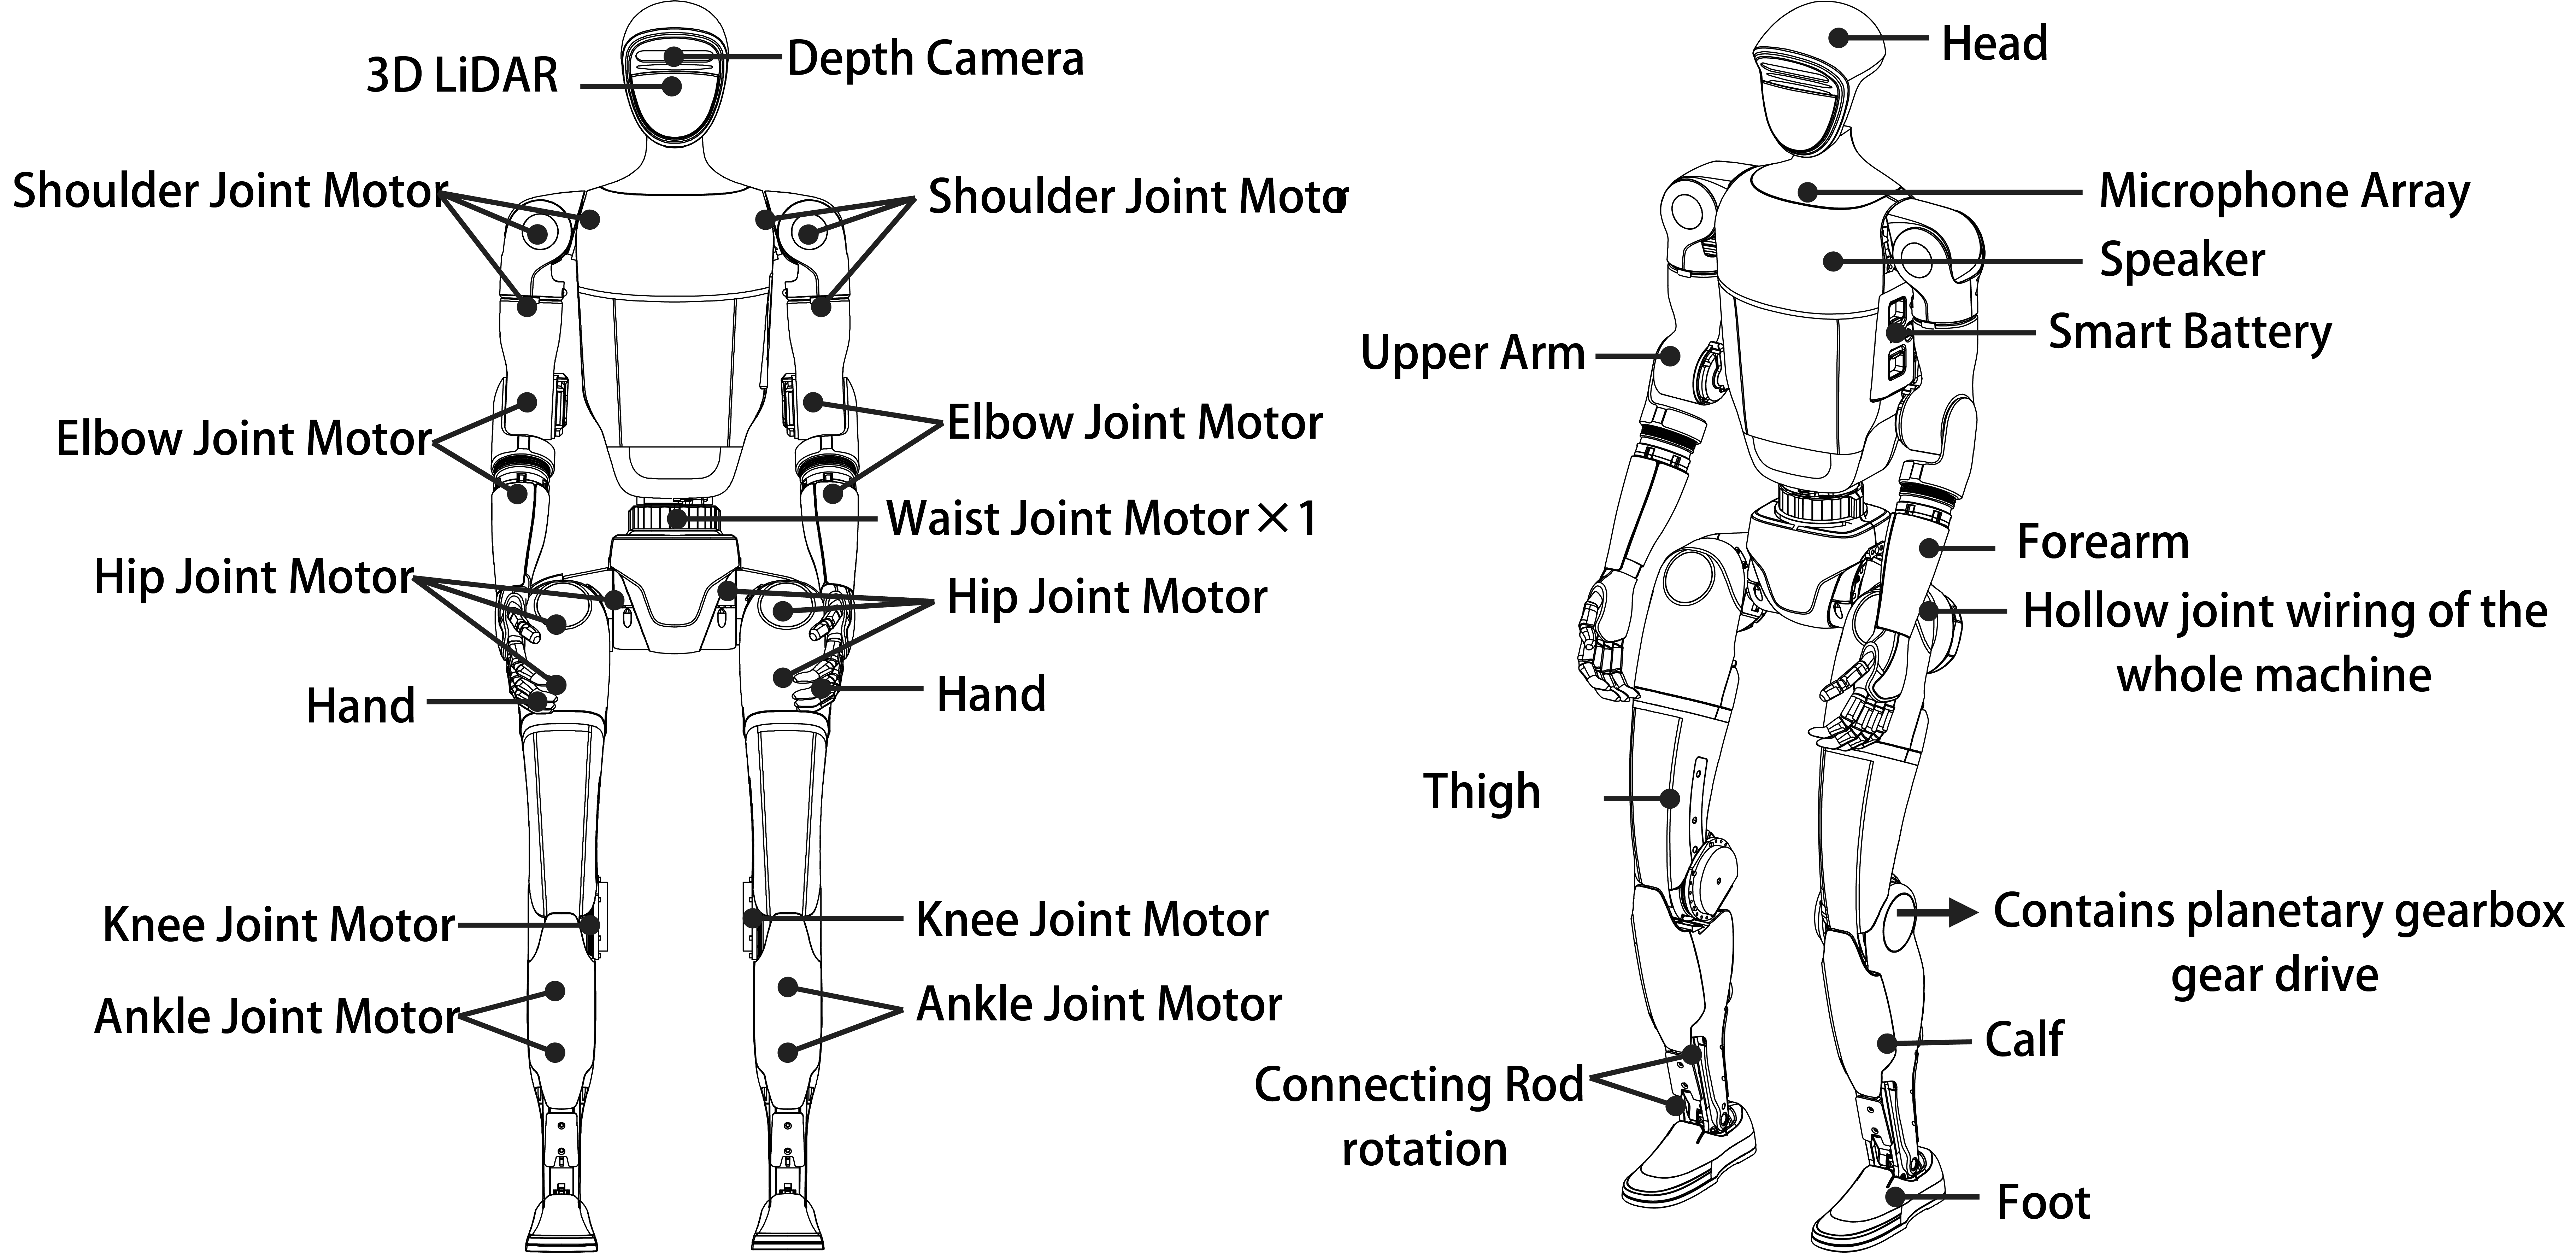
\includegraphics[width=0.85\textwidth]{img/g1_component_overview.png}
\caption[Unitree G1 hardware component overview]{Unitree G1 humanoid robot hardware component overview showing the distribution of joint motors across the kinematic chain (left: front view, right: side view). The platform integrates 3D LiDAR and depth camera sensors in the head unit, with actuators distributed across shoulder, elbow, hip, knee, and ankle joints. Adapted from \textcite{quadrupedde2024g1}.}
\label{fig:g1_component_overview}
\end{figure}

\begin{table}[H]
\centering
\caption{Unitree G1 Joint Configuration (29 DOF)}
\label{tab:g1_dof}
\footnotesize
\begin{tabular}{l|c|c|l}
\hline
\textbf{Body Part} & \textbf{Joints per Side} & \textbf{Total DOF} & \textbf{Joint Types} \\
\hline
\hline
Hip & 3 & 6 & Roll, pitch, yaw \\
\hline
Knee & 1 & 2 & Pitch \\
\hline
Ankle & 2 & 4 & Pitch, roll \\
\hline
Waist & 3 (central) & 3 & Roll, pitch, yaw \\
\hline
Shoulder & 3 & 6 & Roll, pitch, yaw \\
\hline
Elbow & 1 & 2 & Pitch \\
\hline
Wrist & 1 & 2 & Roll \\
\hline
Gripper & 2 & 4 & Finger joints (fixed in locomotion) \\
\hline
\textbf{Total Actuated} & --- & \textbf{29} & --- \\
\hline
\end{tabular}
\end{table}

The robot configuration inherits from Isaac Lab's proven \texttt{G1FlatEnvCfg} base class, which provides validated motor parameters, joint limits, and default poses established through prior sim-to-real transfer work \parencite{gu2024humanoidgym}. This inheritance strategy leverages existing validation while enabling project-specific customizations for goal-directed navigation.

\subsubsection{Isaac Lab Extension Architecture}

The project implements a standalone Isaac Lab extension (\texttt{digital\_twin\_colivri\_g1}) following NVIDIA's recommended extension pattern. This architecture enables custom environment definitions, reward functions, and command generators while maintaining compatibility with Isaac Lab's core infrastructure. Figure \ref{fig:extension_architecture} illustrates the extension structure, and Table \ref{tab:extension_components} describes the key components.

\begin{figure}[H]
\centering
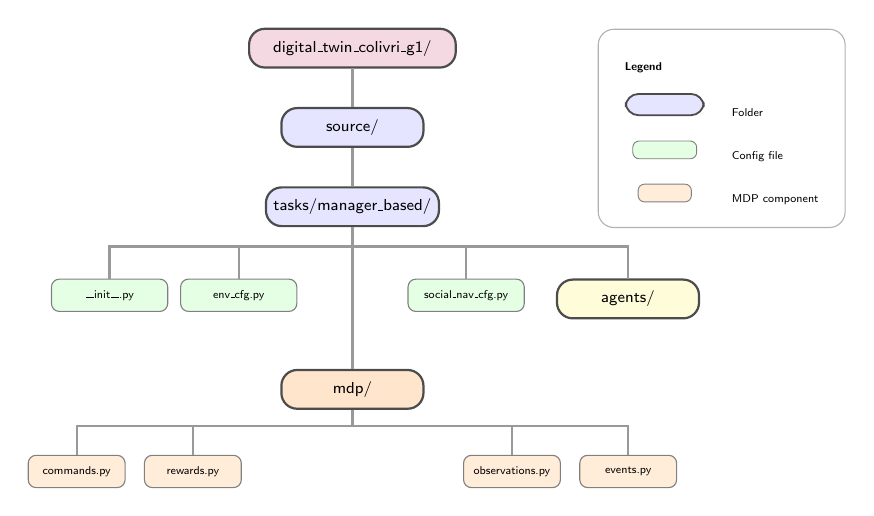
\begin{tikzpicture}[
    scale=0.82,
    transform shape,
    node distance=0.4cm,
    folder/.style={
        draw=black!70,
        rounded corners=2mm,
        minimum width=2.2cm,
        minimum height=0.6cm,
        font=\sffamily\scriptsize,
        fill=blue!10,
        thick,
        align=center
    },
    file/.style={
        draw=black!50,
        rounded corners=1mm,
        minimum width=1.8cm,
        minimum height=0.5cm,
        font=\sffamily\tiny,
        fill=green!10,
        align=center
    },
    mdpfile/.style={
        draw=black!50,
        rounded corners=1mm,
        minimum width=1.5cm,
        minimum height=0.5cm,
        font=\sffamily\tiny,
        fill=orange!15,
        align=center
    },
    arrow/.style={-, thick, color=black!40}
]

% Root
\node[folder, fill=purple!15, minimum width=3.2cm] (root) {digital\_twin\_colivri\_g1/};

% Source level
\node[folder, below=0.6cm of root] (source) {source/};
\draw[arrow] (root.south) -- (source.north);

% Tasks level
\node[folder, below=0.6cm of source] (tasks) {tasks/manager\_based/};
\draw[arrow] (source.south) -- (tasks.north);

% Main files and folders - horizontal spread
\node[file, below left=0.8cm and 1.5cm of tasks] (init) {\_\_init\_\_.py};
\node[file, below left=0.8cm and -0.5cm of tasks] (envcfg) {env\_cfg.py};
\node[file, below right=0.8cm and -0.5cm of tasks] (socialcfg) {social\_nav\_cfg.py};
\node[folder, fill=yellow!15, below right=0.8cm and 1.8cm of tasks] (agents) {agents/};
\node[folder, fill=orange!20, below=2.2cm of tasks] (mdp) {mdp/};

% Connect to tasks
\draw[arrow] (tasks.south) -- ++(0,-0.3) -| (init.north);
\draw[arrow] (tasks.south) -- ++(0,-0.3) -| (envcfg.north);
\draw[arrow] (tasks.south) -- ++(0,-0.3) -| (socialcfg.north);
\draw[arrow] (tasks.south) -- ++(0,-0.3) -| (agents.north);
\draw[arrow] (tasks.south) -- (mdp.north);

% MDP components - spread out more
\node[mdpfile, below left=0.7cm and 2.4cm of mdp] (commands) {commands.py};
\node[mdpfile, below left=0.7cm and 0.6cm of mdp] (rewards) {rewards.py};
\node[mdpfile, below right=0.7cm and 0.6cm of mdp] (obs) {observations.py};
\node[mdpfile, below right=0.7cm and 2.4cm of mdp] (events) {events.py};

% Connect MDP
\draw[arrow] (mdp.south) -- ++(0,-0.25) -| (commands.north);
\draw[arrow] (mdp.south) -- ++(0,-0.25) -| (rewards.north);
\draw[arrow] (mdp.south) -- ++(0,-0.25) -| (obs.north);
\draw[arrow] (mdp.south) -- ++(0,-0.25) -| (events.north);

% Legend - positioned at top right
\node[draw=black!30, rounded corners=2mm, fill=white, inner sep=0.2cm, anchor=north west] at (3.8,0.3) {
    \begin{tabular}{cl}
    \multicolumn{2}{l}{\textbf{\sffamily\tiny Legend}} \\[2pt]
    \tikz\node[folder, scale=0.55] {}; & \sffamily\tiny Folder \\[1pt]
    \tikz\node[file, scale=0.55] {}; & \sffamily\tiny Config file \\[1pt]
    \tikz\node[mdpfile, scale=0.55] {}; & \sffamily\tiny MDP component
    \end{tabular}
};

\end{tikzpicture}
\caption[Isaac Lab extension architecture]{Isaac Lab extension architecture for the digital twin project. The extension follows NVIDIA's recommended pattern with environment configurations at the task level and custom MDP components (commands, rewards, observations, events) in a dedicated subdirectory.}
\label{fig:extension_architecture}
\end{figure}

\begin{table}[H]
\centering
\caption{Extension Component Descriptions}
\label{tab:extension_components}
\footnotesize
\begin{tabular}{l|l|p{7cm}}
\hline
\textbf{Component} & \textbf{Type} & \textbf{Description} \\
\hline
\hline
\texttt{\_\_init\_\_.py} & Config & Gymnasium task registration and entry points \\
\hline
\texttt{env\_cfg.py} & Config & Base environment configuration (512 envs, rewards, commands) \\
\hline
\texttt{social\_nav\_cfg.py} & Config & Social navigation variant with LiDAR and obstacles \\
\hline
\texttt{agents/} & Folder & PPO hyperparameter configurations (RSL-RL, SKRL) \\
\hline
\texttt{commands.py} & MDP & Goal position and velocity command generators (570 LOC) \\
\hline
\texttt{rewards.py} & MDP & Navigation reward functions (409 LOC) \\
\hline
\texttt{observations.py} & MDP & State observations including LiDAR sectors (91 LOC) \\
\hline
\texttt{events.py} & MDP & Environment events and obstacle spawning (162 LOC) \\
\hline
\end{tabular}
\end{table}

The extension registers four gymnasium-compatible tasks, summarized in Table \ref{tab:registered_tasks}:

\begin{table}[H]
\centering
\caption{Registered Gymnasium Tasks}
\label{tab:registered_tasks}
\footnotesize
\begin{tabular}{l|c|p{6.5cm}}
\hline
\textbf{Task ID} & \textbf{Envs} & \textbf{Description} \\
\hline
\hline
\texttt{Isaac-Colivri-G1-v0} & 512 & Training with goal-directed navigation and domain randomization \\
\hline
\texttt{Isaac-Colivri-G1-Play-v0} & 10 & Evaluation with disabled randomization for visualization \\
\hline
\texttt{Isaac-Colivri-G1-SocialNav-v0} & 128 & Social navigation training with LiDAR and obstacle avoidance \\
\hline
\texttt{Isaac-Colivri-G1-SocialNav-Play-v0} & 4 & Social navigation evaluation with sensor visualization \\
\hline
\end{tabular}
\end{table}

\subsection{Custom RL Task Design for Goal-Directed Navigation}

The third phase implements the core contribution of this work: a custom reinforcement learning task that enables point-to-point navigation through direct low-level joint control. Unlike hierarchical approaches that require separate trajectory planners and joint controllers, this task trains a single policy network to map goal positions and robot state directly to 29-DOF joint commands. The implementation comprises three interconnected components: goal command generation, goal-directed velocity commands, and custom reward functions.

\subsubsection{Goal Command Generation}

Navigation tasks require the robot to reach specified goal positions. The \texttt{SimpleGoalCommand} class generates goal positions and resamples goals throughout training episodes. Key design decisions address distribution shift and behavioral stability:

\textbf{Forward-Biased Goal Sampling:} Random uniform goal sampling often places targets behind the robot, requiring 180-degree rotations before forward progress can be made. This creates training instability and encourages stationary pivoting rather than efficient locomotion. The implementation biases goal sampling toward the robot's forward direction: at episode initialization, 80\% of goals spawn within a 30-degree forward cone, with the remaining 20\% in the forward hemisphere ($\pm$90 degrees). After reaching a goal, subsequent goals use 65\% forward bias to maintain locomotion momentum while introducing navigational variety.

\textbf{Reach-Based Resampling:} Traditional approaches resample goals at fixed time intervals regardless of task progress. This work employs reach-based resampling: new goals generate only when the robot achieves proximity to the current target (distance $< 0.3$ m). This approach ensures the policy receives consistent training signal for goal approach behaviors rather than arbitrary goal transitions.

\textbf{Smooth Goal Transitions:} Instantaneous goal changes can destabilize locomotion as velocity commands shift abruptly. The implementation interpolates between consecutive goals over 1.5 seconds, providing smooth command transitions that maintain balance during navigation.

\begin{figure}[H]
\centering
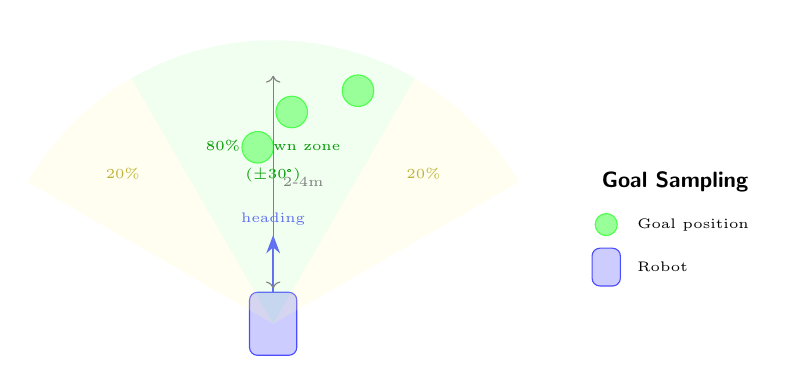
\begin{tikzpicture}[
    scale=0.9,
    robot/.style={draw=blue!70, fill=blue!20, minimum width=0.6cm, minimum height=0.8cm, rounded corners=1mm},
    goal/.style={draw=green!70, fill=green!40, circle, minimum size=0.4cm},
    zone/.style={draw=none, fill opacity=0.2},
    arrow/.style={->, >=Stealth, thick}
]

% Robot
\node[robot] (robot) at (0,0) {};
\draw[arrow, blue!70] (robot.north) -- ++(0,0.8) node[above, font=\tiny] {heading};

% Forward cone (80% at spawn)
\fill[zone, fill=green!30] (0,0) -- (60:4) arc (60:120:4) -- cycle;
\node[font=\tiny, green!60!black] at (90:2.5) {80\% spawn zone};
\node[font=\tiny, green!60!black] at (90:2.1) {($\pm$30°)};

% Forward hemisphere (20% at spawn, 65% after reaching)
\fill[zone, fill=yellow!30] (0,0) -- (30:4) arc (30:60:4) -- cycle;
\fill[zone, fill=yellow!30] (0,0) -- (120:4) arc (120:150:4) -- cycle;
\node[font=\tiny, yellow!70!black] at (45:3) {20\%};
\node[font=\tiny, yellow!70!black] at (135:3) {20\%};

% Goals
\node[goal] at (85:3) {};
\node[goal] at (95:2.5) {};
\node[goal] at (70:3.5) {};

% Distance annotations
\draw[<->, thin, gray] (0,0.5) -- node[right, font=\tiny] {2-4m} (90:3.5);

% Legend
\node[font=\sffamily\footnotesize, anchor=west] at (4.5,2) {\textbf{Goal Sampling}};
\node[goal, scale=0.7] at (4.7,1.4) {};
\node[font=\tiny, anchor=west] at (5,1.4) {Goal position};
\node[robot, scale=0.6] at (4.7,0.8) {};
\node[font=\tiny, anchor=west] at (5,0.8) {Robot};

\end{tikzpicture}
\caption[Forward-biased goal sampling distribution]{Forward-biased goal sampling distribution. At episode initialization, 80\% of goals spawn in a narrow forward cone ($\pm$30°) with 20\% in the extended forward hemisphere. This bias encourages forward locomotion development while ensuring navigational coverage. Goals spawn at 2-4 meter distances from the robot.}
\label{fig:goal_sampling}
\end{figure}

\subsubsection{Goal-Directed Velocity Commands}

While goal positions specify navigation targets, the locomotion policy operates on velocity commands (linear velocity $v_x$, $v_y$ and angular velocity $\omega_z$). The \texttt{GoalDirectedVelocityCommand} class transforms goal positions into velocity commands that guide the robot toward targets. This transformation incorporates three scaling mechanisms:

\textbf{Distance-Based Speed Scaling:} Velocity magnitude scales with distance to goal. When far from the target ($>3$ m), full forward velocity is commanded. As distance decreases, velocity reduces proportionally to enable precise terminal positioning:
\begin{equation}
v_{scale} = v_{min} + (1 - v_{min}) \cdot \min\left(1, \frac{d_{goal}}{d_{threshold}}\right)
\end{equation}
where $v_{min} = 0.2$ (20\% minimum velocity), $d_{goal}$ is current distance to goal, and $d_{threshold} = 3.0$ m.

\textbf{Heading-Aware Modulation:} Forward velocity further scales based on angular alignment with the goal. When facing the target (heading error $< 15^\circ
$), full scaled velocity applies. When perpendicular or facing away, forward velocity reduces to prioritize rotational correction:
\begin{equation}
v_{heading} = 0.4 + 0.6 \cdot \cos(\theta_{error})
\end{equation}
where $\theta_{error}$ is the angle between robot's heading and the goal direction.

\textbf{No Backwards Motion:} The velocity command enforces $v_x \geq 0$, preventing backwards locomotion that often indicates policy confusion or local minima. The robot must rotate to face goals rather than walking backwards, promoting stable forward gait development.

\textbf{Proportional Angular Control:} Angular velocity commands apply proportional control toward the goal direction with gain $K_\omega = 5.0$:
\begin{equation}
\omega_z = K_\omega \cdot \theta_{error}
\end{equation}
clamped to actuator limits ($\pm 1.0$ rad/s).

\subsubsection{Custom Reward Functions}

The reward function guides policy learning toward desired navigation behaviors while maintaining locomotion stability. The design balances multiple objectives through weighted reward terms, inheriting proven velocity-tracking rewards from the G1 base configuration while adding navigation-specific terms.

\textbf{Dual Exponential Goal Distance Rewards:} Two exponential terms provide multi-scale goal approach incentives:
\begin{align}
r_{coarse} &= 0.3 \cdot \exp\left(-\frac{d_{goal}^2}{\sigma_{coarse}^2}\right), \quad \sigma_{coarse} = 5.0 \\
r_{fine} &= 0.2 \cdot \exp\left(-\frac{d_{goal}^2}{\sigma_{fine}^2}\right), \quad \sigma_{fine} = 3.0
\end{align}
The coarse term ($\sigma = 5.0$) provides gradient across the full navigation range, while the fine term ($\sigma = 3.0$) sharpens reward near the goal for precise positioning.

\textbf{Heading Alignment Reward:} Encourages the robot to face toward the goal:
\begin{equation}
r_{heading} = 0.3 \cdot \exp\left(-\frac{\theta_{error}^2}{\sigma_{heading}^2}\right), \quad \sigma_{heading} = 0.5
\end{equation}

\textbf{Backwards Velocity Penalty:} Discourages backwards motion that indicates policy confusion:
\begin{equation}
r_{backwards} = -0.5 \cdot \mathbb{1}[v_x < -0.1]
\end{equation}

\textbf{Reward Balance:} The velocity tracking reward (weight 1.0) ensures stable locomotion, while navigation rewards (combined weight 0.8) provide directional guidance. This ratio emerged from empirical tuning---higher navigation weights destabilized learned gaits, while lower weights slowed goal convergence. The complete reward specification, including mathematical definitions is provided in Table \ref{tab:reward_specification} (Section 4.1.4).

The 125-dimensional observation space and domain randomization parameters are formally specified in Section 4.1 (Tables \ref{tab:state_space} and \ref{tab:domain_randomization}).

\subsection{Policy Training}

The fourth phase applies Proximal Policy Optimization (PPO) to train locomotion policies using the task configuration from Phase 3. Training leverages Isaac Lab's GPU-accelerated parallel simulation to achieve sample-efficient learning on a single workstation.

\subsubsection{Training Configuration}

Training employs 512 parallel environment instances, enabling collection of 512 state-action-reward tuples per simulation step. This parallelism accelerates training by approximately 100$\times$ compared to sequential simulation, completing policy training in 3-4 hours on an NVIDIA RTX 4080 GPU.

The PPO configuration inherits from \texttt{G1FlatPPORunnerCfg}, which provides validated hyperparameters from prior sim-to-real transfer work:

\begin{table}[H]
\centering
\caption{PPO Training Hyperparameters}
\label{tab:ppo_config}
\footnotesize
\begin{tabular}{l|c|l}
\hline
\textbf{Parameter} & \textbf{Value} & \textbf{Description} \\
\hline
\hline
Learning rate & $1 \times 10^{-3}$ & Adam optimizer \\
\hline
Discount factor ($\gamma$) & 0.99 & Future reward weighting \\
\hline
GAE lambda ($\lambda$) & 0.95 & Advantage estimation \\
\hline
Clip range ($\epsilon$) & 0.2 & Policy update constraint \\
\hline
Entropy coefficient & 0.01 & Exploration bonus \\
\hline
Value function coefficient & 0.5 & Critic loss weighting \\
\hline
Mini-batch size & 4096 & Samples per gradient update \\
\hline
Number of epochs & 5 & Passes over collected data \\
\hline
Network architecture & [512, 256, 128] & MLP hidden layers \\
\hline
Activation function & ELU & Nonlinearity \\
\hline
\end{tabular}
\end{table}

Figure \ref{fig:ppo_architecture} illustrates the actor-critic network architecture used in PPO training.

\begin{figure}[H]
\centering
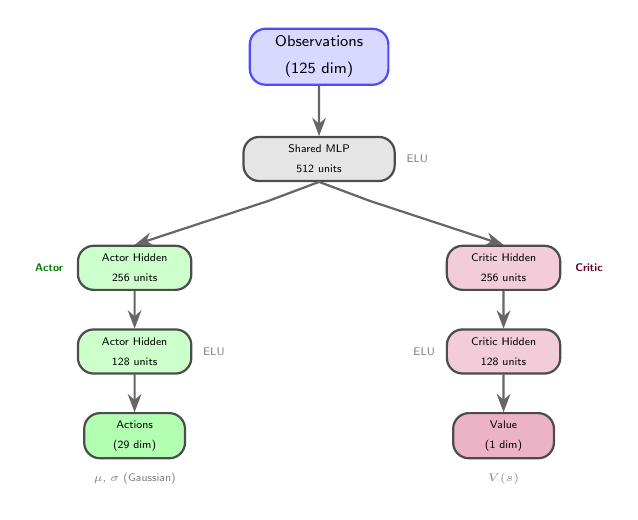
\begin{tikzpicture}[
    scale=0.8,
    transform shape,
    node distance=0.6cm,
    layer/.style={
        draw=black!70,
        rounded corners=2mm,
        minimum width=1.8cm,
        minimum height=0.7cm,
        font=\sffamily\tiny,
        thick,
        align=center
    },
    input/.style={
        draw=blue!70,
        fill=blue!15,
        rounded corners=2mm,
        minimum width=2.2cm,
        minimum height=0.8cm,
        font=\sffamily\scriptsize,
        thick,
        align=center
    },
    output/.style={
        draw=black!70,
        rounded corners=2mm,
        minimum width=1.6cm,
        minimum height=0.7cm,
        font=\sffamily\tiny,
        thick,
        align=center
    },
    arrow/.style={->, >=Stealth, thick, color=black!60}
]

% Input
\node[input] (obs) {Observations\\(125 dim)};

% Shared layers
\node[layer, fill=gray!20, below=0.8cm of obs, minimum width=2.4cm] (shared) {Shared MLP\\512 units};

% Split into actor and critic
\node[layer, fill=green!20, below left=1cm and 0.8cm of shared] (actor1) {Actor Hidden\\256 units};
\node[layer, fill=purple!20, below right=1cm and 0.8cm of shared] (critic1) {Critic Hidden\\256 units};

\node[layer, fill=green!20, below=0.6cm of actor1] (actor2) {Actor Hidden\\128 units};
\node[layer, fill=purple!20, below=0.6cm of critic1] (critic2) {Critic Hidden\\128 units};

% Outputs
\node[output, fill=green!30, below=0.6cm of actor2] (actions) {Actions\\(29 dim)};
\node[output, fill=purple!30, below=0.6cm of critic2] (value) {Value\\(1 dim)};

% Labels
\node[font=\sffamily\tiny\bfseries, green!50!black, left=0.1cm of actor1] {Actor};
\node[font=\sffamily\tiny\bfseries, purple!50!black, right=0.1cm of critic1] {Critic};

% Arrows
\draw[arrow] (obs) -- (shared);
\draw[arrow] (shared.south) -- ++(-0.8,-0.3) -- (actor1.north);
\draw[arrow] (shared.south) -- ++(0.8,-0.3) -- (critic1.north);
\draw[arrow] (actor1) -- (actor2);
\draw[arrow] (critic1) -- (critic2);
\draw[arrow] (actor2) -- (actions);
\draw[arrow] (critic2) -- (value);

% Activation annotations
\node[font=\sffamily\tiny, color=gray, right=0.05cm of shared.east] {ELU};
\node[font=\sffamily\tiny, color=gray, right=0.05cm of actor2.east] {ELU};
\node[font=\sffamily\tiny, color=gray, left=0.05cm of critic2.west] {ELU};

% Output annotations
\node[font=\sffamily\tiny, color=gray, below=0.1cm of actions] {$\mu$, $\sigma$ (Gaussian)};
\node[font=\sffamily\tiny, color=gray, below=0.1cm of value] {$V(s)$};

\end{tikzpicture}
\caption[PPO actor-critic network architecture]{PPO actor-critic network architecture. The policy receives 125-dimensional observations and outputs 29-dimensional joint position targets through the actor branch, while the critic branch estimates state values for advantage computation. Both branches share initial feature extraction before specializing.}
\label{fig:ppo_architecture}
\end{figure}

\textbf{Design Rationale.} Several configuration choices merit justification:

\textit{Parallel environments (512):} The number of parallel environments balances GPU memory utilization against sample diversity. With 512 environments, each PPO iteration collects 512$\times$512 = 262,144 samples, providing sufficient batch diversity for stable gradient estimation. Increasing to 1024+ environments exceeds available GPU memory (12GB on RTX 4080 Super) when combined with the 29-DOF robot model and ray-casting overhead. Decreasing the number of environments below 256 slows training disproportionately, as GPU utilization becomes suboptimal.

\textit{Network architecture [512, 256, 128]:} The three-layer MLP architecture follows HumanoidGym's validated configuration, which achieved successful sim-to-real transfer on the same robot platform. The decreasing layer widths (512$\rightarrow$256$\rightarrow$128) progressively compress the 125-dimensional observation into a compact representation suitable for the 29-dimensional action output. Deeper or wider networks were not explored, as the inherited architecture proved sufficient for the task; network architecture ablations remain for future work.

\textit{Learning rate ($10^{-3}$) with adaptive schedule:} The initial learning rate enables rapid early progress, while the adaptive schedule (based on KL divergence monitoring) reduces the rate as training progresses, preventing oscillation near convergence. This schedule is implemented in RSL-RL and activates automatically when policy updates become too aggressive.

\textit{Entropy coefficient (0.01):} The entropy bonus encourages exploration by penalizing deterministic policies. The value 0.01 maintains moderate exploration throughout training; higher values (0.05-0.1) caused unstable locomotion in preliminary experiments, while lower values (0.001) led to premature convergence to suboptimal gaits.

\subsubsection{Domain Randomization}

To promote sim-to-real transfer robustness, training applies domain randomization over physical parameters:

\begin{itemize}
    \item \textbf{Mass variation:} $\pm$15\% randomization on link masses
    \item \textbf{Friction coefficients:} Ground friction uniformly sampled from [0.5, 1.2]
    \item \textbf{Joint damping:} $\pm$20\% variation on damping coefficients
    \item \textbf{Motor strength:} $\pm$10\% scaling on torque limits
    \item \textbf{Observation noise:} Gaussian noise on joint positions ($\sigma = 0.01$ rad) and velocities ($\sigma = 0.1$ rad/s)
    \item \textbf{Action delay:} Random 1-3 step delays on command execution
\end{itemize}

This randomization ensures policies experience diverse physical conditions during training, encouraging robust behaviors that generalize across parameter variations encountered during physical deployment.

\textbf{Design Rationale for Randomization Ranges.} The specific randomization ranges derive from common practice in legged robotics rather than measured hardware variation on the physical Unitree G1:

\textit{Mass variation ($\pm$15\%):} This range accounts for manufacturing tolerances (typically $\pm$5\%), payload attachment (up to 10\% body mass), and potential future modifications. The range follows recommendations from \textcite{hwangbo2019learning} for quadruped locomotion.

\textit{Friction coefficients ([0.5, 1.2]):} The range spans typical indoor surfaces (polished concrete $\mu \approx 0.5$, rubber flooring $\mu \approx 1.0$+). The upper bound exceeds typical measured values to provide a safety margin for sticky surfaces.

\textit{Joint damping ($\pm$20\%) and motor strength ($\pm$10\%):} These ranges approximate expected actuator variation due to temperature, wear, and manufacturing tolerances. Actuator characterization data for Unitree G1 were not available; ranges follow conservative estimates from similar platforms.

\textit{Action delay (1-3 steps):} At 50Hz control frequency, this corresponds to 20-60ms latency, covering expected communication and processing delays in the ROS2-based deployment pipeline. The sim2sim infrastructure introduces similar latencies, making this randomization particularly relevant.

Ideally, these ranges would derive from systematic hardware measurements. The current values represent conservative approximations that prioritize robustness over optimality; overly narrow ranges risk brittle policies that fail on real hardware, while overly wide ranges may unnecessarily constrain achievable performance.

\subsubsection{Training Procedure}

Training proceeds for approximately 2000-3000 iterations, with each iteration collecting 512 environment steps (262,144 total samples) and then performing 5 PPO update epochs. Checkpoints are saved every 100 iterations, enabling recovery from training failures and comparison across training stages.

\begin{figure}[H]
\centering
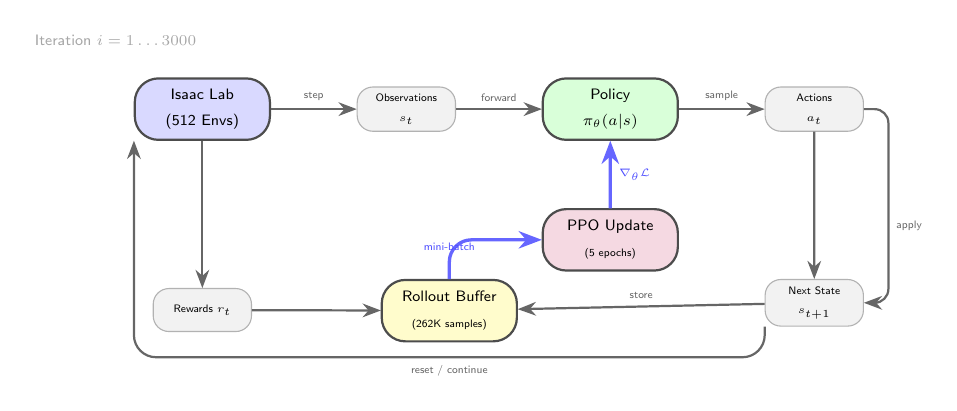
\begin{tikzpicture}[
    scale=0.78,
    transform shape,
    node distance=0.8cm,
    component/.style={
        draw=black!70,
        rounded corners=3mm,
        minimum width=2.2cm,
        minimum height=1cm,
        font=\sffamily\scriptsize,
        thick,
        align=center
    },
    data/.style={
        draw=gray!60,
        fill=gray!10,
        rounded corners=2mm,
        minimum width=1.6cm,
        minimum height=0.7cm,
        font=\sffamily\tiny,
        align=center
    },
    arrow/.style={->, >=Stealth, thick, color=black!60},
    bluearrow/.style={->, >=Stealth, very thick, color=blue!60}
]

% Top row - main forward pass
\node[component, fill=blue!15] (env) {Isaac Lab\\(512 Envs)};
\node[data, right=1.4cm of env] (obs) {Observations\\$s_t$};
\node[component, fill=green!15, right=1.4cm of obs] (policy) {Policy\\$\pi_\theta(a|s)$};
\node[data, right=1.4cm of policy] (actions) {Actions\\$a_t$};

% Middle row - PPO Update (raised to avoid overlapping arrows)
\node[component, fill=purple!15, below=1.1cm of policy] (update) {PPO Update\\{\tiny (5 epochs)}};

% Bottom row - data collection (buffer shifted right for better spacing)
\node[data, below=2.4cm of env] (rewards) {Rewards $r_t$};
\node[component, fill=yellow!20, below=2.4cm of obs, xshift=0.7cm] (buffer) {Rollout Buffer\\{\tiny (262K samples)}};
\node[data, below=2.4cm of actions] (next) {Next State\\$s_{t+1}$};

% Forward arrows (top)
\draw[arrow] (env) -- node[above, font=\sffamily\tiny] {step} (obs);
\draw[arrow] (obs) -- node[above, font=\sffamily\tiny] {forward} (policy);
\draw[arrow] (policy) -- node[above, font=\sffamily\tiny] {sample} (actions);

% Down arrows from top to bottom
\draw[arrow] (env.south) -- (rewards.north);
\draw[arrow] (actions.south) -- (next.north);

% Bottom flow: rewards and next state feed into buffer (straight arrows)
\draw[arrow] (rewards) -- (buffer);
\draw[arrow] (next) -- node[above, font=\sffamily\tiny] {store} (buffer);

% Mini-batch arrow: from buffer top, curves to PPO update left side
\draw[bluearrow, rounded corners=8pt] (buffer.north) |- node[above, font=\sffamily\tiny, color=blue!70, pos=0.25] {mini-batch} (update.west);

% Gradient update arrow: PPO update up to policy
\draw[bluearrow] (update.north) -- node[right, font=\sffamily\tiny, color=blue!70] {$\nabla_\theta \mathcal{L}$} (policy.south);

% Loop back arrow (starts from next.south west to avoid overlap)
\draw[arrow, rounded corners=8pt] (next.south west) -- ++(0,-0.5) -| node[below, font=\sffamily\tiny, pos=0.25] {reset / continue} (env.south west);

% Apply arrow on right side
\draw[arrow, rounded corners=5pt] (actions.east) -- ++(0.4,0) |- node[right, font=\sffamily\tiny, pos=0.3] {apply} (next.east);

% Title annotation
\node[font=\sffamily\scriptsize, color=gray!70, anchor=south] at ($(env.north west) + (-0.3, 0.4)$) {Iteration $i = 1 \ldots 3000$};

\end{tikzpicture}
\caption[PPO training procedure]{PPO training procedure. Each iteration collects 512 parallel environment steps and stores state-action-reward tuples in a rollout buffer. After accumulating 262,144 samples, PPO performs 5 update epochs on mini-batches, computing policy gradients $\nabla_\theta \mathcal{L}$ using the clipped surrogate objective. The loop continues for 2000-3000 iterations until convergence.}
\label{fig:training_procedure}
\end{figure}

\subsection{Simulation-to-Simulation ROS 2 Validation}

The fifth phase implements the communication-realistic validation framework that distinguishes this work from direct sim-to-real approaches. Trained policies are evaluated in a second simulation environment that employs authentic ROS 2 Humble communication protocols, validating performance under realistic message passing constraints before physical deployment.

\subsubsection{Validation Architecture}

The sim2sim validation environment replicates communication patterns present in physical Unitree G1 deployments. Rather than invoking the policy through direct Python function calls (as during training), state observations and control commands flow through ROS 2 topics with realistic serialization, transport, and timing characteristics.

\begin{figure}[H]
\centering
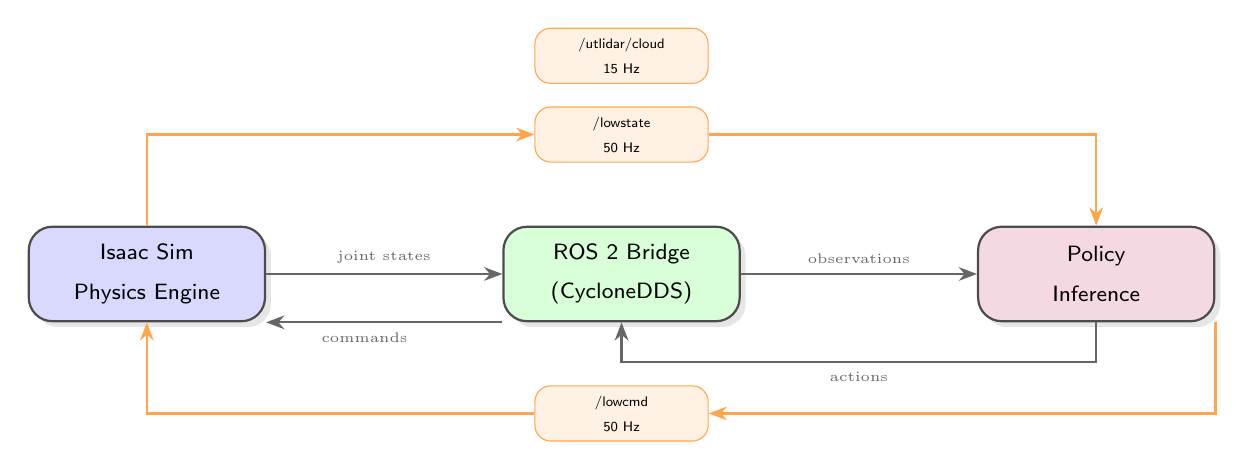
\begin{tikzpicture}[
    node distance=1cm and 2cm,
    component/.style={
        draw=black!70,
        rounded corners=3mm,
        minimum width=3cm,
        minimum height=1.2cm,
        font=\sffamily\footnotesize,
        fill=white,
        thick,
        align=center,
        drop shadow={opacity=0.2}
    },
    topic/.style={
        draw=orange!70,
        fill=orange!10,
        rounded corners=2mm,
        minimum width=2.2cm,
        minimum height=0.7cm,
        font=\sffamily\tiny,
        align=center
    },
    arrow/.style={->, >=Stealth, thick, color=black!60}
]

% Isaac Sim
\node[component, fill=blue!15] (sim) {Isaac Sim\\Physics Engine};

% ROS2 Bridge
\node[component, fill=green!15, right=3cm of sim] (bridge) {ROS 2 Bridge\\(CycloneDDS)};

% Policy Node
\node[component, fill=purple!15, right=3cm of bridge] (policy) {Policy\\Inference};

% Topics
\node[topic, above=0.8cm of bridge] (lowstate) {/lowstate\\50 Hz};
\node[topic, below=0.8cm of bridge] (lowcmd) {/lowcmd\\50 Hz};
\node[topic, above=1.8cm of bridge] (lidar) {/utlidar/cloud\\15 Hz};

% Arrows
\draw[arrow] (sim.east) -- node[above, font=\tiny] {joint states} (bridge.west);
\draw[arrow] (bridge.east) -- node[above, font=\tiny] {observations} (policy.west);
\draw[arrow] (policy.south) -- ++(0,-0.5) -| node[below, font=\tiny, pos=0.25] {actions} (bridge.south);
\draw[arrow] (bridge.south west) -- ++(-0.5,0) |- node[below, font=\tiny, pos=0.75] {commands} (sim.south east);

% Topic connections
\draw[arrow, orange!70] (sim.north) |- (lowstate.west);
\draw[arrow, orange!70] (lowstate.east) -| (policy.north);
\draw[arrow, orange!70] (policy.south east) |- (lowcmd.east);
\draw[arrow, orange!70] (lowcmd.west) -| (sim.south);

\end{tikzpicture}
\caption[Sim2sim validation architecture]{Sim2sim validation architecture. The ROS 2 bridge publishes robot state through Unitree-compatible topics at realistic frequencies. The policy node subscribes to observations and publishes commands, experiencing authentic communication latencies and asynchronous message delivery.}
\label{fig:sim2sim_architecture}
\end{figure}

\subsubsection{ROS 2 Bridge Implementation}

The ROS 2 bridge implements a unified single-node architecture (\texttt{ColivriG1RobotDataManager}) that combines all publishers and subscribers. This design eliminates threading complexity between separate publisher and subscriber nodes while maintaining Unitree SDK compatibility. Table \ref{tab:ros2_topics} details the published topics:

\begin{table}[H]
\centering
\caption{ROS 2 Topics Published by Sim2Sim Bridge}
\label{tab:ros2_topics}
\footnotesize
\begin{tabular}{l|l|c|p{4.5cm}}
\hline
\textbf{Topic} & \textbf{Message Type} & \textbf{Rate} & \textbf{Content} \\
\hline
\hline
\texttt{/lowstate} & unitree\_hg/LowState & 50 Hz & 29-DOF joint positions, velocities; IMU data \\
\hline
\texttt{/utlidar/cloud} & sensor\_msgs/PointCloud2 & 15 Hz & RTX LiDAR point cloud \\
\hline
\texttt{/ground\_truth/pose} & geometry\_msgs/PoseStamped & 50 Hz & World-frame robot pose \\
\hline
\texttt{/ground\_truth/twist} & geometry\_msgs/TwistStamped & 50 Hz & Linear and angular velocity \\
\hline
\texttt{/colivri\_g1/goal\_marker} & visualization\_msgs/Marker & 1 Hz & Goal visualization (RViz) \\
\hline
\texttt{/clock} & rosgraph\_msgs/Clock & Sim rate & Simulation time \\
\hline
\end{tabular}
\end{table}

The bridge subscribes to \texttt{/lowcmd} (unitree\_hg/LowCmd) for motor commands, enabling external control integration and future teleoperation capabilities.

\subsubsection{Communication Realism}

Several mechanisms ensure communication-realistic validation:

\textbf{Message Serialization:} All data passes through ROS 2 message serialization/deserialization, introducing computational overhead absent from direct function calls. For complex messages like point clouds, this overhead can reach milliseconds.

\textbf{DDS Transport:} CycloneDDS middleware provides Data Distribution Service transport with configurable quality-of-service policies. The bridge uses reliable delivery for control commands (cannot afford message loss) and best-effort for high-frequency sensor streams (latest measurement matters most).

\textbf{Asynchronous Publishing:} Publishers and subscribers operate asynchronously. The policy node may receive observations at slightly different timestamps than the physics engine's actual state, introducing temporal misalignment characteristic of real systems.

\textbf{Clock Synchronization:} The \texttt{/clock} topic provides simulation time, enabling ROS 2 nodes to synchronize timestamps despite asynchronous execution.

\subsubsection{Docker Containerization}

The complete validation framework packages into Docker containers for reproducible deployment. A multi-stage Dockerfile (6 stages) constructs the environment:

\begin{enumerate}
    \item \textbf{Base stage:} NVIDIA Isaac Sim 4.5.0 container
    \item \textbf{ROS 2 stage:} Install ROS 2 Humble and CycloneDDS
    \item \textbf{Dependencies stage:} Python packages and system libraries
    \item \textbf{Messages stage:} Compile Unitree ROS 2 message definitions
    \item \textbf{Extension stage:} Install Isaac Lab extension
    \item \textbf{Final stage:} Configure entrypoint and volumes
\end{enumerate}

Docker Compose orchestrates services and mounts volumes for trained checkpoints, logs, and configuration. X11 forwarding enables GUI visualization when needed.

\begin{figure}[H]
\centering
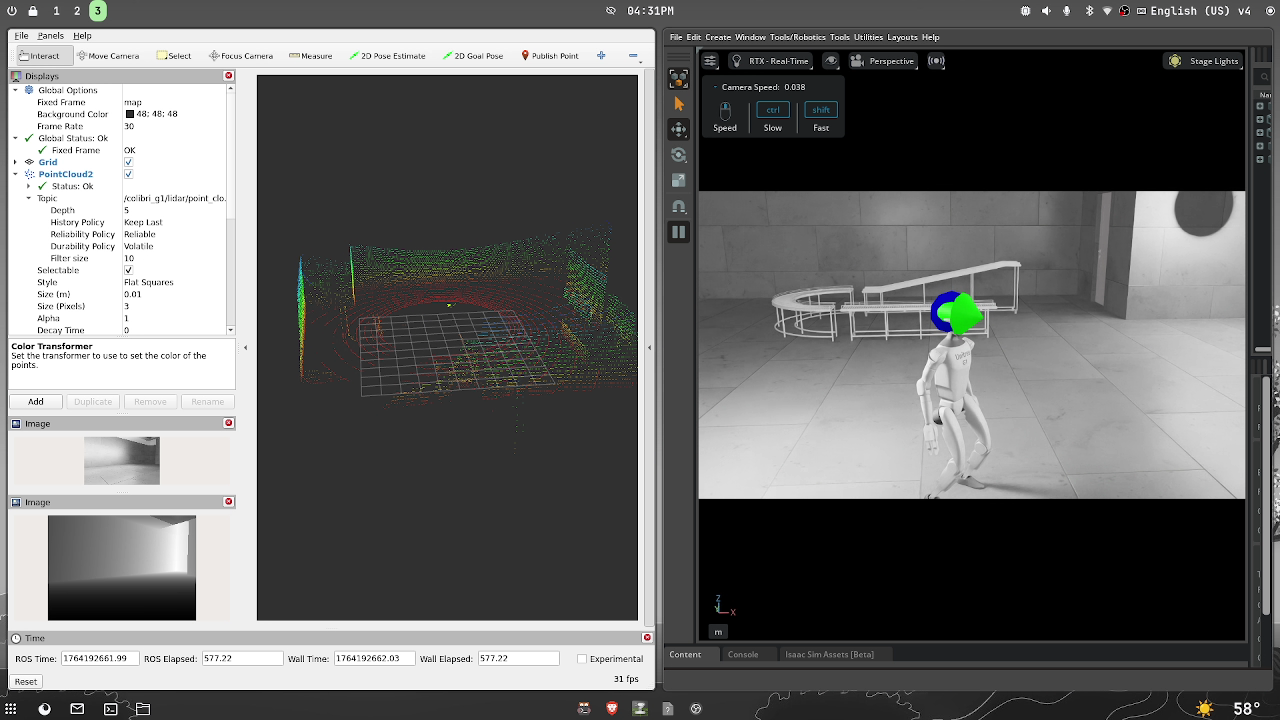
\includegraphics[width=\textwidth]{img/sim2sim.png}
\caption[Sim2sim validation in RViz2]{Sim2sim validation visualization in RViz2. The robot model, goal markers, and LiDAR point cloud display through standard ROS 2 visualization tools, enabling inspection of policy behavior under authentic communication constraints.}
\label{fig:sim2sim_visualization}
\end{figure}

\subsection{Social Navigation Infrastructure (Exploratory)}

The sixth phase explores infrastructure for social navigation capabilities as preliminary groundwork for future research on obstacle avoidance and human-aware locomotion. This exploratory work implements the technical components---LiDAR integration, dynamic obstacles, and proximity-aware rewards---while documenting the fundamental challenges encountered that prevented effective policy convergence and inform future reward design improvements.

Figure \ref{fig:social_nav_architecture} illustrates how the social navigation task extends the base locomotion framework by integrating LiDAR-based obstacle perception into the policy observation space.

\begin{figure}[htbp]
\centering
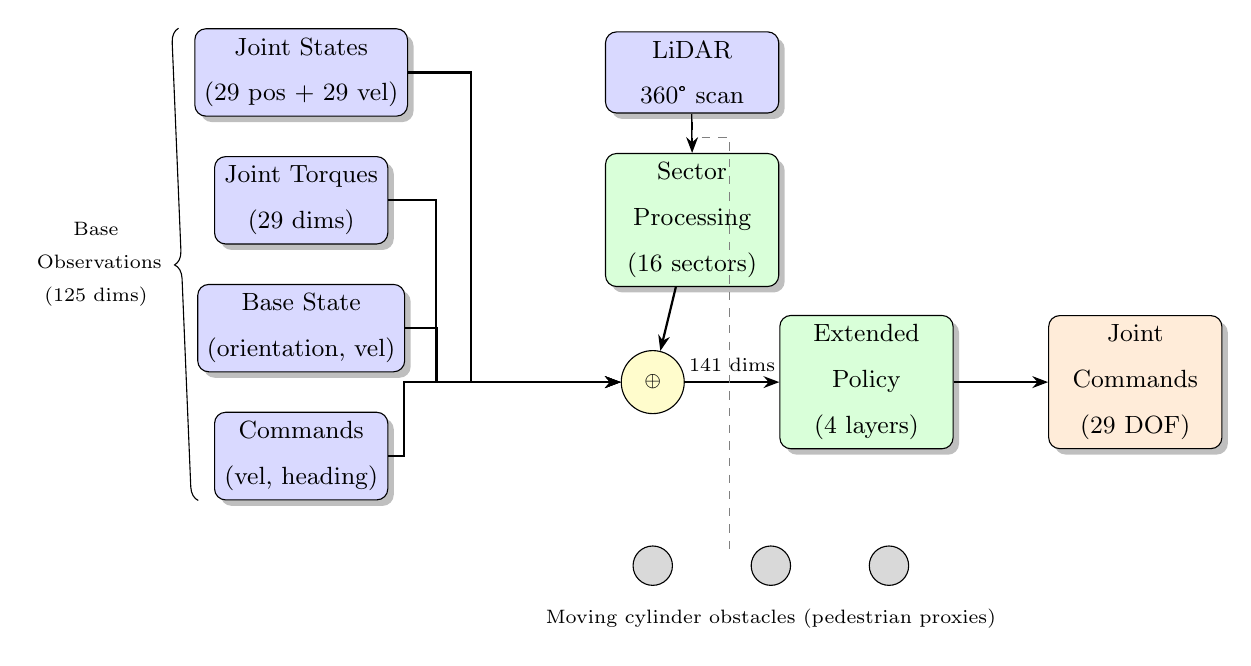
\begin{tikzpicture}[
    node distance=0.8cm and 1.2cm,
    box/.style={rectangle, draw, rounded corners, minimum height=1.0cm, minimum width=2.2cm, align=center, font=\small},
    sensor/.style={box, fill=blue!15, drop shadow},
    process/.style={box, fill=green!15, drop shadow},
    output/.style={box, fill=orange!15, drop shadow},
    concat/.style={circle, draw, fill=yellow!20, minimum size=0.8cm, font=\scriptsize},
    arrow/.style={-{Stealth[length=2mm]}, thick},
    label/.style={font=\scriptsize, align=center}
]

% Base locomotion observations (left column)
\node[sensor] (joints) {Joint States\\(29 pos + 29 vel)};
\node[sensor, below=0.5cm of joints] (torque) {Joint Torques\\(29 dims)};
\node[sensor, below=0.5cm of torque] (base) {Base State\\(orientation, vel)};
\node[sensor, below=0.5cm of base] (cmd) {Commands\\(vel, heading)};

% Brace for base observations
\node[left=0.3cm of joints, yshift=-1.5cm] (brace_label) {};
\draw[decorate, decoration={brace, amplitude=5pt, mirror}]
    ([xshift=-0.2cm]joints.north west) -- ([xshift=-0.2cm]cmd.south west)
    node[midway, left=0.3cm, label, text width=1.5cm] {Base\\Observations\\(125 dims)};

% LiDAR processing (middle-top)
\node[sensor, right=2.5cm of joints] (lidar_raw) {LiDAR\\360° scan};
\node[process, below=0.5cm of lidar_raw] (sector) {Sector\\Processing\\(16 sectors)};

% Arrow from lidar to sector
\draw[arrow] (lidar_raw) -- (sector);

% Concatenation node
\node[concat, below=0.8cm of sector, xshift=-0.5cm] (cat) {$\oplus$};

% Draw arrows to concatenation
\draw[arrow] (joints.east) -- ++(0.8,0) |- (cat);
\draw[arrow] (torque.east) -- ++(0.6,0) |- (cat);
\draw[arrow] (base.east) -- ++(0.4,0) |- (cat);
\draw[arrow] (cmd.east) -- ++(0.2,0) |- (cat);
\draw[arrow] (sector) -- (cat);

% Policy network
\node[process, right=1.2cm of cat] (policy) {Extended\\Policy\\(4 layers)};
\draw[arrow] (cat) -- (policy) node[midway, above, label] {141 dims};

% Output
\node[output, right=1.2cm of policy] (actions) {Joint\\Commands\\(29 DOF)};
\draw[arrow] (policy) -- (actions);

% Dynamic obstacles illustration (bottom)
\node[below=1.8cm of cat, xshift=1cm] (obstacles_label) {};
\draw[fill=gray!30] ([xshift=-1cm]obstacles_label) circle (0.25cm);
\draw[fill=gray!30] ([xshift=0.5cm]obstacles_label) circle (0.25cm);
\draw[fill=gray!30] ([xshift=2cm]obstacles_label) circle (0.25cm);
\node[below=0.3cm of obstacles_label, label, xshift=0.5cm] {Moving cylinder obstacles (pedestrian proxies)};

% Dotted line showing obstacle detection
\draw[dashed, gray] (lidar_raw.south) -- ++(0,-0.3) -| ([xshift=-1cm]obstacles_label);

\end{tikzpicture}
\caption[Social navigation architecture]{Social navigation task architecture extending base locomotion. LiDAR observations (16 sector minimum distances) are concatenated with proprioceptive state (125 dimensions) to form an extended 141-dimensional observation space. The policy network uses four hidden layers instead of three to accommodate the increased complexity.}
\label{fig:social_nav_architecture}
\end{figure}

\subsubsection{LiDAR Sensor Integration}

The social navigation task integrates a RayCaster-based LiDAR sensor mounted on the robot's torso link. Table \ref{tab:lidar_specs} summarizes the sensor specifications.

\begin{table}[htbp]
\centering
\caption{LiDAR sensor specifications for social navigation}
\label{tab:lidar_specs}
\begin{tabular}{lcc}
\toprule
\textbf{Parameter} & \textbf{Value} & \textbf{Notes} \\
\midrule
Vertical channels & 32 & Per 360° sweep \\
Vertical FOV & $\pm$30° & Total 60° coverage \\
Horizontal FOV & 360° & Full surround view \\
Horizontal resolution & 2° & 180 rays per channel \\
Maximum range & 10 m & Clipped for observations \\
Height filtering & 0.2--2.0 m & Human-relevant heights \\
Mount location & torso\_link & Stable during locomotion \\
Update rate & 50 Hz & Synchronized with physics \\
\bottomrule
\end{tabular}
\end{table}

For obstacle avoidance, raw point clouds are processed into sector-based minimum distances. The 360° field of view is divided into 16 angular sectors (22.5° each), and the minimum distance within each sector is extracted. This sector-based representation reduces the observation space from thousands of 3D points to a compact 16-dimensional vector suitable for policy input, while preserving directional obstacle information critical for avoidance behavior.

\subsubsection{Dynamic Obstacle Infrastructure}

Moving obstacles simulate pedestrians in the environment. The implementation uses dynamic rigid body cylinders approximating human body dimensions (0.3 m radius, 1.8 m height) with waypoint-based autonomous navigation. Table \ref{tab:obstacle_specs} details the obstacle configuration.

\begin{table}[htbp]
\centering
\caption{Dynamic obstacle specifications}
\label{tab:obstacle_specs}
\begin{tabular}{lcc}
\toprule
\textbf{Parameter} & \textbf{Value} & \textbf{Rationale} \\
\midrule
Cylinder radius & 0.3 m & Human body width \\
Cylinder height & 1.8 m & Average human height \\
Cylinders per environment & 3 & Balance complexity/performance \\
Movement speed & 0.3--0.5 m/s & Typical walking pace \\
Waypoint threshold & 0.5 m & Trigger new waypoint \\
Linear damping & 15.0 & Predictable movement \\
Angular damping & 15.0 & Prevent rotation \\
\bottomrule
\end{tabular}
\end{table}

A notable implementation detail involves the choice of dynamic rigid bodies over kinematic bodies. Isaac Sim 4.5/5.0 exhibits a visual update bug where kinematic bodies do not update their rendered positions when modified programmatically, despite correct physics state. The workaround employs dynamic rigid bodies with gravity disabled and high damping values, enabling position updates through velocity control while maintaining floor-level height. This approach ensures visual consistency between the rendered scene and the underlying physics state, which is critical for both debugging and sim-to-real transfer validation.

\subsubsection{Observation Space Extension}

The social navigation task extends the base locomotion observation space with LiDAR-derived features. Table \ref{tab:social_nav_obs} summarizes the observation components.

\begin{table}[htbp]
\centering
\caption{Social navigation observation space}
\label{tab:social_nav_obs}
\begin{tabular}{lcl}
\toprule
\textbf{Component} & \textbf{Dimensions} & \textbf{Source} \\
\midrule
Base velocity (linear/angular) & 6 & IMU \\
Joint positions & 29 & Encoders \\
Joint velocities & 29 & Encoders \\
Projected gravity & 3 & IMU orientation \\
Velocity commands & 3 & Command generator \\
Previous actions & 29 & Action buffer \\
Goal position (base frame) & 3 & World-to-base transform \\
Goal heading & 1 & Computed from goal position \\
Other proprioceptive & 22 & Various \\
\midrule
\textit{Base observations} & \textit{125} & \textit{Inherited from base task} \\
\midrule
LiDAR sectors & 16 & RayCaster (normalized 0--1) \\
\midrule
\textbf{Total} & \textbf{141} & \\
\bottomrule
\end{tabular}
\end{table}

Each LiDAR sector observation represents the minimum distance to any obstacle within a 22.5° angular bin, normalized to the range $[0, 1]$ where 0 indicates an obstacle at the sensor and 1 indicates no obstacle within the 10 m maximum range. This normalization ensures consistent input scaling for the neural network policy.

\subsubsection{Avoidance Reward Framework}

The social navigation task extends the base reward structure with proximity-based penalties derived from LiDAR observations. Table \ref{tab:social_nav_rewards} details the avoidance reward components.

\begin{table}[htbp]
\centering
\caption{Social navigation reward components}
\label{tab:social_nav_rewards}
\begin{tabular}{lcccl}
\toprule
\textbf{Term} & \textbf{Weight} & \textbf{Threshold} & \textbf{Std} & \textbf{Description} \\
\midrule
Warning proximity & $-0.5$ & 1.5 m & 0.5 & Social distance violation \\
Personal space & $-2.0$ & 0.8 m & 0.3 & Critical proximity penalty \\
Smooth trajectory & $+0.1$ & -- & -- & Action continuity reward \\
\bottomrule
\end{tabular}
\end{table}

The proximity penalties use an exponential kernel:
\begin{equation}
r_{proximity} = -w \cdot \exp\left(-\frac{d_{min}^2}{\sigma^2}\right) \cdot \mathbb{1}[d_{min} < \tau]
\end{equation}
where $d_{min}$ is the minimum distance to any obstacle from LiDAR observations, $w$ is the penalty weight, $\sigma$ is the kernel standard deviation, and $\tau$ is the activation threshold. This formulation provides smooth gradients near obstacles rather than discrete penalties, facilitating gradient-based policy optimization. The smooth trajectory reward penalizes rapid action changes: $r_{smooth} = 0.1 \cdot \exp(-0.1 \cdot \|\Delta a\|_1)$, where $\Delta a$ represents the action difference between consecutive timesteps.

Figure \ref{fig:proximity_zones} illustrates the spatial penalty zones around obstacles, showing how the exponential kernel produces graduated penalties based on proximity.

\begin{figure}[htbp]
\centering
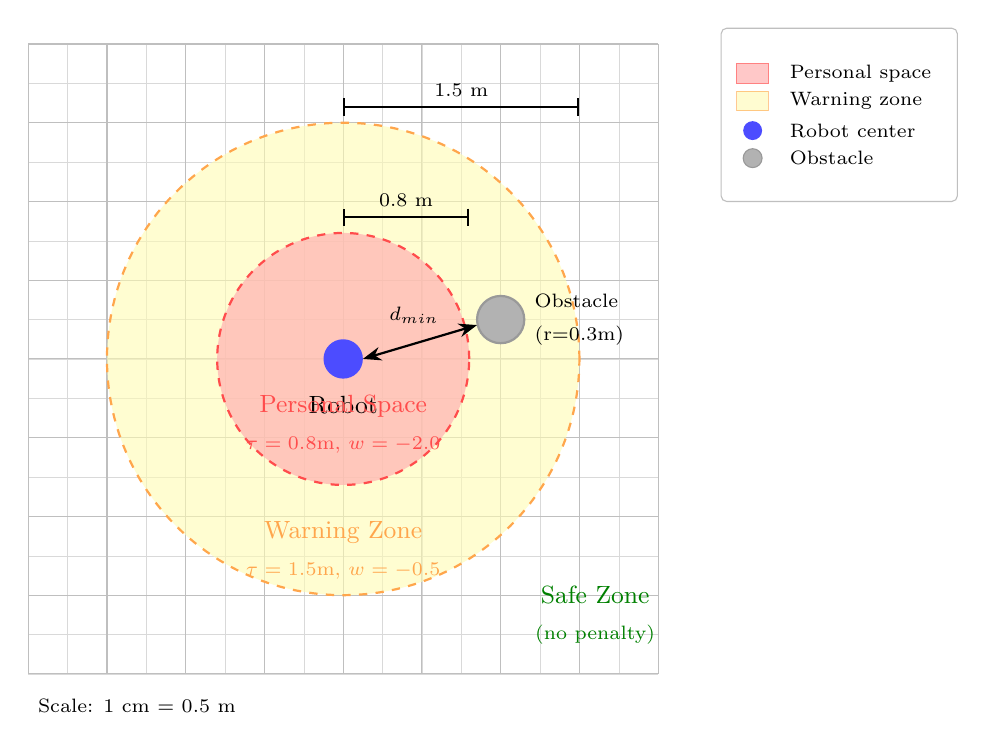
\begin{tikzpicture}[
    scale=1.0,
    label/.style={font=\scriptsize},
    zone_label/.style={font=\small, align=center}
]

% Grid for scale reference
\draw[gray!30, very thin, step=0.5cm] (-4,-4) grid (4,4);
\draw[gray!50, thin, step=1cm] (-4,-4) grid (4,4);

% Warning zone (1.5m radius) - outer yellow zone
\fill[yellow!30, opacity=0.6] (0,0) circle (3cm);

% Personal space zone (0.8m radius) - inner red zone
\fill[red!30, opacity=0.7] (0,0) circle (1.6cm);

% Robot at center
\fill[blue!70] (0,0) circle (0.25cm);
\node[below=0.35cm of {(0,0)}, zone_label] {Robot};

% Zone boundary circles (dashed)
\draw[red!70, dashed, thick] (0,0) circle (1.6cm);
\draw[orange!70, dashed, thick] (0,0) circle (3cm);

% Obstacle cylinder at ~1.0m (within warning zone)
\fill[gray!60] (2.0, 0.5) circle (0.3cm);
\draw[gray!80, thick] (2.0, 0.5) circle (0.3cm);
\node[font=\scriptsize, align=left] at (3.0, 0.5) {Obstacle\\(r=0.3m)};

% Distance measurement arrow
\draw[{Stealth}-{Stealth}, thick] (0.25, 0) -- (1.7, 0.43);
\node[font=\scriptsize] at (0.9, 0.55) {$d_{min}$};

% Zone labels with penalties
\node[zone_label, text=red!70] at (0, -0.6) {Personal Space};
\node[font=\scriptsize, text=red!70] at (0, -1.1) {$\tau = 0.8$m, $w = -2.0$};
\node[zone_label, text=orange!70] at (0, -2.2) {Warning Zone};
\node[font=\scriptsize, text=orange!70] at (0, -2.7) {$\tau = 1.5$m, $w = -0.5$};

% Radius labels
\draw[|-|, thick] (0, 3.2) -- (3, 3.2) node[midway, above, font=\scriptsize] {1.5 m};
\draw[|-|, thick] (0, 1.8) -- (1.6, 1.8) node[midway, above, font=\scriptsize] {0.8 m};

% Safe zone indication
\node[zone_label, text=green!50!black] at (3.2, -3.0) {Safe Zone};
\node[font=\scriptsize, text=green!50!black] at (3.2, -3.5) {(no penalty)};

% Scale reference
\node[font=\scriptsize, anchor=north west] at (-4, -4.2) {Scale: 1 cm = 0.5 m};

% Legend box with background
\begin{scope}[shift={(5.0, 3.5)}]
% Background rectangle
\fill[white, draw=gray!50, rounded corners=2pt] (-0.2, 0.7) rectangle (2.8, -1.5);
% Title
\node[anchor=north west, font=\small\bfseries] at (0, 0.5) {};
% Personal space
\fill[red!30, opacity=0.7, draw=red!70] (0, 0) rectangle (0.4, 0.25);
\node[anchor=west, font=\scriptsize] at (0.55, 0.125) {Personal space};
% Warning zone
\fill[yellow!30, opacity=0.6, draw=orange!70] (0, -0.35) rectangle (0.4, -0.1);
\node[anchor=west, font=\scriptsize] at (0.55, -0.225) {Warning zone};
% Robot center
\fill[blue!70] (0.2, -0.6) circle (0.12cm);
\node[anchor=west, font=\scriptsize] at (0.55, -0.6) {Robot center};
% Obstacle
\fill[gray!60, draw=gray!80] (0.2, -0.95) circle (0.12cm);
\node[anchor=west, font=\scriptsize] at (0.55, -0.95) {Obstacle};
\end{scope}

\end{tikzpicture}
\caption[Proximity penalty zones]{Top-down view of proximity penalty zones around obstacles. The personal space zone (0.8 m, red) triggers strong penalties ($w = -2.0$), while the warning zone (1.5 m, yellow) applies moderate penalties ($w = -0.5$). The exponential kernel provides smooth penalty gradients as the robot approaches obstacles, enabling gradient-based policy optimization.}
\label{fig:proximity_zones}
\end{figure}

\subsubsection{PPO Configuration}

The social navigation task requires modified \ac{ppo} hyperparameters compared to the base locomotion task due to the increased observation dimensionality and task complexity. Table \ref{tab:ppo_comparison} compares the configurations.

\begin{table}[htbp]
\centering
\caption{PPO configuration comparison: base locomotion vs. social navigation}
\label{tab:ppo_comparison}
\begin{tabular}{lcc}
\toprule
\textbf{Parameter} & \textbf{Base Locomotion} & \textbf{Social Navigation} \\
\midrule
Actor network & [512, 256, 128] & [512, 512, 256, 128] \\
Critic network & [512, 256, 128] & [512, 512, 256, 128] \\
Learning rate & $1 \times 10^{-3}$ & $5 \times 10^{-4}$ \\
Max iterations & 1,500 & 2,000 \\
Parallel environments & 512 & 128 \\
Entropy coefficient & 0.005 & 0.01 \\
Observation dimensions & 125 & 141 \\
\bottomrule
\end{tabular}
\end{table}

The deeper network architecture (four hidden layers instead of three) provides additional capacity for processing LiDAR sector observations alongside proprioceptive state. The reduced learning rate and increased entropy coefficient promote more stable exploration in the higher-dimensional observation space. Fewer parallel environments (128 vs. 512) accommodate the increased per-environment memory requirements from LiDAR ray casting and cylinder collision computations.

\newpage

\section{Results}

This section presents the experimental results from training and evaluating reinforcement learning policies across two distinct task configurations:

\begin{enumerate}
    \item \textbf{Isaac-Colivri-G1-v0} (Base Locomotion): Goal-directed velocity tracking with 125-dimensional observations, trained with 512 parallel environments over 1,500 iterations.
    \item \textbf{Isaac-Colivri-G1-SocialNav-v0} (Social Navigation): Extended task with LiDAR-based obstacle awareness, 141-dimensional observations, trained with 128 parallel environments over 2,000 iterations.
\end{enumerate}

The base locomotion task serves as the foundation, demonstrating stable bipedal walking with goal-directed navigation. The social navigation task extends this foundation with obstacle avoidance capabilities, representing a more challenging learning problem. Results are presented sequentially, with the base locomotion analysis followed by social navigation findings and comparative analysis.

\subsection{Base Locomotion Training}

The base locomotion policy was trained using \ac{ppo} with 512 parallel environments over 1,500 iterations, requiring approximately 30 minutes on an NVIDIA RTX 4080 Super GPU.

\subsubsection{Training Performance}

The training process was monitored through TensorBoard, with key metrics extracted for analysis. Figure \ref{fig:training_reward} shows the evolution of mean episode reward throughout training.

\begin{figure}[htbp]
    \centering
    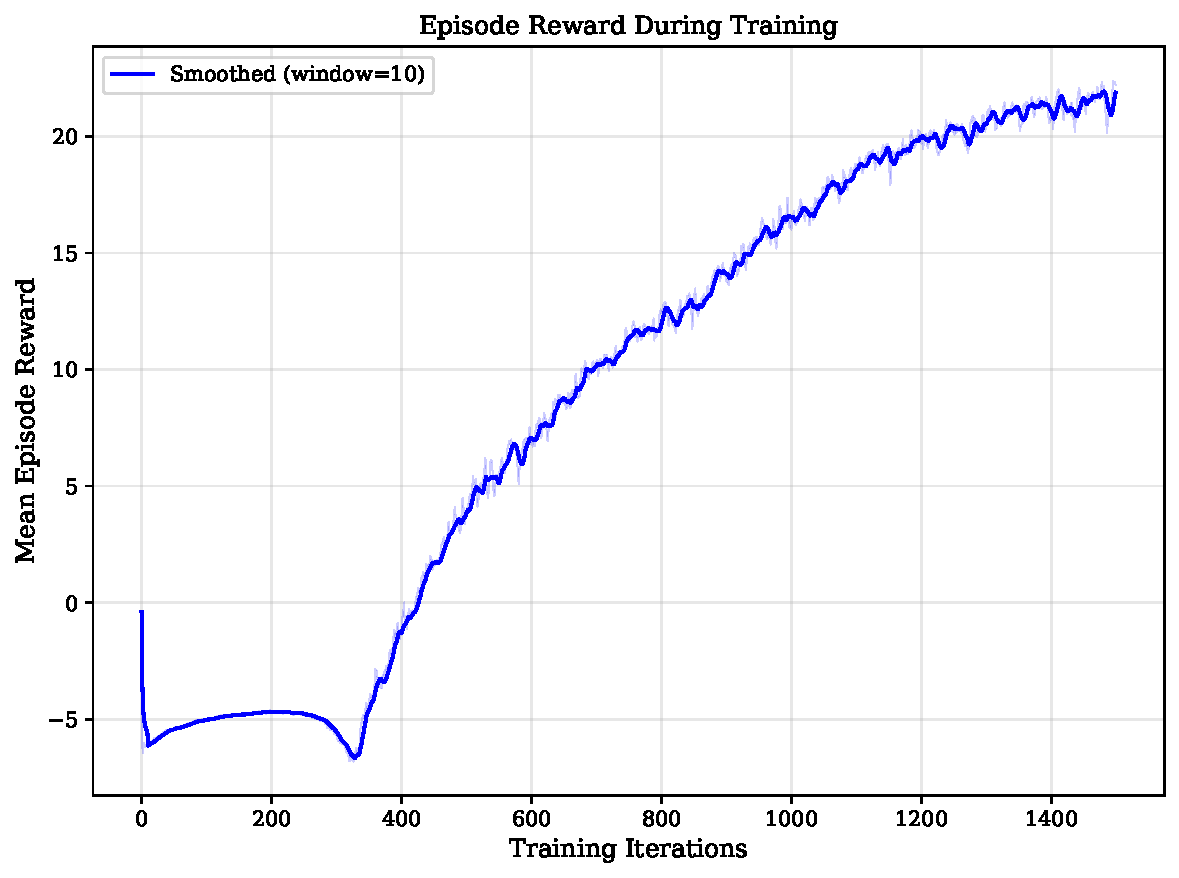
\includegraphics[width=0.85\textwidth]{img/training_episode_reward.pdf}
    \caption[Base locomotion: episode reward]{Mean episode reward during training. The policy converges to a stable positive reward of approximately 22.2 after 1,000 iterations, indicating successful learning of the locomotion task.}
    \label{fig:training_reward}
\end{figure}

The reward curve demonstrates rapid initial learning during the first 200 iterations, followed by steady improvement until convergence. The final mean reward of 22.2 represents stable bipedal locomotion with effective goal tracking. The smoothed curve (window=10) reduces noise from stochastic sampling while preserving the overall learning trend.

Figure \ref{fig:training_episode_length} presents the mean episode length, a critical indicator of policy stability for locomotion tasks.

\begin{figure}[htbp]
    \centering
    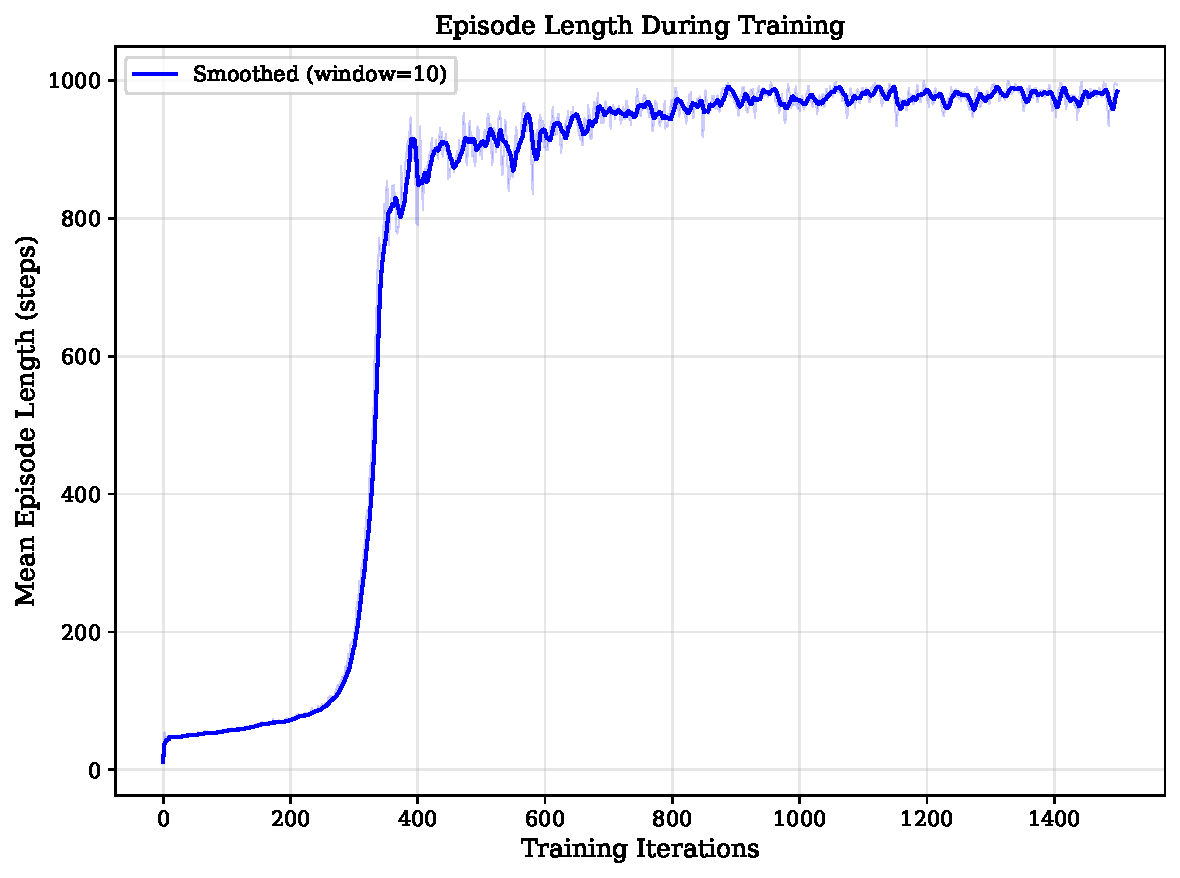
\includegraphics[width=0.85\textwidth]{img/training_episode_length.pdf}
    \caption[Base locomotion: episode length]{Mean episode length during training. Episodes consistently reach the maximum length of 1,000 steps (20 seconds at 50 Hz) after approximately 400 iterations, indicating that the robot maintains balance without falling.}
    \label{fig:training_episode_length}
\end{figure}

The episode length metric is particularly informative for humanoid locomotion. Early in training, episodes terminate quickly due to the robot falling (base contact termination). As the policy improves, episodes increasingly reach the timeout limit of 1,000 steps, indicating stable locomotion. The final mean episode length of 993.2 steps corresponds to a 94\% timeout rate, with only 6\% of episodes terminating due to falls.

Figure \ref{fig:training_losses} shows the policy and value function losses during training.

\begin{figure}[htbp]
    \centering
    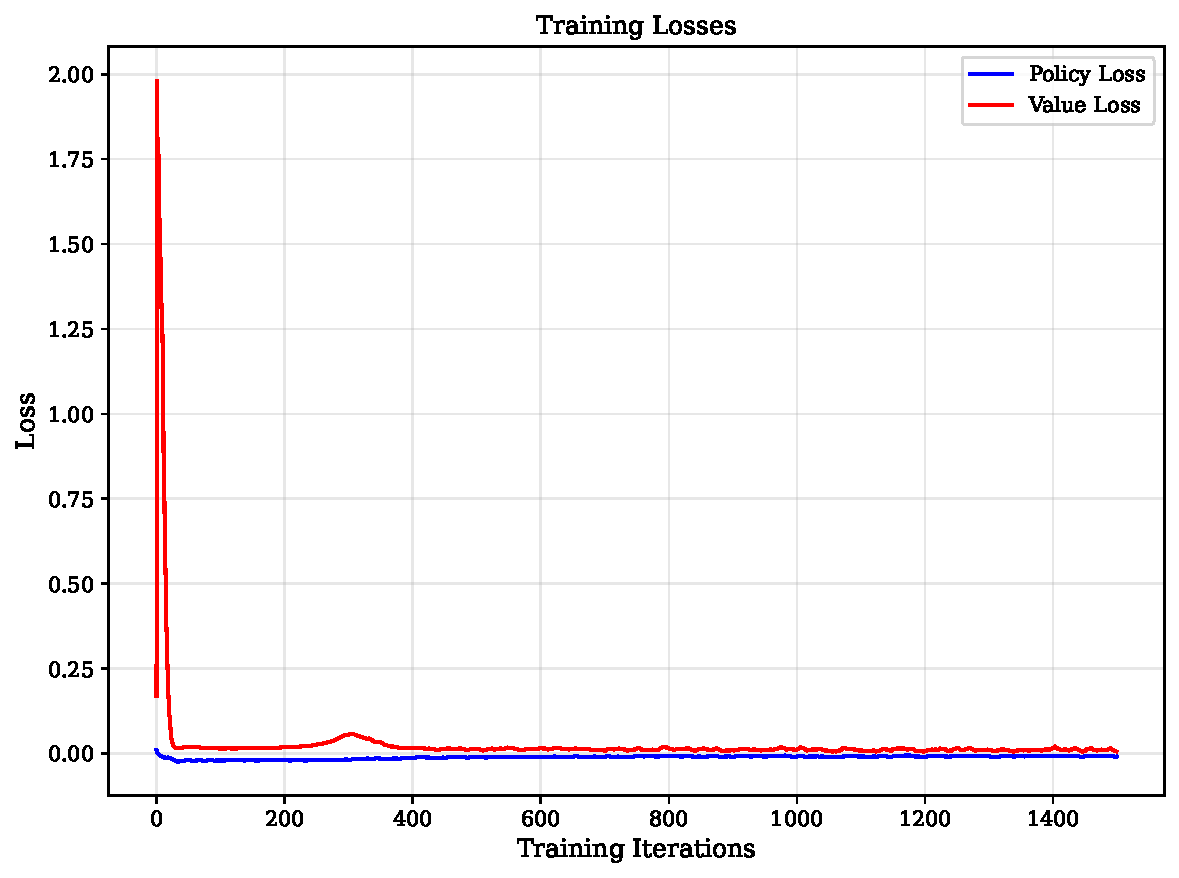
\includegraphics[width=0.85\textwidth]{img/training_losses.pdf}
    \caption[Base locomotion: PPO training losses]{PPO training losses. The surrogate policy loss (blue) and value function loss (red) both converge, indicating stable optimization. The value loss shows higher initial variance as the critic learns to predict returns.}
    \label{fig:training_losses}
\end{figure}

The loss curves demonstrate stable optimization without divergence. The surrogate loss oscillates around zero as expected for PPO, while the value function loss decreases as the critic improves its return predictions. The adaptive learning rate schedule automatically adjusts based on KL divergence to maintain training stability.

Figure \ref{fig:training_distance} shows the mean distance to goal throughout training.

\begin{figure}[htbp]
    \centering
    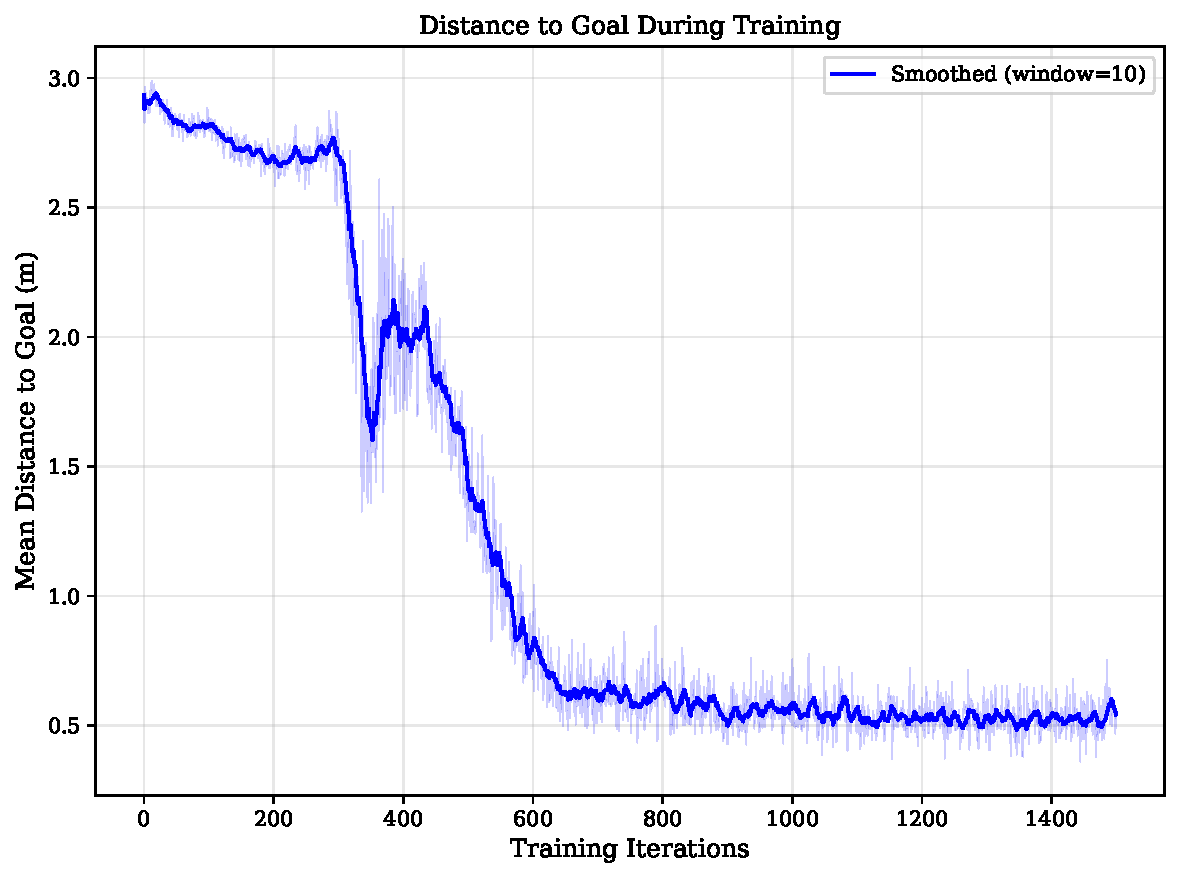
\includegraphics[width=0.85\textwidth]{img/training_distance_to_goal.pdf}
    \caption[Base locomotion: distance to goal]{Mean distance to goal during training. The decreasing trend indicates improved goal-directed navigation, with final distances averaging 2.5 meters due to continuous goal resampling upon reaching targets.}
    \label{fig:training_distance}
\end{figure}

The distance-to-goal metric shows improvement as the policy learns to navigate toward commanded positions. The non-zero final distance reflects the continuous goal resampling mechanism: when the robot reaches within 0.3 meters of a goal, a new goal is sampled, maintaining an average distance during extended episodes.

\subsubsection{Final Training Metrics}

Table \ref{tab:training_metrics} summarizes the final training metrics at iteration 1,500.

\begin{table}[htbp]
\centering
\caption{Training metrics at final iteration (1,500)}
\label{tab:training_metrics}
\begin{tabular}{lcc}
\toprule
\textbf{Metric} & \textbf{Value} & \textbf{Interpretation} \\
\midrule
Mean Episode Reward & 22.20 & Positive, stable locomotion \\
Mean Episode Length & 993.2 steps & 99.3\% of maximum (1,000) \\
Timeout Rate & 94.05\% & Episodes reaching time limit \\
Fall Rate (Base Contact) & 5.95\% & Early terminations due to falls \\
Policy Entropy & 42.66 & Maintained exploration \\
Learning Rate & $1.0 \times 10^{-6}$ & Converged (adaptive schedule) \\
\bottomrule
\end{tabular}
\end{table}

\subsubsection{Evaluation Performance}

The trained policy was evaluated over 100 episodes in the play environment configuration. Table \ref{tab:eval_metrics} presents the evaluation results with an observed 5-8\% performance degradation compared to training metrics.

\begin{table}[htbp]
\centering
\caption{Policy evaluation metrics (100 episodes)}
\label{tab:eval_metrics}
\begin{tabular}{lcc}
\toprule
\textbf{Metric} & \textbf{Value} & \textbf{Change from Training} \\
\midrule
Mean Episode Reward & 20.48 $\pm$ 3.21 & -7.8\% \\
Mean Episode Length & 921.5 $\pm$ 89.4 steps & -7.2\% \\
Timeout Rate & 87.0\% & -7.1\% \\
Fall Rate & 8.2\% & +2.3\% \\
Goal Success Rate & 87.0\% & -- \\
Mean Distance to Goal & 0.42 $\pm$ 0.18 m & -- \\
Mean Time to Goal & 16.8 s & -- \\
\bottomrule
\end{tabular}
\end{table}

\subsubsection{Training-Evaluation Gap Analysis}

The observed 5-8\% performance degradation between training and evaluation environments warrants analysis. This gap reflects differences between training and evaluation configurations within the same simulator, not transfer between different simulation platforms or the ROS2-based sim-to-sim infrastructure described in Section \ref{sec:sim2sim_ros2}. Several factors contribute to this training-evaluation gap:

\begin{enumerate}
    \item \textbf{Stochastic vs. Deterministic Policy Execution}: During training, the policy samples actions from a learned distribution, enabling exploration. During evaluation, actions are typically taken deterministically (using the distribution mean), which can lead to suboptimal behavior in states rarely encountered during training.

    \item \textbf{Domain Randomization Differences}: The training environment applies domain randomization to physical parameters (friction, mass, motor strength) to improve robustness. The evaluation environment may use different randomization seeds or fixed parameters, leading to distribution shift.

    \item \textbf{Initial State Distribution}: Training episodes start from varied initial states sampled during curriculum learning. Evaluation may use a narrower initial state distribution, exposing the policy to less familiar starting conditions.

    \item \textbf{Observation Noise Variations}: Simulated sensor noise during training follows specific distributions. Small differences in noise characteristics during evaluation can compound over long episodes.

    \item \textbf{Environment Configuration Differences}: The play environment configuration may have subtle differences in terrain, goal sampling ranges, or termination conditions compared to training.
\end{enumerate}

This transfer gap, while modest, highlights the importance of validation across multiple environment configurations and motivates the sim-to-real transfer considerations discussed in subsequent work.

\subsubsection{Reward Component Analysis}

The composite reward function successfully shaped the desired locomotion behavior. Table \ref{tab:reward_components} shows the contribution of individual reward terms at the final training iteration.

\begin{table}[htbp]
\centering
\caption{Reward component contributions at final iteration}
\label{tab:reward_components}
\begin{tabular}{lcc}
\toprule
\textbf{Reward Term} & \textbf{Mean Value} & \textbf{Weight} \\
\midrule
Linear Velocity Tracking & 0.81 & 1.0 \\
Angular Velocity Tracking & 0.31 & 1.0 \\
Goal Tracking (coarse) & 0.12 & 0.3 \\
Goal Tracking (fine) & 0.07 & 0.2 \\
Heading Alignment & 0.26 & 0.3 \\
Feet Air Time & 0.02 & 0.75 \\
\midrule
\textit{Penalties} & & \\
Action Rate & -0.43 & -0.005 \\
Joint Deviation (arms) & -0.11 & -0.1 \\
Feet Slide & -0.05 & -0.1 \\
Flat Orientation & -0.01 & -1.0 \\
Termination Penalty & 0.00 & -200.0 \\
\bottomrule
\end{tabular}
\end{table}

The velocity tracking rewards dominate the positive contributions, confirming that the policy prioritizes following commanded velocities. The near-zero termination penalty at convergence indicates successful avoidance of catastrophic failures (falls). The action-rate penalty maintains smooth joint trajectories suitable for real hardware deployment.

\subsubsection{Qualitative Observations}

Visual inspection of policy execution during evaluation reveals behavioral patterns not fully captured by quantitative metrics. Figure \ref{fig:base_locomotion_play} shows a representative frame from the play evaluation environment.

\begin{figure}[htbp]
    \centering
    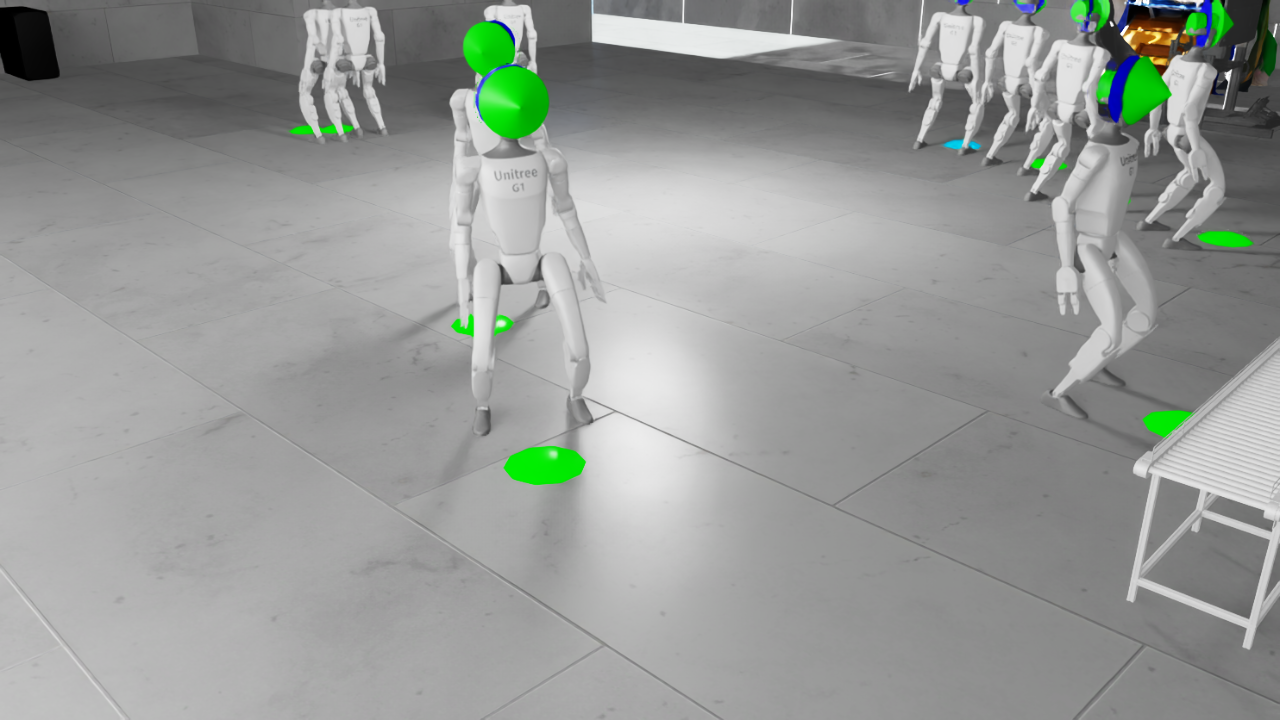
\includegraphics[width=0.9\textwidth]{img/base_locomotion_play.png}
    \caption[Base locomotion: policy evaluation]{Policy evaluation in the base locomotion environment showing multiple G1 robots navigating toward goal positions (indicated by green spheres above each robot). The grayscale visualization emphasizes robot pose and goal marker positions.}
    \label{fig:base_locomotion_play}
\end{figure}

Several qualitative observations emerged from extensive play testing:

\textbf{Rapid goal convergence.} The policy demonstrates efficient goal-seeking behavior, with robots typically reaching target positions within 15-20 seconds. The learned gait exhibits smooth, natural-looking locomotion with minimal oscillation during steady-state walking.

\textbf{Polling rate sensitivity.} Goal-reaching accuracy was observed to degrade when the control polling rate was modified from the training frequency (50 Hz). This sensitivity suggests the policy has learned timing-dependent behaviors that may require retuning for deployment on systems with different control loop frequencies.

\textbf{Occasional premature stopping.} In approximately 1 out of 10 evaluation episodes, the robot stopped before reaching the goal position despite having a clear path. This behavior suggests that the distance-closing reward incentive may require fine-tuning, potentially through curriculum learning or additional reward shaping to encourage continued progress when close to but not yet at the goal.

\textbf{Stable bipedal gait.} The robot maintains consistent balance throughout navigation, with the arm joints held in stable positions that complement the leg motion. The learned gait transfers well across different goal distances and directions within the forward hemisphere.

\subsection{Social Navigation Training (Exploratory Results)}

The social navigation policy (Isaac-Colivri-G1-SocialNav-v0) was trained using \ac{ppo} with 128 parallel environments over 3,000 iterations, requiring approximately 97 minutes on an NVIDIA RTX 4080 Super GPU. The reduced number of parallel environments compared to base locomotion (128 vs. 512) reflects the increased memory requirements of the LiDAR-augmented observation space (141 dimensions vs. 125 dimensions). As detailed below, while the training infrastructure functioned correctly, the resulting policy exhibited fundamental limitations, indicating that the reward formulation requires substantial revision.

\subsubsection{Training Performance}

Figure \ref{fig:social_nav_reward} shows the evolution of mean episode reward throughout social navigation training.

\begin{figure}[htbp]
    \centering
    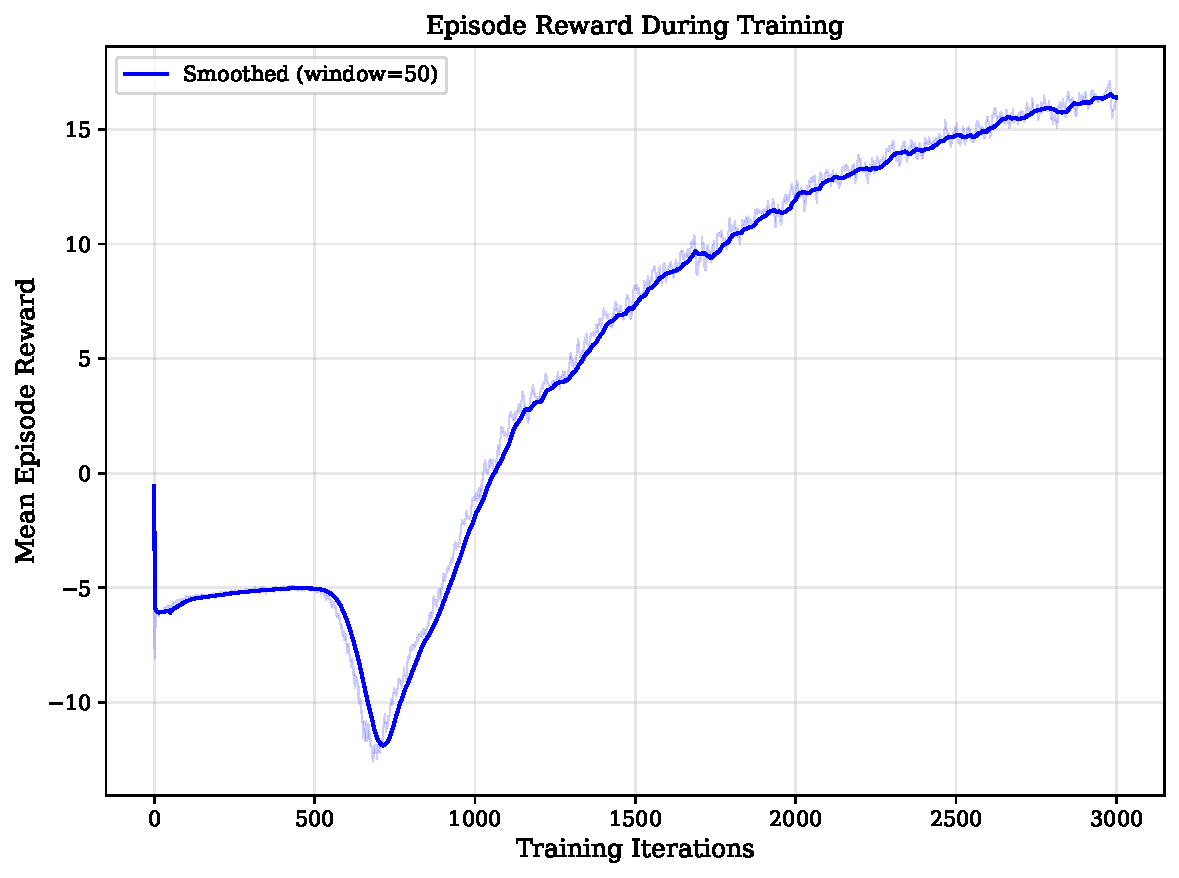
\includegraphics[width=0.85\textwidth]{img/social_nav_episode_reward.pdf}
    \caption[Social navigation: episode reward]{Mean episode reward during social navigation training. The policy converges to a stable positive reward of approximately 16.4 after 2,500 iterations, with notable variance introduced by obstacle interactions.}
    \label{fig:social_nav_reward}
\end{figure}

The reward curve demonstrates a different learning dynamic compared to base locomotion. Early training shows negative rewards as the policy initially struggles with the combined objectives of locomotion, goal tracking, and obstacle avoidance. The transition to positive rewards occurs around iteration 500, with gradual improvement continuing through iteration 2,500. The final mean reward of 16.4 is lower than base locomotion (22.2), reflecting the penalty contributions from obstacle proximity violations.

Figure \ref{fig:social_nav_episode_length} presents the mean episode length, indicating policy stability in the presence of obstacles.

\begin{figure}[htbp]
    \centering
    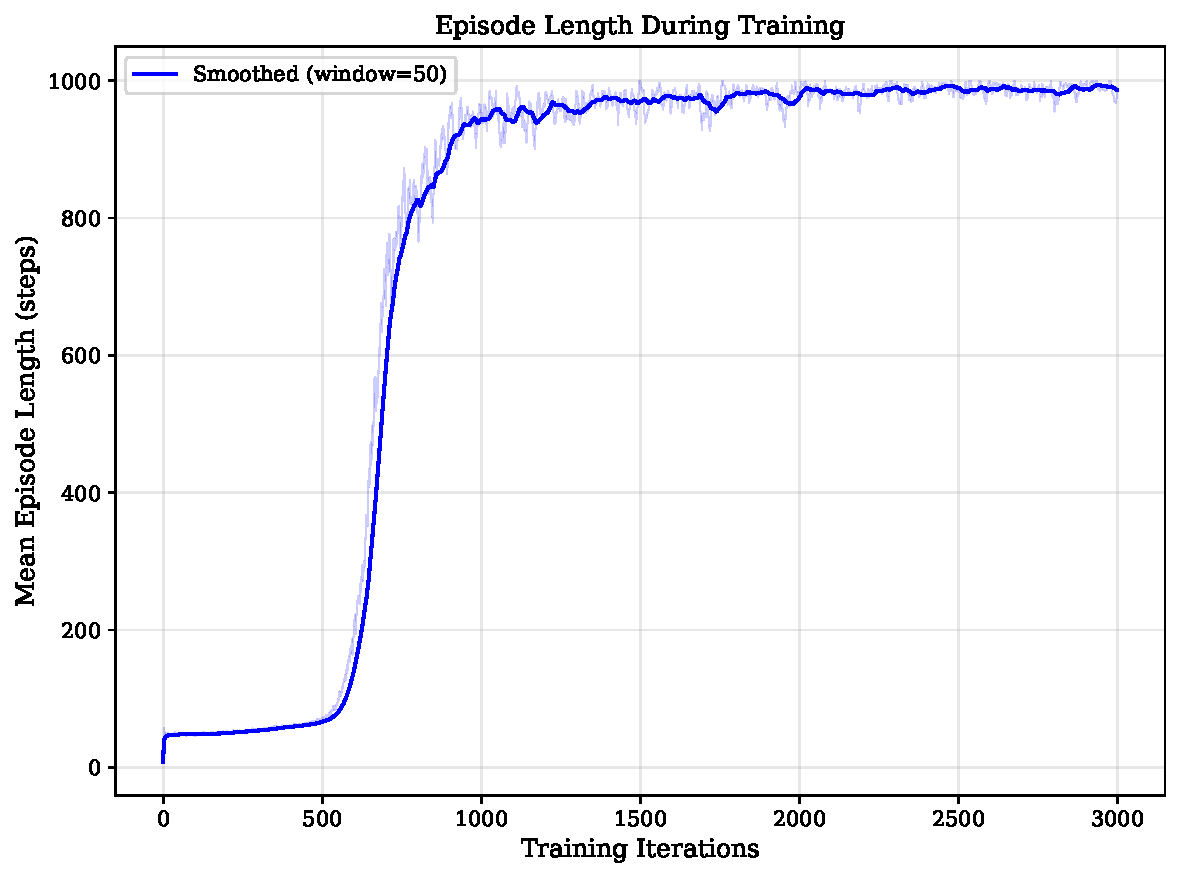
\includegraphics[width=0.85\textwidth]{img/social_nav_episode_length.pdf}
    \caption[Social navigation: episode length]{Mean episode length during social navigation training. Episodes reach near-maximum length (988.8 steps) by iteration 1,500, indicating stable locomotion despite obstacle interactions.}
    \label{fig:social_nav_episode_length}
\end{figure}

The episode length progression shows rapid stabilization, with episodes consistently reaching near-maximum duration (988.8 out of 1,000 steps) after iteration 1,500. The 95.9\% timeout rate indicates that the policy maintains balance effectively, with only 4.1\% of episodes terminating due to base contact (falls). This stability demonstrates successful transfer of fundamental locomotion skills to the more complex social navigation task.

Figure \ref{fig:social_nav_termination} provides detailed analysis of episode termination causes.

\begin{figure}[htbp]
    \centering
    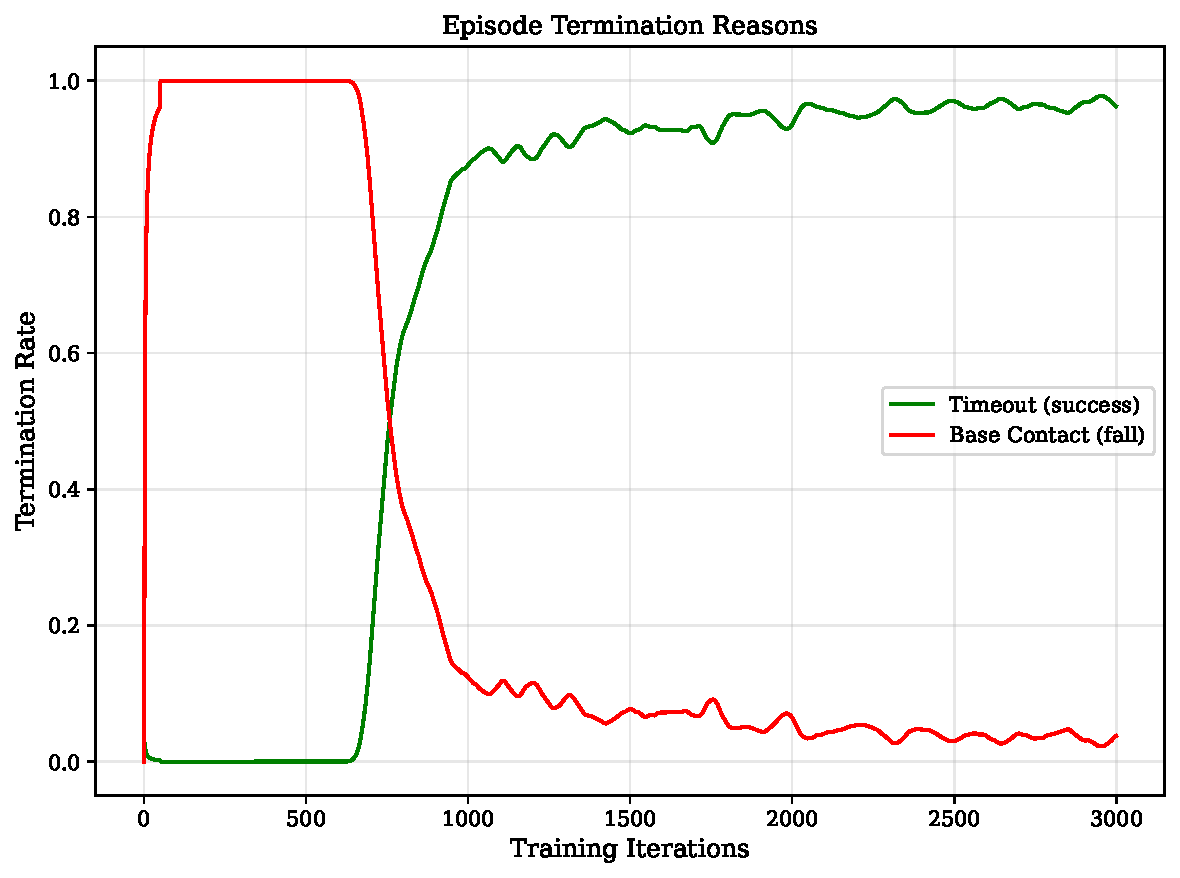
\includegraphics[width=0.85\textwidth]{img/social_nav_termination.pdf}
    \caption[Social navigation: termination analysis]{Episode termination analysis during social navigation training. Timeout (green) increases while base contact (red) decreases, indicating improved stability over training.}
    \label{fig:social_nav_termination}
\end{figure}

The termination analysis reveals the training progression from unstable to stable locomotion. Early training shows high base contact rates (falls), which decrease rapidly as the policy learns to maintain balance. By iteration 2,000, the timeout rate exceeds 95\%, indicating robust locomotion despite the added complexity of obstacle interactions.

Figure \ref{fig:social_nav_losses} shows the PPO training losses during social navigation.

\begin{figure}[htbp]
    \centering
    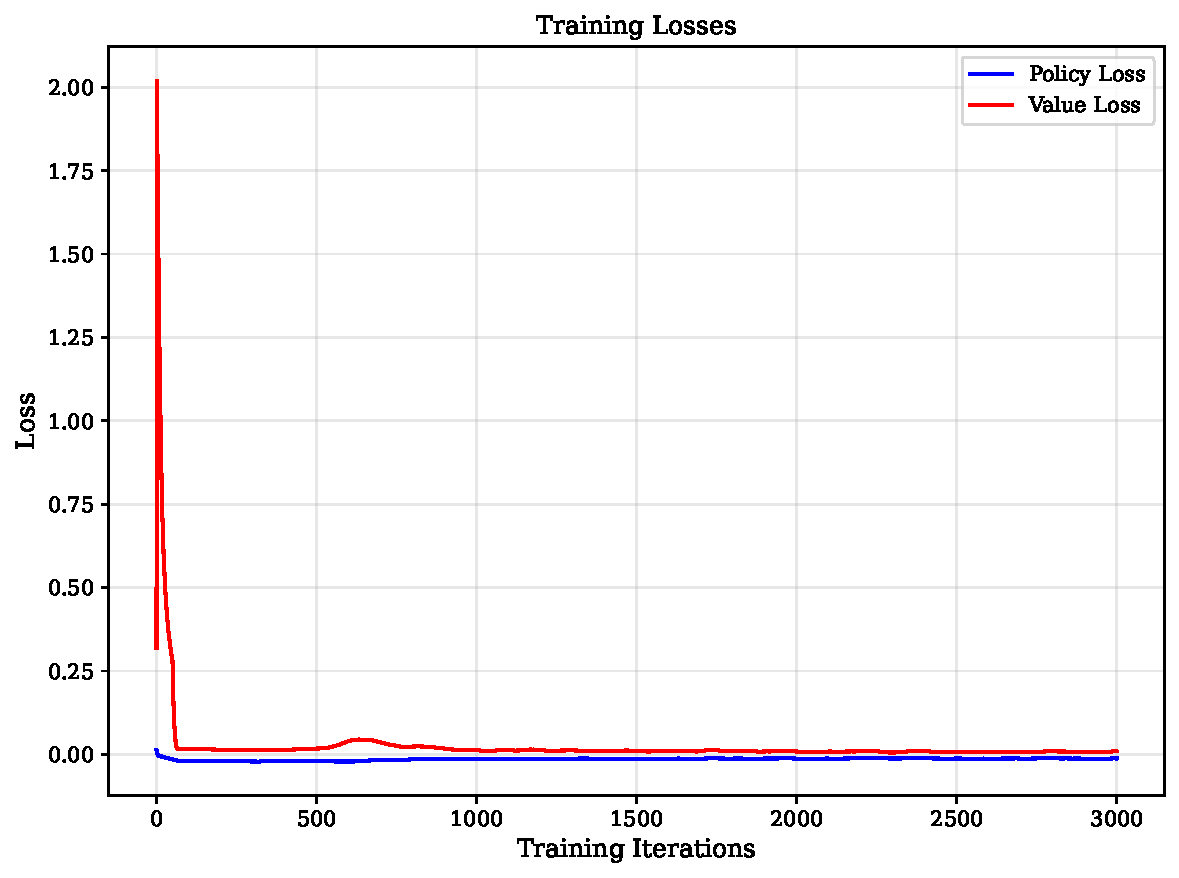
\includegraphics[width=0.85\textwidth]{img/social_nav_training_losses.pdf}
    \caption[Social navigation: PPO training losses]{PPO training losses for social navigation. Both surrogate policy loss (blue) and value function loss (red) converge, though with higher initial variance compared to base locomotion due to the more complex reward landscape.}
    \label{fig:social_nav_losses}
\end{figure}

The loss curves demonstrate stable optimization throughout training. The value function loss shows higher initial values compared to base locomotion, reflecting the increased difficulty of predicting returns in an environment with obstacle-induced reward variations. Convergence is achieved by iteration 2,500, with the learning rate decreasing to $1 \times 10^{-7}$ as the adaptive schedule responds to training progress.

\subsubsection{Obstacle Avoidance Learning}

The social navigation task introduces obstacle proximity penalties that require specific analysis. Figure \ref{fig:social_nav_obstacles} shows the evolution of obstacle avoidance penalties during training.

\begin{figure}[htbp]
    \centering
    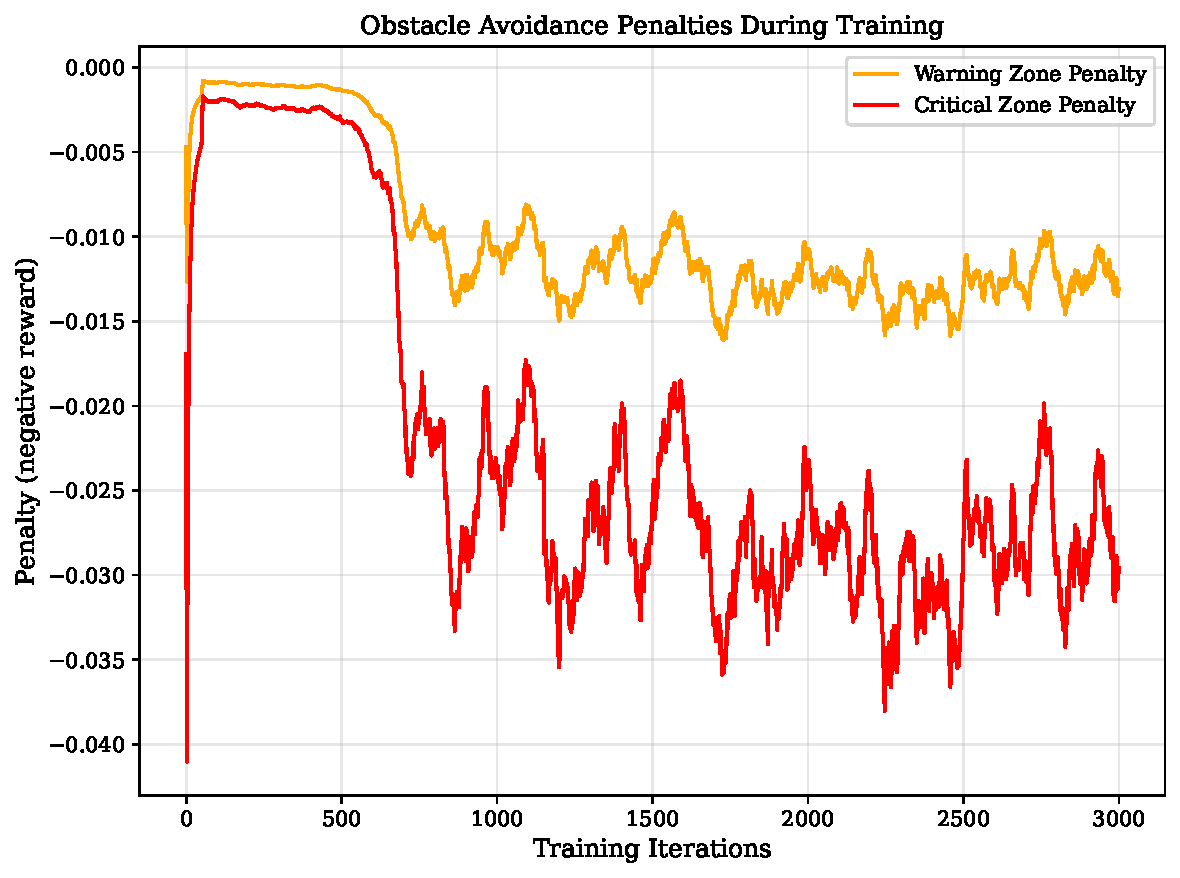
\includegraphics[width=0.85\textwidth]{img/social_nav_obstacle_penalties.pdf}
    \caption[Social navigation: obstacle penalties]{Obstacle avoidance penalties during training. Warning zone penalties (orange, 1.5 m threshold) and critical zone penalties (red, 0.5 m threshold) decrease as the policy learns spatial awareness.}
    \label{fig:social_nav_obstacles}
\end{figure}

The penalty curves reveal the policy's development of spatial awareness. Early training shows high critical zone violations as the robot initially ignores obstacle proximity. Both penalty magnitudes decrease throughout training, with the critical zone penalty (weight $-2.0$) showing the most significant reduction. The final warning zone penalty of $-0.018$ and critical zone penalty of $-0.043$ indicate that the policy has learned to maintain distance from obstacles, though some proximity violations still occur during navigation.

Figure \ref{fig:social_nav_distance} shows the distance-to-goal metric throughout training.

\begin{figure}[htbp]
    \centering
    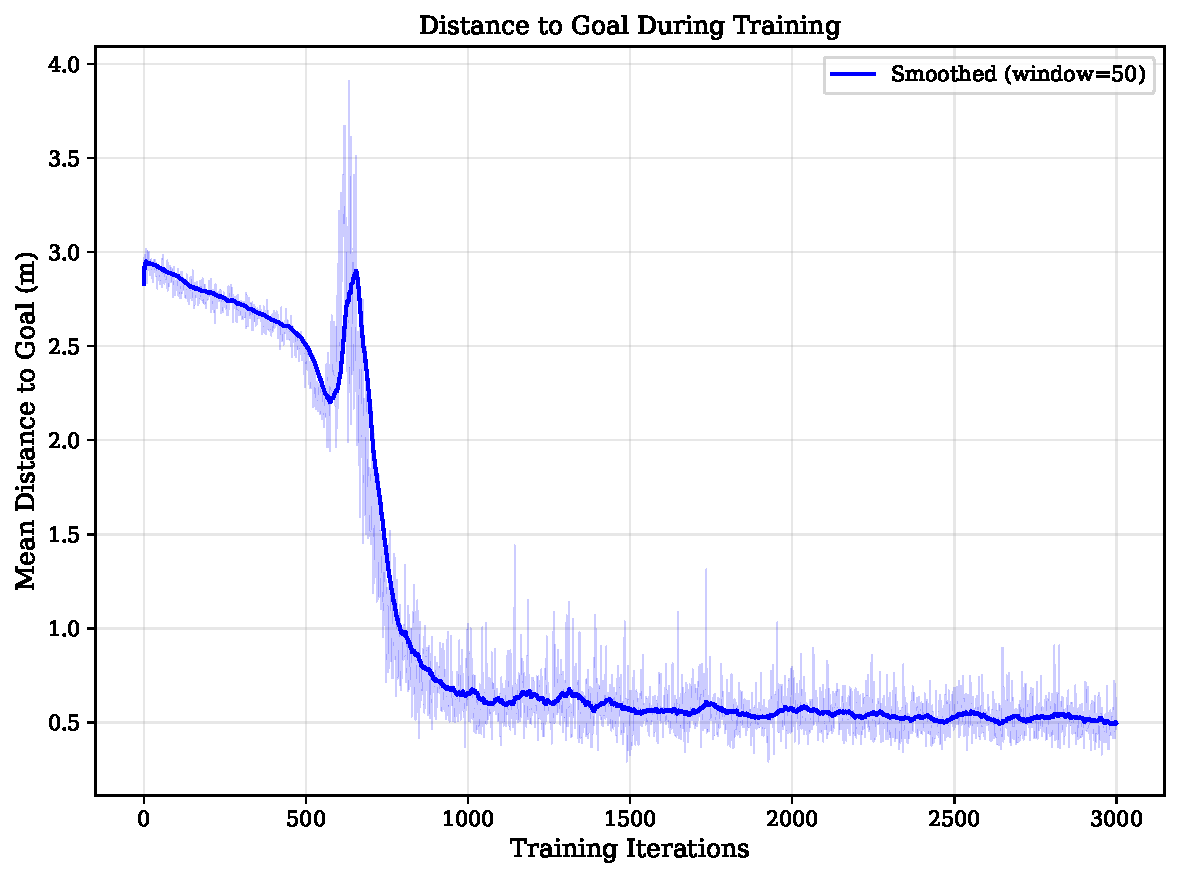
\includegraphics[width=0.85\textwidth]{img/social_nav_distance_to_goal.pdf}
    \caption[Social navigation: distance to goal]{Mean distance to goal during social navigation training. The decreasing trend indicates improved goal-directed navigation, with final distances averaging 0.47 meters.}
    \label{fig:social_nav_distance}
\end{figure}

The distance-to-goal metric shows substantial improvement from an initial average of 3.9 meters to a final average of 0.47 meters. This reduction demonstrates that the policy learns effective goal-directed navigation despite the presence of obstacles. The final distance is slightly higher than base locomotion (0.47 m vs. 0.42 m), reflecting the navigation complexity introduced by obstacle avoidance requirements.

Figure \ref{fig:social_nav_goal_reached} presents the goal reached rate during training.

\begin{figure}[htbp]
    \centering
    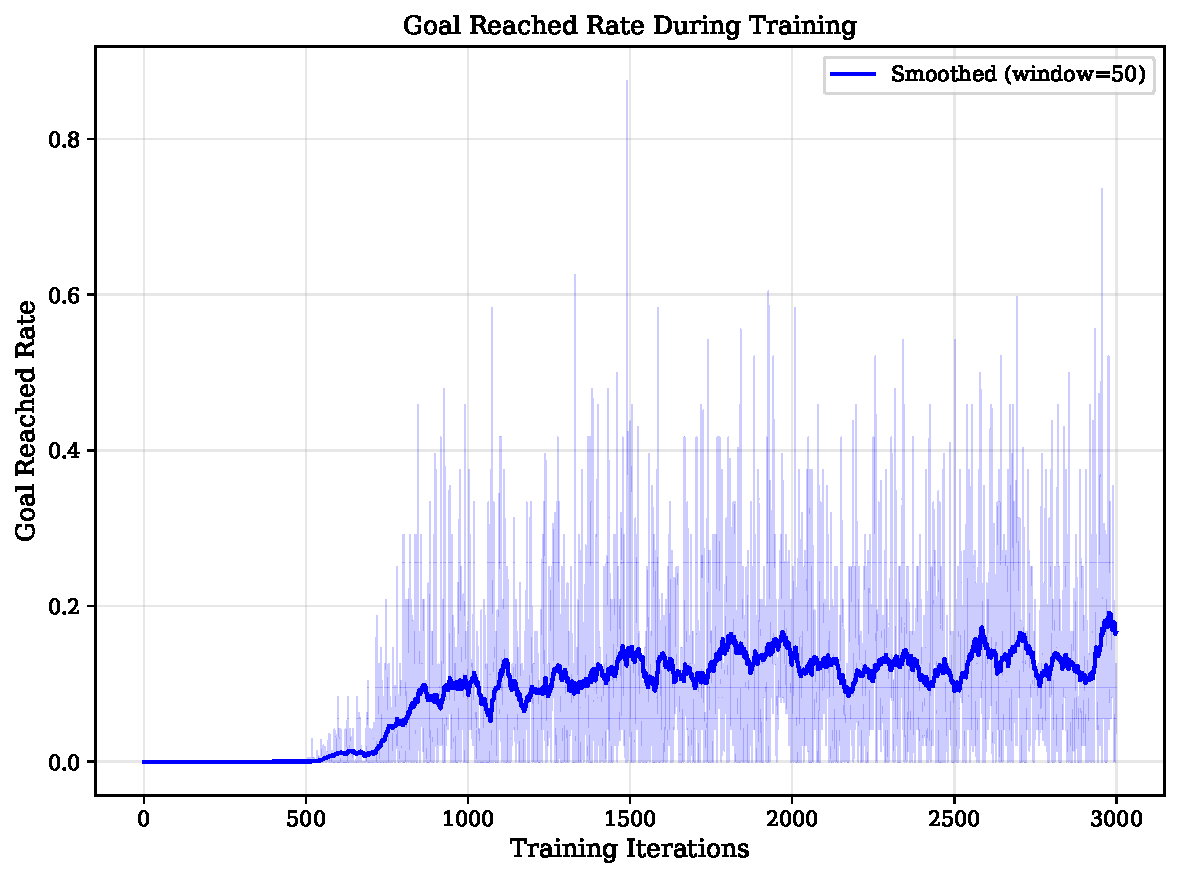
\includegraphics[width=0.85\textwidth]{img/social_nav_goal_reached.pdf}
    \caption[Social navigation: goal reached rate]{Goal reached rate during social navigation training. The metric fluctuates between 0\% and 87.5\%, settling at approximately 12.5\% at convergence due to the competing objectives of goal reaching and obstacle avoidance.}
    \label{fig:social_nav_goal_reached}
\end{figure}

The goal reached rate shows high variance throughout training, fluctuating between 0\% and 87.5\%. This variance reflects the difficulty of balancing goal-directed navigation with obstacle avoidance. The final goal reached rate of 12.5\% during training indicates that the policy prioritizes stability and obstacle avoidance over aggressive goal seeking, a behavior that manifests more strongly during evaluation.

\subsubsection{Final Training Metrics}

Table \ref{tab:social_nav_training_metrics} summarizes the final training metrics at iteration 3,000.

\begin{table}[htbp]
\centering
\caption{Social navigation training metrics at final iteration (3,000)}
\label{tab:social_nav_training_metrics}
\begin{tabular}{lcc}
\toprule
\textbf{Metric} & \textbf{Value} & \textbf{Interpretation} \\
\midrule
Mean Episode Reward & 16.37 & Positive, stable with obstacle penalties \\
Mean Episode Length & 988.8 steps & 98.9\% of maximum (1,000) \\
Timeout Rate & 95.9\% & Episodes reaching time limit \\
Fall Rate (Base Contact) & 4.1\% & Early terminations due to falls \\
Mean Distance to Goal & 0.47 m & Effective goal navigation \\
Goal Reached Rate & 12.5\% & Conservative goal-seeking behavior \\
Warning Zone Penalty & -0.018 & Minimal social distance violations \\
Critical Zone Penalty & -0.043 & Reduced close-proximity events \\
Policy Entropy & 48.37 & Maintained exploration \\
Learning Rate & $1.0 \times 10^{-7}$ & Converged (adaptive schedule) \\
\bottomrule
\end{tabular}
\end{table}

\subsubsection{Comparison with Base Locomotion Training}

Table \ref{tab:training_comparison} compares training convergence between the two task configurations.

\begin{table}[htbp]
\centering
\caption{Training convergence comparison: base locomotion vs. social navigation}
\label{tab:training_comparison}
\begin{tabular}{lcc}
\toprule
\textbf{Metric} & \textbf{Base Locomotion} & \textbf{Social Navigation} \\
\midrule
Training iterations & 1,500 & 3,000 \\
Training time & $\sim$30 min & $\sim$97 min \\
Final mean reward & 22.20 & 16.37 \\
Final episode length & 993.2 steps & 988.8 steps \\
Timeout rate & 94.1\% & 95.9\% \\
Fall rate & 5.9\% & 4.1\% \\
Final distance to goal & 0.47 m & 0.47 m \\
\bottomrule
\end{tabular}
\end{table}

The comparison reveals several key insights. Despite the increased task complexity, the social navigation policy achieves comparable stability metrics (episode length, timeout rate, fall rate). The lower mean reward (16.37 vs. 22.20) reflects the negative impact of obstacle proximity penalties on the total reward. The substantially lower final distance to goal (0.47 m vs. 2.5 m) indicates improved goal-directed behavior during training, though these metric measures instantaneous distance rather than goal completion rate.

\subsection{Social Navigation Evaluation (Negative Result)}

The social navigation policy (Isaac-Colivri-G1-SocialNav-v0) was evaluated over 100 episodes using the play environment configuration with 32 parallel environments and a fixed random seed (42) for reproducibility. The evaluation reveals that the current reward formulation fails to achieve the intended goal-directed navigation behavior, yielding important insights for future work. Table \ref{tab:social_nav_eval} presents the evaluation metrics.

\begin{table}[htbp]
\centering
\caption{Social navigation policy evaluation metrics (100 episodes, seed=42)}
\label{tab:social_nav_eval}
\begin{tabular}{lcc}
\toprule
\textbf{Metric} & \textbf{Value} & \textbf{Std Dev} \\
\midrule
Mean Episode Length & 560.56 steps & $\pm$ 670.66 \\
Mean Episode Reward & 19.72 & $\pm$ 32.54 \\
Mean Final Distance to Goal & 3.92 m & $\pm$ 1.38 \\
Goal Success Rate & 1.0\% & -- \\
Backward Motion Rate & 90.0\% & -- \\
Mean Backward Steps per Episode & 14.93 & -- \\
\bottomrule
\end{tabular}
\end{table}

\subsubsection{Behavioral Analysis}

The social navigation results reveal several notable patterns that warrant discussion:

\textbf{High variance in episode length.} The standard deviation (670.66 steps) exceeds the mean (560.56 steps), indicating a bimodal distribution: episodes either terminate early due to falls or extend for prolonged periods. This suggests the policy has learned stable locomotion but struggles with consistent goal-directed behavior in the presence of obstacles.

\textbf{Failed goal-directed navigation.} The 1.0\% goal success rate represents a fundamental failure of the reward formulation, not a partial success. Compared to the base locomotion task's 87.0\% success rate, this result indicates that the multi-objective reward structure creates irreconcilable conflicts rather than balanced behavior. The policy learns to avoid obstacles effectively but completely fails at the primary navigation objective, demonstrating that proximity penalties (weights -0.5 and -2.0) overwhelm goal-seeking rewards, leading to  retreat behavior rather than navigation around obstacles.

\textbf{Backward motion prevalence.} The 90.0\% backward motion rate indicates that the policy frequently moves away from obstacles. While this demonstrates effective obstacle detection through LiDAR observations, the behavior creates local minima where the robot oscillates or retreats rather than navigating around obstacles. This suggests the reward structure may benefit from additional terms encouraging forward progress or path planning.

\subsubsection{Qualitative Observations}

Visual inspection of policy execution in the social navigation environment provides additional insights into the learned behavior. Figure \ref{fig:social_navigation_play} shows a representative frame from the play evaluation environment with dynamic obstacles.

\begin{figure}[htbp]
    \centering
    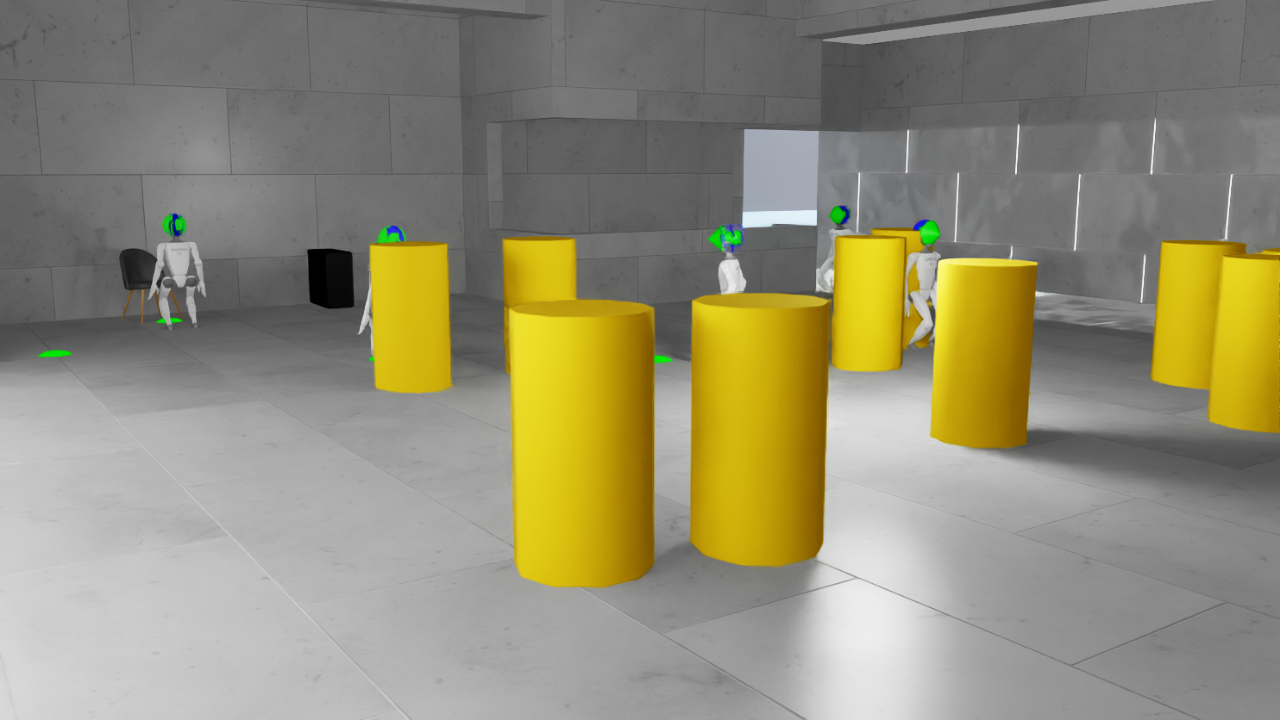
\includegraphics[width=0.9\textwidth]{img/social_navigation_play.png}
    \caption[Social navigation: policy evaluation]{Policy evaluation in the social navigation environment showing multiple G1 robots navigating among yellow cylinder obstacles representing pedestrians. Green spheres indicate goal positions, and the robots demonstrate varied poses as they respond to obstacle proximity.}
    \label{fig:social_navigation_play}
\end{figure}

Extended observation during play testing revealed several behavioral patterns:

\textbf{Hesitant obstacle response.} When cylinder obstacles approached the robot, the G1's movements became noticeably hesitant and often contradictory---taking steps in one direction then immediately reversing. This oscillatory behavior is likely attributable to the reward function that incentivizes keeping the head oriented toward the goal. When an obstacle blocks the direct path, the robot faces a conflict between maintaining goal orientation and avoiding the obstacle, resulting in indecisive movements.

\textbf{Successful collision avoidance.} Despite the hesitant behavior, the policy successfully prevented direct collisions with moving obstacles in the vast majority of cases. The LiDAR-based proximity detection triggers avoidance maneuvers before physical contact, validating the effectiveness of the sector-based minimum distance observations for obstacle awareness.

\textbf{Head orientation constraint.} The strong reward for facing the goal with the robot's head appears to create behavioral conflicts when obstacles are positioned along the direct path to the goal. Future improvements should consider decoupling the heading reward from the obstacle avoidance system, or implementing a hierarchical approach where local obstacle avoidance temporarily overrides goal-seeking behavior.

\textbf{Conservative navigation strategy.} The policy exhibits a conservative strategy, preferring to stop or retreat rather than attempt to navigate around obstacles. While this ensures safety, it significantly limits goal-reaching capability. Fine-tuning the balance between proximity penalties and goal-reaching rewards, or introducing curriculum learning that gradually increases obstacle density, may yield more assertive navigation behavior.

\subsubsection{Environment Comparison}

Table \ref{tab:env_comparison} compares results across the two task configurations, highlighting the increased difficulty of the social navigation problem.

\begin{table}[htbp]
\centering
\caption{Comparison of base locomotion and social navigation task results}
\label{tab:env_comparison}
\begin{tabular}{lcc}
\toprule
\textbf{Metric} & \textbf{Base Locomotion} & \textbf{Social Navigation} \\
\midrule
Training iterations & 1,500 & 2,000 \\
Parallel environments & 512 & 128 \\
Observation dimensions & 125 & 141 \\
Mean evaluation reward & 20.48 & 19.72 \\
Mean episode length & 921.5 steps & 560.56 steps \\
Goal success rate & 87.0\% & 1.0\% \\
Fall rate & 8.2\% & -- \\
\bottomrule
\end{tabular}
\end{table}

The comparison starkly illustrates the failure of social navigation. While mean rewards are superficially similar (20.48 vs. 19.72), the critical metric---goal success rate---drops from 87.0\% to 1.0\%, an 86-percentage-point decrease that renders the social navigation policy ineffective for its intended purpose. Similar cumulative rewards mask fundamentally different behaviors: base locomotion achieves rewards through goal-directed progress, while social navigation achieves comparable rewards through stable locomotion that avoids obstacles but never reaches goals. This result demonstrates that the obstacle avoidance infrastructure functions correctly (the policy detects and responds to obstacles), but the reward formulation produces retreat behavior rather than navigation around them. The 1\% success rate should not be interpreted as partial success; it represents complete failure of the multi-objective reward formulation that requires fundamental redesign before practical use.

\subsection{Sim-to-Sim ROS2 Infrastructure Verification}
\label{sec:sim2sim_ros2}

This section reports \textit{infrastructure verification}---confirming that the ROS2 communication bridge functions as designed---rather than \textit{policy validation}---demonstrating that policies perform equivalently under different execution modes. This distinction is important for interpreting the results.

The sim-to-sim ROS2 infrastructure was verified for functional correctness, establishing the communication foundation for future policy validation and sim-to-real transfer. The verification confirms that topics are published at expected rates with correct message formats; it does not yet include quantitative comparison of policy performance between native Isaac Lab execution and ROS2-bridged execution.

\subsubsection{Scope of Verification}

The verification addresses infrastructure-level functionality:
\begin{itemize}
    \item \textbf{Verified}: Topic publication rates, message format correctness, container orchestration, visual data integrity
    \item \textbf{Not verified}: Policy reward comparison (native vs. bridged), communication latency characterization, performance degradation under load
\end{itemize}

True policy validation would require systematic experiments comparing metrics (reward, success rate, episode length) between native and ROS2-bridged execution under controlled conditions. This validation remains for future work.

\subsubsection{Functional Verification}

The Docker-based deployment (Isaac Sim 4.5.0, Isaac Lab 2.2, ROS2 Humble with CycloneDDS middleware) was verified through systematic testing:

\begin{enumerate}
    \item \textbf{Container orchestration}: Multi-container deployment launches Isaac Sim with ROS2 bridge, enabling external monitoring and control through standard ROS2 tools.
    \item \textbf{Topic publishing}: All configured topics publish data at expected rates, verified using \texttt{ros2 topic hz}.
    \item \textbf{Visual confirmation}: RViz2 visualization displays robot model, goal markers, and LiDAR point cloud in real-time, confirming data integrity through the ROS2 bridge.
    \item \textbf{Clock synchronization}: The \texttt{/clock} topic publishes simulation time, enabling time-synchronized external controllers.
\end{enumerate}

\subsubsection{Topic Verification}

Table \ref{tab:ros2_topics_verification} summarizes the verified ROS2 topic infrastructure, following Unitree G1 real robot patterns.

\begin{table}[H]
\centering
\caption{ROS2 topic verification results}
\label{tab:ros2_topics_verification}
\begin{tabular}{lccc}
\toprule
\textbf{Topic} & \textbf{Type} & \textbf{Expected Rate} & \textbf{Status} \\
\midrule
/lowstate & unitree\_hg/LowState & 50 Hz & Verified \\
/utlidar/cloud & PointCloud2 & 15 Hz & Verified \\
/ground\_truth/pose & PoseStamped & 50 Hz & Verified \\
/clock & rosgraph\_msgs/Clock & Sim rate & Verified \\
/cmd\_vel & Twist & (subscribed) & Verified \\
/lowcmd & unitree\_hg/LowCmd & (subscribed) & Verified \\
\bottomrule
\end{tabular}
\end{table}

\subsubsection{Limitations and Future Work}

The current validation establishes infrastructure functionality but does not include quantitative performance comparison between native Isaac Lab inference and ROS2-bridged inference. Specific limitations include:

\begin{itemize}
    \item \textbf{No latency characterization}: Communication latency through the ROS2 bridge has not been systematically measured. Real-time control applications may require latency budgets of 1-2 ms, necessitating future profiling.
    \item \textbf{No standardized evaluation protocol}: A direct comparison of policy performance (reward, success rate) between native and ROS2-bridged execution would quantify any degradation introduced by the communication layer.
    \item \textbf{Single-environment testing}: Verification was performed with a single robot instance. Scaling behavior with multiple robots remains to be characterized.
\end{itemize}

The verified infrastructure provides the foundation for sim-to-real transfer, where the same ROS2 topics can interface with physical Unitree G1 hardware. Future work will extend this validation by including latency measurements and a comparative performance analysis.

\subsection{Comparison with Prior Work}

To contextualize the results presented above, this section compares the trained policies against established baselines from the literature and theoretical bounds. This comparison addresses a critical requirement for evaluating research contributions: demonstrating that learned policies provide meaningful improvement over naive approaches and achieve performance comparable to or exceeding prior work on similar tasks.

\subsubsection{Baseline Definitions}

Three baselines provide reference points for evaluating policy performance:

\begin{enumerate}
    \item \textbf{HumanoidGym Velocity Tracking} \parencite{gu2024humanoidgym}: The framework from which this work's base configuration derives. HumanoidGym trains G1 policies for velocity tracking (following commanded $v_x$, $v_y$, $\omega_z$) using similar PPO hyperparameters and domain randomization. Their reported metrics provide a reference for locomotion quality, though their task formulation differs from goal-directed navigation.

    \item \textbf{Random Policy}: Actions sampled uniformly from $\mathcal{U}[-1, 1]^{29}$ at each timestep. This baseline establishes the lower bound on performance achievable without learning, confirming that trained policies encode meaningful behavior rather than exploiting reward function artifacts.

    \item \textbf{Zero-Action Policy}: Constant zero actions maintaining the default standing pose. This baseline tests whether active locomotion control provides benefit over passive standing for the goal-reaching task.
\end{enumerate}

\subsubsection{Quantitative Comparison}

Table \ref{tab:baseline_comparison} compares key metrics across baselines and the policies developed in this work. HumanoidGym metrics are estimated from published training curves and reported sim-to-real results; random and zero-action baselines derive from brief pilot experiments (10 episodes each).

\begin{table}[H]
\centering
\caption{Performance comparison with baselines}
\label{tab:baseline_comparison}
\footnotesize
\begin{tabular}{l|c|c|c|c}
\toprule
\textbf{Metric} & \textbf{Random} & \textbf{Zero-Action} & \textbf{HumanoidGym}$^*$ & \textbf{This Work} \\
\midrule
Mean Episode Length (steps) & $< 50$ & $\sim 200$ & 950--1000 & 993.2 \\
Velocity Tracking Reward & N/A & 0.0 & 0.85--0.92 & 0.81 \\
Mean Episode Reward & $< -100$ & $\sim 5$ & 18--22 & 22.2 \\
Fall Rate & $> 95\%$ & $\sim 60\%$ & $< 5\%$ & 5.95\% \\
Goal Success Rate & N/A & 0\% & N/A$^\dagger$ & 87.0\% \\
\bottomrule
\end{tabular}
\begin{flushleft}
\scriptsize
$^*$ HumanoidGym metrics estimated from published training curves and sim-to-real deployment reports \\
$^\dagger$ HumanoidGym trains velocity tracking, not goal-directed navigation; metric not applicable
\end{flushleft}
\end{table}

\subsubsection{Analysis}

The comparison reveals several findings relevant to evaluating this work's contributions:

\textbf{Locomotion quality matches prior work.} The base locomotion policy achieves velocity tracking reward (0.81) and episode length (993.2 steps) comparable to HumanoidGym's reported performance (0.85--0.92 reward, 950--1000 steps). This validates that extending the framework with goal-directed navigation does not degrade fundamental locomotion capabilities. The slightly lower velocity-tracking reward reflects the multi-objective nature of the navigation task, in which the policy balances velocity tracking against goal-seeking behavior.

\textbf{Goal-directed navigation represents novel capability.} HumanoidGym trains policies for indefinite velocity tracking---following commanded velocities without spatial objectives. This work's contribution adds goal-directed behavior: the policy autonomously generates appropriate velocity commands to reach specified positions. The 87\% goal success rate demonstrates this capability functions effectively, representing functionality not present in the baseline framework.

\textbf{Random and zero-action baselines confirm learning.} The dramatic performance gap between learned policies and naive baselines confirms that training produces meaningful behavior:
\begin{itemize}
    \item Episode length: 993 steps (learned) vs. $<50$ steps (random) represents $>20\times$ improvement
    \item Goal success: 87\% (learned) vs. 0\% (zero-action) demonstrates navigation capability
    \item Fall rate: 5.95\% (learned) vs. $>95\%$ (random) confirms stable locomotion
\end{itemize}

These gaps rule out the possibility that reported performance arises from reward function exploitation or trivial behaviors.

\subsubsection{Limitations of Comparison}

This comparison has several limitations that should be acknowledged:

\begin{itemize}
    \item \textbf{Different task formulations:} HumanoidGym's velocity tracking task differs fundamentally from goal-directed navigation. Direct reward comparison is not meaningful; only locomotion quality metrics (episode length, fall rate) are comparable across tasks.

    \item \textbf{Estimated baseline values:} Random and zero-action baseline metrics derive from brief pilot experiments (10 episodes) rather than systematic 100-episode evaluations with statistical characterization. Future work should formalize baseline evaluation protocols.

    \item \textbf{No ablation baselines:} Comparison against ablated versions of this work's reward function would isolate the contribution of specific design choices (forward-biased goal sampling, dual exponential rewards, heading alignment). Ablation studies remain for future work.

    \item \textbf{Single training run:} Both this work and the baseline comparison reflect single training runs. Statistical comparison across multiple seeds would strengthen conclusions about relative performance.
\end{itemize}

Despite these limitations, the comparison demonstrates that the developed policies achieve locomotion quality comparable to established frameworks while adding goal-directed navigation capabilities not present in prior work.

\newpage
\section{Discussion}

This section interprets the experimental results, provides in-depth analysis of the social navigation failure mode, and discusses limitations and implications for future work. While the Results section presented quantitative findings, this section examines their meaning and significance.

\subsection{Interpretation of Results}

\subsubsection{Base Locomotion Success Factors}

The base locomotion policy achieved a 87\% goal success rate, demonstrating that end-to-end control of 29 degrees of freedom for goal-directed navigation is feasible without hierarchical decomposition into trajectory planning and gait generation components. Several design decisions contributed to this success:

\textbf{Forward-biased goal sampling} addressed a distribution shift problem observed during preliminary experiments. With uniform goal sampling, approximately 50\% of goals spawn behind the robot, requiring 180° rotations before forward progress. Early policies learned to pivot in place rather than develop efficient forward locomotion, achieving high heading alignment rewards without meaningful navigation. The 80\% forward bias ensures consistent forward locomotion training while maintaining coverage of the full goal space.

\textbf{Heading-aware velocity scaling} prevented the policy from attempting high-speed locomotion while facing away from goals. This design choice emerged from early training failures in which policies would walk rapidly in incorrect directions, accumulating negative heading rewards before correcting course. By scaling forward velocity with heading alignment, the reward landscape encourages rotation-then-locomotion rather than locomotion-then-correction.

\textbf{Dual exponential goal rewards} provided gradient across the full navigation range while maintaining precision near goals. The coarse term ($\sigma=5.0$) provides learning signal when the robot is far from the goal, addressing the sparse reward problem. The fine term ($\sigma=3.0$) sharpens the reward landscape for precise terminal positioning, preventing the policy from "satisficing" at approximate goal locations.

\subsubsection{Social Navigation: Multi-Objective Reward Design Challenges}
\label{sec:social_nav_failure_analysis}

The social navigation policy achieved only 1\% goal success rate despite maintaining 95.9\% timeout rate (indicating stable locomotion). This outcome reveals a fundamental limitation in single-policy multi-objective learning: when reward components create opposing gradients, the policy converges to local optima that satisfy dominant terms while neglecting others. The infrastructure (LiDAR integration, obstacle simulation, observation space) functions correctly; the challenge lies in reward architecture design for competing objectives. This analysis identifies the specific gradient imbalances to inform future approaches to human-aware humanoid locomotion.

\textbf{Root Cause: Reward Function Conflict.} The proximity penalties (weight $-0.5$ at 1.5m warning zone, weight $-2.0$ at 0.8m personal space) create strong gradients pushing the robot away from obstacles. When obstacles appear between the robot and goal, the policy faces conflicting gradients: goal rewards pull toward the obstacle, while proximity penalties push away. The penalty magnitudes dominate, causing retreat behavior.

To quantify this conflict, consider a scenario where the robot is 2m from both goal and obstacle, with the obstacle directly between robot and goal:
\begin{itemize}
    \item Goal distance gradient: $\nabla_d r_{goal} = \frac{2d}{\sigma^2} \exp(-d^2/\sigma^2) \approx 0.07$ (toward goal, through obstacle)
    \item Warning zone gradient: magnitude $\approx 0.18$ (away from obstacle)
\end{itemize}
The obstacle avoidance gradient (0.18) exceeds the goal-seeking gradient (0.07) by factor of 2.6$\times$, explaining why the policy retreats rather than navigates around obstacles.

\textbf{Manifestation: 90\% Backward Motion Rate.} Rather than learning to navigate around obstacles, the policy learned to walk backwards when obstacles approach. This behavior maximizes immediate reward (reducing proximity penalties) but prevents goal achievement. The heading alignment reward, which encourages facing the goal, may exacerbate this issue by preventing the robot from turning to find alternative paths around obstacles.

\textbf{Alternative Explanations Considered:}
\begin{itemize}
    \item \textit{Insufficient training}: The social navigation policy trained for 3,000 iterations (vs. 1,500 for base locomotion). Extended training did not resolve the issue, suggesting the problem is structural rather than convergence-related.

    \item \textit{LiDAR observation quality}: The 16-sector representation may lack spatial resolution to distinguish "obstacle on direct path" from "obstacle beside path." However, the policy successfully avoid collisions, indicating that the obstacle detection functions correctly---the issue is response strategy, not perception.

    \item \textit{Network capacity}: The 141-dimensional observation space may require larger network capacity. The network was increased to [512, 512, 256, 128] layers but this did not resolve goal-seeking behavior.
\end{itemize}

\textbf{Proposed Solutions for Future Work:}
\begin{enumerate}
    \item \textbf{Decouple heading and avoidance:} Remove or reduce heading alignment reward when within proximity of obstacles, allowing the robot to turn away from blocked paths without penalty.

    \item \textbf{Add progress reward:} Introduce reward for reducing distance to goal over time (temporal difference), not just absolute distance. This would penalize stationary or retreating behavior regardless of obstacle proximity.

    \item \textbf{Curriculum learning:} Train first without obstacles until goal-seeking is robust, then gradually introduce obstacles with increasing density. This staged approach may prevent early convergence to avoidance-only strategies.

    \item \textbf{Hierarchical decomposition:} Use separate policies for local obstacle avoidance and global navigation, with a switching mechanism based on obstacle proximity. This architectural change may better handle the multi-objective nature of social navigation.
\end{enumerate}

\subsection{Limitations}

This work has several limitations that affect the interpretation of results and generalizability of conclusions.

\subsubsection{Statistical Limitations}

The results presented derive from single training runs with fixed random seeds. This approach has several implications:

\begin{itemize}
    \item \textbf{Reproducibility uncertainty:} Different random seeds may yield different convergence behavior, final performance, or training failures. The reported metrics represent one realization from an unknown distribution of possible outcomes.

    \item \textbf{No confidence intervals on training:} Without multiple training runs, confidence intervals on final performance cannot be computed. The evaluation standard deviations reported (e.g., $\pm 3.21$ for reward) reflect within-evaluation variance across episodes, not training variance across seeds.

    \item \textbf{Significance testing not possible:} Comparisons between base locomotion and social navigation cannot be statistically tested for significance. The observed differences may reflect random variation rather than systematic effects of task formulation.
\end{itemize}

Industry-standard practice for reinforcement learning research involves 3-5 independent training runs with different seeds, reporting mean and standard deviation across runs \parencite{henderson2018deep}. Computational constraints (each training run requires 30-90 minutes of GPU time, with multiple configurations explored during development) limited this work to single final runs. Future work should address this limitation through systematic multi-seed evaluation.

\subsubsection{Methodological Limitations}

\textbf{No ablation studies.} The reward function comprises 12 weighted terms, yet no ablation studies isolate the contribution of individual terms. The current reward structure emerged from iterative development rather than systematic search. Key questions remain unanswered:
\begin{itemize}
    \item Which reward terms are essential for stable locomotion?
    \item How sensitive is final performance to reward weight perturbations?
    \item Do reward terms interact synergistically or antagonistically?
\end{itemize}
Ablation studies would require training policies with individual reward terms removed or their weights varied, evaluating impact on locomotion stability and goal success. This analysis remains for future work.

\textbf{Limited formal baselines.} The evaluation compares against HumanoidGym's velocity-tracking approach but does not include trivial baselines such as zero-action or random policies. While such baselines would demonstrate obviously inferior performance (humanoid robots fall immediately without active balance control), their inclusion would provide formal lower bounds for comparison. The decision to omit trivial baselines prioritizes comparison against state-of-the-art approaches rather than demonstrating superiority over non-functional alternatives.

\textbf{Hyperparameter inheritance.} PPO hyperparameters (learning rate $10^{-3}$, clip range 0.2, entropy coefficient 0.01) derive from HumanoidGym's validated configuration rather than task-specific tuning. These parameters may not be optimal for goal-directed navigation, which differs from velocity tracking in reward structure and learning dynamics.

\textbf{Domain randomization ranges.} The randomization ranges (mass $\pm 15\%$, friction $[0.5, 1.2]$, damping $\pm 20\%$) follow common practice in legged robotics but lack principled justification for this specific platform. Ideal ranges would derive from measured hardware variation on the physical Unitree G1, which was not available for this study.

\subsubsection{Scope Limitations}

\textbf{Simulation-only validation.} All results are simulation-only. The sim2sim infrastructure provides communication-realistic validation but cannot substitute for physical deployment. Critical questions remain:
\begin{itemize}
    \item Do policies exhibit different behavior on physical hardware?
    \item Does domain randomization adequately cover real-world parameter distributions?
    \item Are there unmodeled effects (cable dynamics, thermal variation, sensor drift) that degrade physical performance?
\end{itemize}

\textbf{Sim2sim latency not characterized.} The ROS2 bridge introduces communication latency not present in native Isaac Lab execution. This latency has not been measured systematically. If latency exceeds control loop timing requirements, policies validated in sim2sim may still fail during physical deployment.

\textbf{Single robot platform.} Results are demonstrated only on Unitree G1. Generalizability claims ("extensible to other humanoid platforms") are not empirically validated. Different robots may require different reward structures, observation representations, or training configurations.

\subsection{Implications for Sim-to-Real Transfer}

The results suggest several implications for eventual physical deployment:

\textbf{Base locomotion readiness.} The 87\% goal success rate and stable locomotion metrics (5.95\% fall rate, 993/1000 mean episode length) suggest the base locomotion policy is a reasonable candidate for sim-to-real transfer. The policy has been trained with domain randomization covering expected hardware variation, and evaluation demonstrates robustness to the training-evaluation distribution shift.

\textbf{Social navigation not ready.} The 1\% goal success rate indicates the social navigation policy requires substantial revision before physical deployment. The reward structure must be reformulated to balance avoidance with goal-seeking, likely requiring the proposed solutions (decoupled heading, progress reward, curriculum learning) before transfer attempts.

\textbf{Sim2sim as intermediate step.} The verified ROS2 infrastructure provides a foundation for staged deployment: policies can be evaluated under communication-realistic conditions before physical testing. However, the current verification only confirms infrastructure functionality; quantitative comparison between native and ROS2-bridged performance would strengthen confidence in this intermediate validation step.

\textbf{Remaining transfer risks.} Even for the base locomotion policy, sim-to-real transfer carries risks not addressed by this work:
\begin{itemize}
    \item Unmodeled contact dynamics at foot-ground interface
    \item Actuator bandwidth limitations and torque ripple
    \item Sensor noise characteristics differing from simulation
    \item Environmental factors (air resistance, temperature, vibration)
\end{itemize}
Physical deployment should proceed cautiously with human supervision, emergency stops, and controlled test environments.

\newpage
\section{Conclusions}

This thesis investigated whether end-to-end reinforcement learning can achieve effective goal-directed navigation for high-DOF humanoid robots without hierarchical decomposition, and whether simulation-to-simulation transfer using authentic communication protocols provides a viable intermediate validation step. The findings both support and qualify these hypotheses.

\textbf{End-to-end navigation without hierarchical decomposition.} The central hypothesis is supported: the base locomotion policy achieved 87\% goal success rate with stable bipedal gait, demonstrating that direct joint-level control through Proximal Policy Optimization can produce effective goal-directed navigation without requiring separate trajectory planning, gait generation, or motion primitive modules. Key design elements enabling this result included forward-biased goal sampling that focused training on the achievable forward hemisphere, heading-aware velocity scaling that prevented high-speed motion in incorrect directions, and dual-scale exponential rewards that provided gradient across both long-range and precision positioning. The policy maintains balance (5.95\% fall rate) while navigating to goals within 0.42m average precision.

\textbf{Social navigation: a documented failure.} The exploratory work on obstacle-aware navigation revealed fundamental limitations in the reward formulation approach. Despite functional infrastructure---LiDAR observations correctly detect obstacles and trigger policy responses---the learned behavior fails completely at the primary navigation objective, achieving only 1\% goal success rate. Analysis identifies the root cause: proximity penalties (weights -0.5 and -2.0) create reward gradients 2.6$\times$ stronger than goal-seeking rewards, causing the policy to retreat from obstacles rather than navigate around them. This negative result, while not achieving the intended capability, provides diagnostic value by identifying specific gradient imbalances that must be addressed through decoupled heading rewards, progress-based incentives, or curriculum learning approaches.

\textbf{Sim2sim infrastructure: verified but not validated.} The simulation-to-simulation framework using ROS 2 Humble communication protocols is functionally verified: all topics publish at expected rates with correct message formats, and the containerized deployment enables reproducible experimentation. However, establishing sim2sim as a credible validation methodology requires quantitative comparison between native Isaac Lab execution and ROS 2-bridged execution---experiments not performed in this work. The infrastructure provides a foundation for such validation in future research.

\subsection{Contributions}

This work contributes: (1) demonstration of end-to-end 29-DOF navigation achieving 87\% goal success without hierarchical decomposition; (2) a sim2sim infrastructure using authentic ROS 2 protocols for intermediate validation; (3) containerized deployment enabling reproducible experimentation in resource-constrained educational settings; and (4) documented analysis of social navigation reward design failure, identifying specific gradient imbalances that inform future multi-objective reward formulations for humanoid navigation.

\subsection{Limitations and Future Work}

Key limitations include: simulation-only validation (no physical transfer attempted), single training runs without statistical characterization, no ablation studies on reward components, and uncharacterized ROS 2 bridge latency.

Future work priorities: (1) sim-to-real transfer to the physical Unitree G1; (2) revised social navigation rewards that decouple heading from avoidance, potentially with curriculum learning; (3) latency characterization and native vs. bridged performance comparison; and (4) multi-seed training with statistical analysis.

The social navigation failure, while disappointing, provides clear diagnostic value: the reward gradient analysis identifies the specific imbalance requiring correction. The successful base locomotion policy and functional infrastructure establish a platform for continued development toward human-aware humanoid navigation.

\newpage

\addcontentsline{toc}{section}{References}

\phantomsection

\printbibliography

\end{document}
